\documentclass[12pt,a4paper]{article}

\renewcommand{\baselinestretch}{1.3}

\usepackage{cancel}
\usepackage{mathrsfs}
\usepackage{natbib}
\usepackage{rotating}
\usepackage{multicol}
\usepackage{verbatim}
\usepackage{eufrak}
\usepackage[left=1.5cm,right=1.5cm,top=2cm,bottom=2.5cm]{geometry}
\usepackage{setspace}
\usepackage{indentfirst}
\usepackage[T2A]{fontenc}
\usepackage[russian]{babel}
\usepackage[utf8]{inputenc}
\usepackage{amsmath}
\usepackage{multicol}
\usepackage{verbatim}
\usepackage{eufrak}
\usepackage{subfiles}
\usepackage{amsxtra}
\usepackage{amssymb}
\usepackage{graphicx}
\usepackage{tikz}
\usepackage{comment}
\usepackage{enumerate}
\usepackage{wrapfig}
\usepackage{verbatim}
\usepackage{amsmath}
\usetikzlibrary{calc}
\pagestyle{plain}

\usepackage{mathtools}
\DeclarePairedDelimiter{\ceil}{\lceil}{\rceil}

\RequirePackage{caption}
\DeclareCaptionLabelSeparator{dot}{ . }
\captionsetup{justification=centering, labelsep=dot}

\begin{document}

{\large \hspace{4.5 cm} Введение в топологию $\bullet$ Общая топология}

\vspace{-1.5ex}

\hrulefill

\fontsize{14.4pt}{5.5mm}\selectfont

\vspace{-3ex}

\hrulefill

\tableofcontents
\newpage 

\section{Про топологию}

Топология \textbf{изучает} свойства пространств, сохраняющихся при непрерывных преобразованиях. Делится на общую (завершенный раздел, переживший период бурного развития) и современную. 

\textbf{Общая топология} --- элементарная, т.е. не требует предварительных глубоких познаний, и является фундаментом математики. Основные объекты изучения --- топологические пространства и непрерывные отображения. 

\textbf{Современная топология} состоит из многих разделов, среди которых \textbf{алгебраическая} --- изучает топологические пространства алгебраическими методами, т.е. проецирует топологию на алгебру, рассматривает топологические пространства, имеющие хорошие комбинаторные свойства, --- дифференциальная, объектами которой являются пространства, снабженные дополнительной дифференциальной структурой, и методы дифференциального исчисления, геометрическая, связанная с пространствами малой размерности, и другие. Стоит отметить, что разделы не изолированы, а взаимодействуют друг с другом. 

\section{Метрические пространства}

\subsection{Метрика}

\textbf{Определение.} Метрика на множестве X --- функция $\rho\!\!: X \times X \to [0; +\infty]$, удовлетворяющая следующим условиям:

$(1) \; \rho(x, y) = \rho(y, x) \quad \forall x, y \in X;$

$(2) \; \rho(x, x) = 0 \quad \forall x \in X;$

$(3) \; \rho(x, z) \leq \rho(x, y) + \rho(y, z) \quad \forall x, y, z \in X$ --- неравенство треугольника; 

$(4) \; \rho(x, y) > 0 \quad \forall x \neq y$. 

Таким образом, мы аксиоматически задали способ определить расстояние, т.е. то, что понимать под расстоянием в общем случае. 

\textbf{Метрическое пространство} (x, $\rho)$ --- множество (точнее --- пара), снабженное метрикой. Если выполняется только (1)--(3), то $\rho$ называется полуметрикой, а $(x, \rho)$ --- полуметрическим пространством. 

\textbf{Пример 0}. Дискретная метрика

\begin{equation*}
\rho(x, y) = 
\begin{cases}
1, &\text{если $x \neq y$},\\
0, &\text{если $x = y$}.
\end{cases}
\end{equation*}

\textbf{Пример 1.} Классический

$x = \mathbb{R}, \; \rho(x, y) = |x - y|$. Легко проверить, что выполняются все аксиомы метрики, причем неравенство треугольника --- свойство модуля. 

\textbf{Пример 2.} Три метрики на $R^n$

$\bullet \; \rho_1(x, y) = \overset{n}{\underset{i = 1}{\sum}}|x_{i} - y_{i}|$, где $x = (x_1, ..., x_n) \in \mathbb{R}^n, y \in \mathbb{R}^n$. Для каждой координаты выполняется неравенство треугольника: просуммируем координаты и получим, что для суммы тоже выполняется. 

$\bullet \; \rho_2(x, y) = \sqrt{\overset{n}{\underset{i = 1}{\sum}}(x_{i} - y_{i})^2}$ --- <<обычное>> расстояние --- евклидова метрика. 

$\bullet \; \rho_{\infty}(x, y) = \underset{1 \leq i \leq n}{\max} |x_{i} - y_{i}|$ (пояснение: если вместо 1 или 2 стоит p, метрика выглядит так: $\rho_{p} = \sqrt[p]{\overset{n}{\underset{i = 1}{\sum}}(x_{i} - y_{i})^{p}}$, это --- пример для $p \to \infty$). 

\textbf{Пример 3.} X = C[a, b] --- множество всех непрерывных функций $[a, b] \to \mathbb{R}$. 

Равномерная метрика (также супметрика): $\rho(f, g) = \underset{t \in [a, b]}{\sup}|f(t) - g(t)|$. Т.к. функция непрерывна и ограничена, можно назвать max, а не sup. 

\textbf{Наблюдение.} В примерах 1-3 X --- векторное пространство над $\mathbb{R}\!\!: \rho(x, y) = \rho(x - y, 0)$ --- т.к. это пространства специального вида --- нормированные. 

\subsection{Норма}

\textbf{Определение.} Пусть X --- векторное пространство над $\mathbb{K}$ (где $\mathbb{K} = \mathbb{R}$ или $\mathbb{K} = \mathbb{C}).$ Функция $X \to [0; +\infty], \; x \in X \mapsto ||x||,$ называется \textbf{нормой} на X (т.е. мы аксиоматически определяем, что такое длина вектора, --- тогда говорят норма), если она удовлетворяет следующим условиям: 

(1) $||\lambda \cdot x|| = |\lambda| \cdot ||x||, \; \lambda \in \mathbb{K}, \; x \in X$ (т.е. $\lambda$ --- число, x --- вектор);

(2) аналог неравенства треугольника: $||x + y|| \leq ||x|| + ||y||, \; (x, y \in X)$ --- прим.: на плоскости сводится к неравенству треугольника; 

(3) $||x|| > 0 \quad \forall x \neq 0$ ($x = 0:$ из аксиомы (1) $\Rightarrow$ $||x|| = 0$). 

Пространство на X, снабженное нормой, --- \textbf{нормированное пространство.} Например, $(x, ||\cdot||).$

Если (1), (2) выполняются, а (3) --- нет, то это \textbf{полунорма}, соответственно пространство --- полунормированное. 

\textbf{Наблюдение.} Пусть $(x, ||\cdot||)$ --- нормированное пространство. Тогда $\rho(x, y) = ||x - y|| \; (x, y \in X)$ --- метрика на X, порожденная нормой.  

\textbf{Упражнение.} Проверить выполнение аксиом метрики для $\rho(x, y).$ 

$\bullet$ Всякая \textbf{норма порождает метрику}; 

$\bullet$ Подмножество метрического пространства --- метрическое пространство; 

$\bullet$ Подмножество нормированного пространства --- нормированное пространство;  

$\bullet$ Всякое метрическое пространство изометрично нормированному пространству (изометрия --- биекция между метрическими пространствами, сохраняющая расстояния между точками, --- \textit{мое} примечание.)

\textbf{Пример 4}. Три нормы на $\mathbb{K}^{n}$, порожденные метриками из Примера 2

$\bullet \; ||x||_{1} = \overset{n}{\underset{i = 1}{\sum}} |x_i|;$

$\bullet \; ||x||_{2} = \sqrt{\overset{n}{\underset{i = 1}{\sum}} |x_{i}|^2}$ --- евклидова норма; 

$\bullet \; ||x||_{\infty} = \underset{1 \leq i \leq n}{\max}|x_{i}|$. 

\textbf{Пример 5.} Равномерная норма на пространстве непрерывных функций $C[a, b],$ порожденная метрикой из Примера 3.

$||f|| = \underset{t \in [a, b]}{\sup}|f(t)|.$

\textbf{Обозначение.} Напомним, что если X, Y --- множества, то $Y^{X}$ --- множество всех отображений $X \to Y$. В частности, $\mathbb{K^N}$ --- множество числовых последовательностей в $\mathbb{K}$. 

\textbf{Пример 6.} $l^{\infty}(S)$ --- множество всех ограниченных функций на множестве S: $\{f \in \mathbb{K}^S:$ f ограничена\}. 

||f|| = $\underset{s \in S}{\sup} \; |f(s)|$ --- равномерная норма. Повторное замечание: непрерывная функция ограничена (сверху и снизу) --- достигает максимум, можно писать не sup, а max. 

Частный случай: пространство ограниченных последовательностей $l^{\infty} = l^{\infty}(\mathbb{N}).$ 

\textbf{Пример 7.} $l^{1} = \{x = (x_{i}) \in \mathbb{K^N}\!\!:$ ряд сходится\}, где $x_{i}$ --- числовая последовательность. 

Норма на $l^{1}$: $||x||_{1} = \underset{i = 1}{\overset{\infty}{\sum}}|x_{i}|.$ 

\textbf{Пример 8 (важный)}

$l^{2}$ (можно также писать $l_{2}$) = $\{x = (x_{i}) \in \mathbb{K}:$ ряд $\underset{i = 1}{\overset{\infty}{\sum}}|x_{i}|^2$ сходится\}. 

$l^{2}$ --- векторное подпространство в $\mathbb{K^N}$ --- следует из неравенства $(a + b)^2 \leq 2(a^2 + b^2), \; a, b \geq 0.$

\textbf{\textit{Мое} доказательство.} $l^{2}$ --- \textbf{векторное подпространство} в $\mathbb{K^N}$ --- 1) если $\underset{i = 1}{\overset{\infty}{\sum}}|x_{i}|^2 < \infty$, то и $\underset{i = 1}{\overset{\infty}{\sum}}|c \cdot x_{i}|^2 = \underset{i = 1}{\overset{\infty}{\sum}}|c||x_{i}|^2 = |c|\underset{i = 1}{\overset{\infty}{\sum}}|x_{i}|^2 < \infty$ для любого $c$ из $\mathbb{K},$ 2) $(a + b)^2 \leq 2(a^2 + b^2), \quad \forall a, b \geq 0,$ то есть ряд, составленный из $|x_{n} + y_{n}|^{2},$ сходится, т.к. каждый его элемент не больше суммы двух соответственных элементов $|x_{n}|^{2}, \; |y_{n}|^{2}$ сходящихся рядов. $\quad \square$ 

Норма на $l^2: ||x||_{2} = \sqrt{\underset{i = 1}{\overset{\infty}{\sum}}|x_{i}|^2}.$ 

\textbf{\textit{Мое} доказательство.} Проверим, что выполняются аксиомы нормы: 

(1) $||\lambda \cdot x|| = |\lambda| \cdot ||x||, \; \lambda \in \mathbb{K}, \; x \in X:\! \;  \sqrt{\underset{i = 1}{\overset{\infty}{\sum}}|\lambda \cdot x_{i}|^2} = \sqrt{\underset{i = 1}{\overset{\infty}{\sum}}\lambda^{2}|x_{i}|^2} = |\lambda|  \sqrt{\underset{i = 1}{\overset{\infty}{\sum}}|x_{i}|^2};$ 

(2) $||x + y|| \leq ||x|| + ||y||, \; (x, y \in X),$ то есть $||\sqrt{\underset{i = 1}{\overset{\infty}{\sum}}|(x + y)_{i}|^2} \leq \sqrt{\underset{i = 1}{\overset{\infty}{\sum}}|x_{i}|^2} + \sqrt{\underset{i = 1}{\overset{\infty}{\sum}}|y_{i}|^2}.$ Также следует из $(a + b)^{2} < a^{2} + b^{2}.$

(3) $||x|| > 0 \quad \forall x \neq 0$ (x = 0: из аксиомы (1) $\Rightarrow$ ||x|| = 0). $|x_{i}| \geq 0,$ причем равенство достигается, только когда $x_{i} = 0.$ Значит, $||x||_{2} = 0 \Leftrightarrow \forall x_{i} = 0,$ во всех остальных случаях $\exists |x_{i}| > 0 \Rightarrow ||x||_{2} > 0. \quad \square$

В некоторых пространствах норма исходит из скалярного произведения, поэтому  \textbf{напоминание из геометрии:}

\textbf{Определение.} Евклидово пространство --- аксиоматически определено скалярное произведение, а не расстояние. 

\textbf{Скалярное произведение} на E, где E --- векторное пространство над $\mathbb{R}$ --- функция $E \times E \to \mathbb{R}, \; (x, y) \in E \times E \mapsto \; <\!\!x, y \!\!> \; \in \mathbb{R}$ (прим.: пишем $<\!\!x, y \!\!>,$ чтобы отличать скалярное произведение от пары), удовлетворяющая следующим условиям: 

(1) линейность: $<\!\!\alpha x + \beta y, z\!\!> \; = \alpha <\!\!x, z\!\!> + \beta <\!\!y, z\!\!>, \; \alpha, \beta \in \mathbb{R}, \; x, y, z \in E$ --- линейность по первому аргументу; 

(2) $<\!\!x, y \!\!> \; = \; <\!\!y, x\!\!> \; x, y \in E \Rightarrow$ линейность и по второму аргументу --- симметричная билинейная форма; 

(3) $<\!\!x, x\!\!> \; \; > 0 \quad \forall x \neq 0$. 

\textbf{Евклидово пространство} --- векторное пространство E над $\mathbb{R}$, снабженное скалярным произведением. 

\textbf{Факты:}

(1) \textbf{неравенство Коши-Буняковского}: $|\!\!<\!\!x, y \!\!>\!\!| \leq \sqrt{<\!\!x, x\!\!>} \cdot \sqrt{<\!\!y, y\!\!>} \Rightarrow$ над каждым векторным пространством есть норма: 

(2) $||x|| = \sqrt{<\!\!x, x\!\!>}$ --- норма на E $\Rightarrow$ нормированное $\Rightarrow$ метрическое пространство. 

\textbf{Пример 9.} Норма $|| \cdot ||_{2}$ на $\mathbb{R}^n$ порождается скалярным произведением $<\!\!x, y\!\!> = \underset{i = 1}{\overset{n}{\sum}}x_{i}y_{i}$. Норма $|| \cdot ||_{2}$ на $l^{2}$ порождается скалярным произведением $<\!\!x, y \!\!> = \underset{i = 1}{\overset{n}{\sum}} x_{i}y_{i}$. 

\textbf{Упражнение.} Доказать сходимость ряда. 

\textbf{Пример 10. p-адическая метрика} на $\mathbb{Q}$

\textbf{Наблюдение.} Каждое $x \in \mathbb{Q} \backslash \{0\}$ имеет вид $x = p^{r}\frac{a}{b}$, где $p \in \mathbb{P}, \; a, r \in \mathbb{Z}, \; b \in \mathbb{N}$, причем $p \nmid a, \; p \nmid b.$

\textbf{Определение.} p-адическая норма ненулевого числа ненулевого рационального числа x: $x \in \mathbb{Q} \backslash \{0\}$ --- это $|x|_{p} = p^{-r}$, т.е. число тем меньше, чем на большую степень оно делится. $|0|_{p} = 0$.  

p-адическая норма не является нормой в предыдущем смысле, поэтому для отличия обозначается, как модуль. $\mathbb{Q}$ не является векторным пространством над $\mathbb{R}.$ 

\textbf{Упражнение.} Для $x, y \in \mathbb{Q}$

(1) $|-x|_{p} = |x|_{p};$

(2) $|xy|_{p} = |x|_{p}|y|_{p};$

(3) $|x|_{p} > 0 \; \forall x \neq 0;$

(4) <<Усиленное неравенство треугольника>>: $|x + y|_{p} \leq \max\{|x|_{p}, |y|_{p}\} \leq |x|_{p} + |y|_{p};$

(5) $\rho_{p}(x, y) - |x - y|_{p}$ --- метрика на $\mathbb{Q}.$ 

\textbf{Пример 11. Метрика Хаусдорфа} --- способ измерить расстояние между точками и множествами.

\textbf{Определение.} X --- метрическое пространство, $x \in X, \; A \subset X. \; \rho(X, A) = \inf \{\rho(x, a): a \in A\}$ --- расстояние от X до A, т.е. расстояние до ближайшего элемента, если inf достигается. 

\textbf{Определение.} Ограниченное подмножество в любом метрическом пространстве можно определить, как на плоскости: подмножество $A \subset X$ ограничено, если $\exists c > 0,$ т.ч. $\rho(x, y) \leq c \quad \forall x, y \in A$. 

Обозначим $\mathfrak{B}(x) = \{A \subset X\!\!:$ A ограничено\}. 

\textbf{Определение.} Расстояние Хаусдорфа между двумя ограниченными множествами $A, B \in \mathfrak{B}(X)$ --- это $\rho_{H}(A, B) = \max{\{\underset{a \in A}{\sup} \; \rho(a, B), \; \underset{b \in B}{\sup} \; p(b, A)}\}.$ 

\textbf{Упражнение.} $\rho_{H}$ --- полуметрика на $\mathfrak{B}(X)$. 

\section{Открытое множество в метрическом пространстве}
	
$(X, \rho)$ --- метрическое пространство, $x \in X, r \geq 0$.
	
\textbf{Определение.} Открытый шар с центром в $x$ радиуса $r$ --- это 
$B_r(x) = \{y \in X\!\!: \rho(y, x) < r\}$ --- r-окрестность x. 
	
\textbf{Замкнутый шар} с центром в $x$ радиуса $r$ --- это
$\overline{B}_r(x) = \{y\in X\!\!: \rho(y, x) \leq r\}.$
	
\textbf{Пример.} $x = \mathbb{R} \Rightarrow B_r(x) = (x - r, x + r); \quad \overline{B}_r(x) = [x - r, x+r].$
	
\textbf{Упражнение.} Нарисовать $B_1(0)$ на $(\mathbb{R}^2, \; \rho_p)$ для $p = 1, p = 2, p = \infty$ (для $p = 2$ --- круг, для $p = 3$ --- шар, как в школе).
	
\textbf{Пример.} $X = C[a,b]$ с равномерной метрикой.
	
\begin{wrapfigure}{R}{0.3\textwidth}
	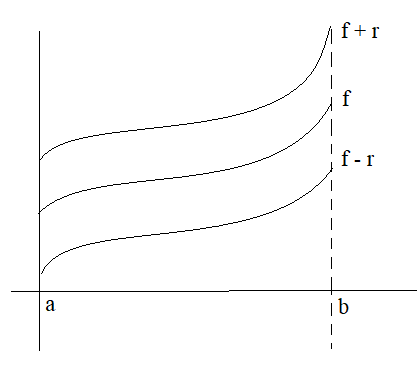
\includegraphics[width = 5cm]{lect2_1.png}
	$\overline{B}_r(f)$ состоит из тех непрерывных функций, графики которых содержатся в заштрихованном множестве.
\end{wrapfigure}
	
\textbf{Определение.} $(X, \rho)$ --- метрическое пространство, $A \subset X, x \in A.$
	
$x$ --- \textbf{внутренняя точка} $A \Leftrightarrow \exists \varepsilon > 0: B_{\varepsilon}(x) \subset A.$ 
	
$A$ называется \textbf{открытым} $\Leftrightarrow$ все его точки --- внутренние.
	
\textbf{Предложение 1}. Открытый шар $B_r(x)$ открыт.
	
\textbf{Доказательство.} Пусть $y \in B_r(x)$, т.е $\rho(y,x) < r.$
	
\begin{wrapfigure}{R}{0.3\textwidth}
	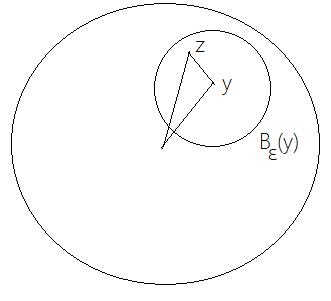
\includegraphics[width = 5cm]{lect2_2.png}
\end{wrapfigure}
	
Положим $\varepsilon = r - \rho(y,x).$
	
Покажем: $B_{\varepsilon}(y) \subset B_r(x). \quad (*)$
	
Пусть $z \in B_{\varepsilon}(y).$
	
Неравенство треугольника: $\rho(z, x) \leq \rho(z, y) + \rho(y, x)< \varepsilon + \rho(y, x) = r \Rightarrow z \in B_r(x) \Rightarrow \; (*)$ доказано $\Rightarrow B_r(x)$ открыто. 
	
\textbf{Предложение 2.} (1) $\varnothing$ открыто;
	
$\quad \quad \quad$ (2) $X$ открыто;
	
$\quad \quad \quad$ (3) $\{U_i\}_{i \in I}$ --- семейство открытых множеств в $X \Rightarrow \underset{i \in I}{\bigcup} U_i$ открыто.
	
$\quad \quad \quad$ (4) $U_1, U_2, ..., U_n \subset X$ открыты $\Rightarrow \underset{i = 1}{\overset{n}{\bigcap}} U_i$ открыто.
	
\textbf{Доказательство.} (1), (2) очевидны (из определения).
	
(3) $x \in \underset{i \in I}{\bigcup} U_i \Rightarrow \exists i_0 \in X\!\!: x \in U_{i_o} \Rightarrow \exists \varepsilon > 0\!\!: B_{\varepsilon}(x) \subset U_{i_0} \Rightarrow B_{\varepsilon}(x) \subset \underset{i \in I}{\bigcup} U_i.$
	
(4) достаточно для $n = 2.$
	
\begin{wrapfigure}{R}{0.3\textwidth}
	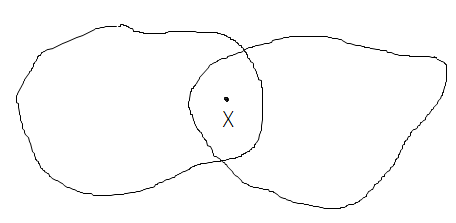
\includegraphics[width = 5cm]{lect2_3.png}
	$x \in U_1 \cap U_2$
\end{wrapfigure}
	
$\exists \varepsilon_1, \; \varepsilon_2 > 0\!\!: B_{\varepsilon_1}(x) \subset U_1, B_{\varepsilon_2} \subset U_2.$
	
Обозначим $\varepsilon = \min\{\varepsilon_1, \varepsilon_2\} \Rightarrow B_{\varepsilon}(x) \subset  U_1 \cap U_2.$
	
\section{Топологические пространства}
	
\textbf{Определение.} Пусть $X$ --- множество, $\tau \subset 2^{X}.$
	
\begin{wrapfigure}{R}{0.3\textwidth}
	Обозначение. $2^{X}$ --- множество всех подмножеств множества $X.$
\end{wrapfigure}

$\tau$ называется \textbf{топологией} на $X$, если
	
(1) $\varnothing \in \tau;$
	
(2) $X \in \tau;$
	
(3) $\{U_i\}_{i \in I}$ --- семейство множеств из $\tau \Rightarrow \underset{i \in I}{\bigcup} U_i \in \tau.$
	
(4) $U_1, ..., U_n \in \tau \Rightarrow \overset{n}{\underset{i = 1}{\bigcap}} U_i \in \tau.$
	
$\left(X, \tau \right)$ называется \textbf{топологическим пространством}.
	
Множества из $\tau$ называются \textbf{открытыми}.
	
\textbf{Наблюдение.} Из предложения 2: каждая метрика $\rho$ на множестве $X$ порождает топологию $\tau_{\rho}$ на $X.$
	
\textbf{Определение.} Топологическое пространство $(X, \tau)$ называется \textbf{метризуемым} $\Leftrightarrow \exists$ метрика $\rho\!\!: \; X\times X \to [0;\; +\infty)\!\!: \tau_{\rho} = \tau.$
	
\textbf{Замечание.} Если $\tau = \tau_{\rho},$ то такая $\rho$ не единственная! Например, $\tau_{\rho} = \tau_{2\rho}.$
	
\textbf{Пример-упражнение.} Метрики $\rho_1, \; \rho_2, \; \rho_{\infty}$ на $\mathbb{K}^n$ (где $\mathbb{K} = \mathbb{R}$ либо $\mathbb{C}$) порождают одну и ту же топологию на $\mathbb{K}^n.$
	
\textbf{Пример 1.} Дискретная топология
	
$X$ --- $\forall$ множество, $\tau = 2^X.$
	
Рассмотрим $\rho\!\!: X \times X \to [0; \; +\infty), \quad \rho(x,y) = \begin{cases} 1, \; \text{если } \; x \neq y, \\ 0 \text{ иначе.} \end{cases}$
	
Заметим: $\tau = \tau_{\rho}.$
	
Действительно: $B_1(x) = {x} \Rightarrow {x}$ открыто в $\tau_{\rho} \; \forall x \in X \Rightarrow$ каждое $A \subset X$ открыто в $\tau_{\rho}$, т.к. $A = \underset{x\in A}{\bigcup} {x} \Rightarrow \tau_{\rho} = \tau$ --- дискретная топология (метризуема).
	
\textbf{Пример 2}. Антидискретная топология
	
$X$ --- $\forall$ множество, $\tau = \{\varnothing, X\}.$
	
\textbf{Определение.} Пусть $\tau_1, \tau_2$ --- топологии на множестве $X.$
	
Говорят, что $\tau_1$ грубее $\tau_2$ ($\tau_2$ тоньше $\tau_1$), если $\tau_1 \subset \tau_2.$
	
Синонимы: грубее = слабее, тоньше = сильнее.
	
Дискретная топология --- самая тонкая, антидискретная --- самая грубая.
	
\textbf{Определение.} \textbf{Окрестность} точки $x$ в топологическом пространстве $X$ --- любое открытое множество $U \subset X$, содержащее $x.$
	
\textbf{Определение.} Топологическое пространство $X$ называется \textbf{хаусдорфовым} $\Leftrightarrow \forall x, y \in X, \; x \neq y, \; \exists$ окрестности $U \ni x, V \ni y\!\!: U \cap V = \varnothing.$
	
\textbf{Предложение.} Метризуемое топологическое пространство хаусдорфово.
	
\textbf{Доказательство.} Пусть $(X, \rho)$ --- метрическое пространство, $x, y \in X, \; x \neq y$. Обозначим $a = \rho(x, y), \; a > 0.$
	
\begin{wrapfigure}{R}{0.3\textwidth}
	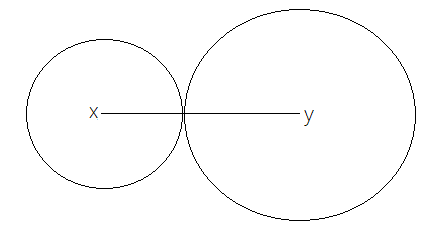
\includegraphics[width = 5cm]{lect2_4.png}
	Из неравенства треугольника: $B_{\frac{a}{2}}(x) \cap B_{\frac{a}{2}}(y) = \varnothing.$
\end{wrapfigure}
	
\textbf{Следствие.} Антидискретная топология на множестве, содержащем более одного элемента, неметризуема (т.к. неухаусдорфова).
	
\textbf{Определение.} Пусть $X$ --- топологическое пространство.
	
Множество $F \subset X$ называется \textbf{замкнутым} $\Leftrightarrow X \backslash F$ открыто.
	
\textbf{Предложение.} Пусть $X$ --- топологическое пространство, $\tau' = \{ F \subset X\!\!: F \text{ замкнуто}\}$. Тогда:
	
(1) $\varnothing \in \tau';$
	
(2) $x \in \tau';$
	
(3) $\{F_i\}$ - семейство множеств из $\tau' \Rightarrow \bigcap_{i \in I} F_i \in \tau';$
	
(4) $F_1, F_2, ..., F_n \in \tau' \Rightarrow \bigcup^n_{i = 1} F_i$ замкнуто.
	
\begin{wrapfigure}{R}{0.3\textwidth}
	Напоминание:
		
	$X \backslash \bigcap_{i \in I} F_i = \bigcup_{i \in I}\left( X \backslash F_i \right);$
		
	$X \backslash \bigcup_{i \in I} F_i = \bigcap_{i \in I}\left( X \backslash F_i \right).$
\end{wrapfigure}
	
	
\textbf{Наблюдение.} Если $X$ --- множество, $\tau' \subset 2^X$ удовлетворяет (1)-(4) из предложения $\Rightarrow \{X \backslash F \colon F \in \tau'\}$ --- топология на $X.$
	
\textbf{Пример.} Топология Зарисского
	
$X$ --- множество, $\mathbb{K} = \mathbb{R}$ или $\mathbb{C}$.
	
\textbf{Определение.} $A \subset \mathbb{K}^X$ --- \textbf{подалгебра} в $\mathbb{K}^X,$ если
	
(1) $A$ --- векторное подпространство в $\mathbb{K}^X;$
	
(2) $1 \in A$ (где 1 -- функция, тождественно равная единице);
	
(3) $f, g \in A \Rightarrow fg \in A$ ($fg$ --- поточечное произведение $f$ и $g$).
	
Зафиксируем какую-либо подалгебру $A \subset \mathbb{K}^X.$
	
$\forall S \subset A$ обозначим $V(S) = \{ x \in X: \; \forall f \in S \; f(x) = 0 \}$ 
	
\textbf{Упражнение.} На $X$ существует топология, в которой $F \subset X$ замкнуто $\Leftrightarrow F = V(S)$ для некоторого $S \subset A$. Она называется \textbf{топологией Зарисского.}
	
\textbf{Важный частный случай:} $X = \mathbb{K}^n, \; A = \mathbb{K}[t_1, ..., t_n].$

\textbf{Упражнение.} Описать топологию Зарисского в явном виде для следующих случаев:
	
(1) $X$ --- любое множество, $A = \mathbb{K}^X;$
	
(2) $X = \mathbb{K}, \; A = \mathbb{K}[t];$
	
(3) $X = [a, b] \subset \mathbb{R}, \; A = C[a,b].$

\section{Открытое множество в метрическом пространстве}

$(X, \rho)$ --- метрическое пространство, $x \in X, \; r \geq 0$.

\textbf{Определение.} Открытый шар с центром в $x$ радиуса $r$ --- это 
$B_r(x) = \{ y \in X\!\!: \rho(y, x) < r\}$ --- r-окрестность x. 

\textbf{Замкнутый шар} с центром в $x$ радиуса $r$ --- это
$\overline{B}_r(x) = \{y \in X\!\!: \rho(y, x) \leq r\}.$

\textbf{Пример.} $x = \mathbb{R} \Rightarrow B_r(x) = (x - r, x + r); \quad \overline{B}_r(x) = [x - r, \; x + r].$

\textbf{Упражнение.} Нарисовать $B_1(o)$ на $(\mathbb{R}^2, \rho_p)$ для $p = 1, p = 2, p = \infty$ (для $p = 2$ --- круг, для $p = 3$ --- шар, как в школе).

\textbf{Пример.} $X = C[a,b]$ с равномерной метрикой.

\begin{wrapfigure}{R}{0.3\textwidth}
	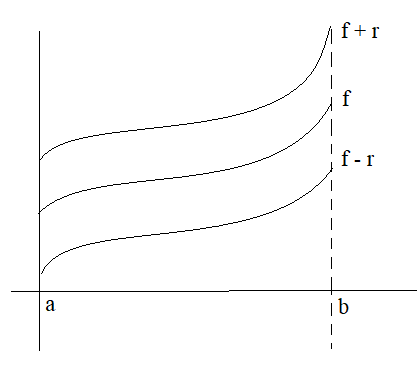
\includegraphics[width = 5cm]{lect2_1.png}
	$\overline{B}_r(f)$ состоит из тех непрерывных функций, графики которых содержатся в заштрихованном множестве.
\end{wrapfigure}

\textbf{Определение.} $(X, \rho)$ --- метрическое пространство, $A \subset X, x \in A.$
$x$ --- \textbf{внутренняя точка} $A \Leftrightarrow \exists \varepsilon > 0: B_{\varepsilon}(x) \subset A.$ 

$A$ называется \textbf{открытым} $\Leftrightarrow$ все его точки --- внутренние.

\textbf{Предложение 1}. Открытый шар $B_r(x)$ открыт.

\textbf{Доказательство.} Пусть $y \in B_r(x)$, т.е $\rho(y,x) < r.$ 

\begin{wrapfigure}{R}{0.3\textwidth}
	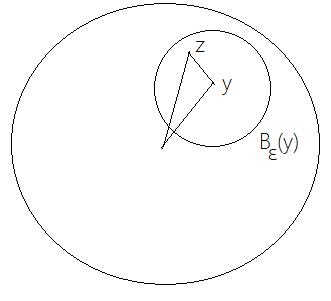
\includegraphics[width = 5cm]{lect2_2.png}
\end{wrapfigure}

Положим $\varepsilon = r - \rho(y,x).$

Покажем: $B_{\varepsilon}(y) \subset B_r(x). \quad (*)$

Пусть $z \in B_{\varepsilon}(y).$

Неравенство треугольника: $\rho(z, x) \leq \rho(z, y) + \rho(y, x)< \varepsilon + \rho(y, x) = r \Rightarrow z \in B_r(x) \Rightarrow \; (*)$ доказано $\Rightarrow B_r(x)$ открыто. 

\textbf{Предложение 2.} (1) $\varnothing$ открыто;

$\quad \quad \quad$ (2) $X$ открыто;

$\quad \quad \quad$ (3) $\{U_i\}_{i \in I}$ --- семейство открытых множеств в $X \rightarrow \underset{i \in I}{\bigcup} U_i$ открыто.

$\quad \quad \quad$ (4) $U_1, U_2, ..., U_n \subset X$ открыты $\Rightarrow \underset{i = 1}{\overset{n}{\bigcap}} U_i$ открыто.

\textbf{Доказательство.} (1), (2) очевидны (из определения).

(3) $x \in \underset{i \in I}{\bigcup} U_i \Rightarrow \exists i_0 \in X\!\!: x \in U_{i_0} \Rightarrow \exists \varepsilon > 0\!\!: B_{\varepsilon}(x) \subset U_{i_0} \Rightarrow B_{\varepsilon}(x) \subset \underset{i \in I}{\bigcup} U_i.$

(4) достаточно для $n = 2$

\begin{wrapfigure}{R}{0.3\textwidth}
	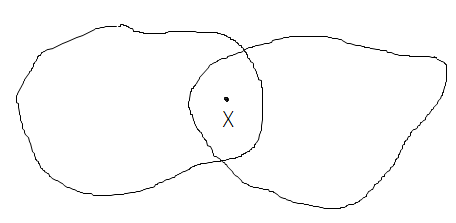
\includegraphics[width = 5cm]{lect2_3.png}
	$x \in U_1 \cap U_2$
\end{wrapfigure}

$\exists \varepsilon_1, \; \varepsilon_2 > 0\!\!: B_{\varepsilon_1}(x) \subset U_1, B_{\varepsilon_2} \subset U_2.$

Обозначим $\varepsilon = \min\{\varepsilon_1, \varepsilon_2\} \Rightarrow B_{\varepsilon}(x) \subset  U_1 \cap U_2.$

\section{Топологические пространства}

\textbf{Определение.} Пусть $X$ --- множество, $\tau \subset 2^{X}.$

\begin{wrapfigure}{R}{0.3\textwidth}
	Обозначение. $2^{X}$ --- множество всех подмножеств множества $X.$
\end{wrapfigure}

$\tau$ называется \textbf{топологией} на $X$, если

(1) $\varnothing \in \tau;$

(2) $X \in \tau;$

(3) $\{U_i\}_{i \in I}$ --- семейство множеств из $\tau \Rightarrow \underset{i \in I}{\bigcup} U_i \in \tau.$

(4) $U_1, ..., U_n \in \tau \Rightarrow \underset{i = 1}{\overset{n}{\bigcap}} U_i \in \tau.$

$\left(X, \tau \right)$ называется \textbf{топологическим пространством}.

Множества из $\tau$ называются \textbf{открытыми}.

\textbf{Наблюдение.} Из предложения 2: каждая метрика $\rho$ на множестве $X$ порождает топологию $\tau_{\rho}$ на $X.$

\textbf{Определение.} Топологическое пространство $(X, \tau)$ называется \textbf{метризуемым} $\Leftrightarrow \exists$ метрика $\rho\!\!: \; X\times X \to [0;\; +\infty)\!\!: \tau_{\rho} = \tau.$

\textbf{Замечание.} Если $\tau = \tau_{\rho},$ то такая $\rho$ не единственная! Например, $\tau_{\rho} = \tau_{2\rho}$

\textbf{Пример-упражнение.} Метрики $\rho_1, \rho_2, \rho_{\infty}$ на $\mathbb{K}^n$ (где $\mathbb{K} = \mathbb{R}$ либо $\mathbb{C}$) порождают одну и ту же топологию на $\mathbb{K}^n.$

\textbf{Пример 1.} Дискретная топология

$X$ --- $\forall$ множество, $\tau = 2^X.$

Рассмотрим $\rho\!\!: X \times X \to [0; \; +\infty), \quad \rho(x,y) = \begin{cases} 1, \text{если } \; x \neq y, \\ 0 \text{ иначе.} \end{cases}$

Заметим: $\tau = \tau_{\rho}.$

Действительно: $B_1(x) = {x} \Rightarrow {x}$ открыто в $\tau_{\rho} \; \forall x \in X \Rightarrow$ каждое $A \subset X$ открыто в $\tau_{\rho}$, т.к. $A = \bigcup_{x\in A} {x} \Rightarrow \tau_{\rho} = \tau$ --- дискретная топология (метризуема).

\textbf{Пример 2}. Антидискретная топология

$X$ ---fа $\forall$ множество, $\tau = \{\varnothing, X\}.$

\textbf{Определение.} Пусть $\tau_1, \tau_2$ --- топологии на множестве $X.$

Говорят, что $\tau_1$ грубее $\tau_2$ ($\tau_2$ тоньше $\tau_1$), если $\tau_1 \subset \tau_2.$

Синонимы: грубее = слабее, тоньше = сильнее.

Дискретная топология --- самая тонкая, антидискретная --- самая грубая.

\textbf{Определение.} \textbf{Окрестность} точки $x$ в топологическом пространстве $X$ --- любое открытое множество $U \subset X$, содержащее $x.$

\textbf{Определение.} Топологическое пространство $X$ называется \textbf{хаусдорфовым} $\Leftrightarrow \forall x, y \in X, x \neq y, \exists$ окрестности $U \ni x, V \ni y: U \cap V = \varnothing.$

\textbf{Предложение.} Метризуемое топологическое пространство хаусдорфово.

\textit{Доказательство.} Пусть $(X, \rho)$ --- метрическое пространство, $x, y \in X, x \neq y$. Обозначим $a = \rho(x, y), \; a > 0.$

\begin{wrapfigure}{R}{0.3\textwidth}
	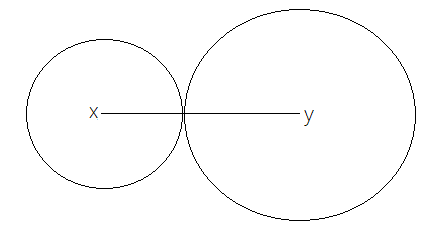
\includegraphics[width = 5cm]{lect2_4.png}
	Из неравенства треугольника: $B_{\frac{a}{2}}(x) \cap B_{\frac{a}{2}}(y) = \varnothing.$
\end{wrapfigure}

\textit{Следствие.} Антидискретная топология на множестве, содержащем более одного элемента, неметризуема (т.к. неухаусдорфова).

\textbf{Определение.} Пусть $X$ --- топологическое пространство.

Множество $F \subset X$ называется \textbf{замкнутым} $\Leftrightarrow X \backslash F$ открыто.

\textbf{Предложение.} Пусть $X$ --- топологическое пространство, $\tau' = \{ F \subset X: F \text{замкнуто}\}$. Тогда:

(1) $\varnothing \in \tau';$

(2) $x \in \tau';$

(3) $\{F_i\}$ - семейство множеств из $\tau' \Rightarrow \bigcap_{i \in I} F_i \in \tau';$

(4) $F_1, F_2, ..., F_n \in \tau' \Rightarrow \bigcup^n_{i = 1} F_i$ замкнуто.

\begin{wrapfigure}{R}{0.3\textwidth}
	Напоминание:
	
	$X \backslash \bigcap_{i \in I} F_i = \bigcup_{i \in I}\left( X \backslash F_i \right);$
	
	$X \backslash \bigcup_{i \in I} F_i = \bigcap_{i \in I}\left( X \backslash F_i \right).$
\end{wrapfigure}


\textbf{Наблюдение.} Если $X$ --- множество, $\tau' \subset 2^X$ удовлетворяет (1)-(4) из предложения $\Rightarrow \{X \backslash F \colon F \in \tau'\}$ --- топология на $X.$

\textbf{Пример.} Топология Зарисского

$X$ --- множество, $\mathbb{K} = \mathbb{R}$ или $\mathbb{C}$.

\textbf{Определение.} $A \subset \mathbb{K}^X$ - \textbf{подалгебра} в $\mathbb{K}^X,$ если

(1) $A$ --- векторное подпространство в $\mathbb{K}^X;$

(2) $1 \in A$ (где 1 --- функция, тождественно равная единице);

(3) $f, g \in A \Rightarrow fg \in A$ ($fg$ --- поточечное произведение $f$ и $g$).

Зафиксируем какую-либо подалгебру $A \subset \mathbb{K}^X.$

$\forall S \subset A$ обозначим $V(S) = \{ x \in X: \; \forall f \in S \; f(x) = 0 \}$ 

\textbf{Упражнение.} На $X$ существует топология, в которой $F \subset X$ замкнуто $\Leftrightarrow F = V(S)$ для некоторого $S \subset A$. \\Она называется \textbf{топологией Зарисского.}

Важный частный случай: $X = \mathbb{K}^n, \; A = \mathbb{K}[t_1, ..., t_n].$

\textbf{Упражнение.} Описать топологию Зарисского в явном виде для следующих случаев:

(1) $X$ --- любое множество, $A = \mathbb{K}^X;$

(2) $X = \mathbb{K}, \; A = \mathbb{K}[t];$

(3) $X = [a, b] \subset \mathbb{R}, \; A = C[a,b].$

\section{База и предбаза топологии}

\textbf{Лемма.} X --- множество, $\beta \subset 2^{X}.$ Следующие свойства множества $A \subset X$ эквиваленты: 

\begin{wrapfigure}{R}{0.3\textwidth}
	
	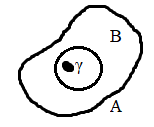
\includegraphics[width = 5cm]{lect3_1.png}
	
	$\gamma \subset 2^X$
	
	Обозначение: $\bigcup_{C \in \gamma} C = \cup \gamma$
\end{wrapfigure}

$(1) \; \exists \gamma \subset \beta$ т.ч. $A = \cup \gamma;$

$(2) \; \forall x \in A \; \exists B \in \beta$ т.ч. $x \in B \subset A.$ 

\textbf{Доказательство.} $(1) \Rightarrow (2).$ Пусть $A = \cup \gamma, \gamma \subset \beta, x \in A \Rightarrow \exists B \in \gamma: x \in B \Rightarrow$ B удовлетворяет (2). 

$(2) \Rightarrow \forall x \in A \; \exists B_{1} \in \beta: x \in B_{1} \subset A \Rightarrow \gamma = \{B_{x}: x \in A\}$ удовлетворяет (1). 

\textbf{Определение.} $(x, \tau)$ --- топологическое пространство. 

$(1) \; \beta \in \tau$ --- база $\tau$ (или база $(X, \tau)) \Leftrightarrow$ каждое $U \in \tau$ является объединением некоторого подсемейства в $\beta \Leftrightarrow \forall U \in \tau \; \forall x \in U \; \exists B \in \beta$ т.ч. $x \in B \subset U.$ 

$(2) \; \sigma \subset \tau$ --- предбаза $\tau$ (предбаза $(x, \tau)$ --- из леммы) $\Leftrightarrow$ семейство $\{U_{1} \cap ... \cap U_{n}: U_{i} \in \sigma, \; n \in \mathbb{N}\}$ --- база $\tau.$ 

\textbf{Пример.} $(x, \rho)$ --- метрическое пространство $\Leftrightarrow \{B_{r}(x): x \in X, r > 0\}$ --- база $\tau_{p}.$

\textbf{Пример.} $X = \mathbb{R}, \; \sigma = \{(-\infty, b); (a, +\infty): a, b \in \mathbb{R}\}$ --- предбаза $\mathbb{R},$ но не база. 

\textbf{Предложение.} X --- множество, $\beta, \sigma \subset 2^{X}.$

(1) На X $\exists$ топология с базой $\beta \Leftrightarrow$ $\begin{cases} 
	(a) \cup \beta = X \\
	(b) \forall B_{1}, B_{2} \in \beta \; \forall x \in B_{1} \cap B_{2} \; \exists B_{3} \in \beta: \\ x \in B_{3} \subset B_{1} \cap B_{2}.
\end{cases}$

(2) На X $\exists$ топология с предбазой $\sigma \Leftrightarrow \cup \sigma = X.$ 

\begin{wrapfigure}{R}{0.3\textwidth}
	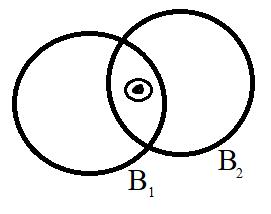
\includegraphics[width = 5cm]{lect3_2.png}
\end{wrapfigure}

\textbf{Доказательство.} (1) $(\Leftarrow)$ следует из открытости X и $B_{1} \cap B_{2}.$ 

$\Rightarrow$ Обозначим $\tau = \{\cup \gamma: \gamma \in \beta\}.$ Покажем, что $\tau$ --- топология на X. 

$\varnothing = \cup \varnothing \in \tau; \; X = \cup \beta \in \tau;$ объединение множеств из $\tau$ принадлежит $\tau.$

Пусть $U_{1}, U_{2} \in \tau.$ Хотим: $U_{1} \cap U_{2} \in \tau.$

Пусть $x \in U_{1} \cap U_{2} \xRightarrow{\text{из леммы}}$ $\exists B_{1}, B_{2} \in \beta$ т.ч. $x \in B_{k} \subset U_{k} (k = 1, 2) \Rightarrow x \in B_{1} \cap B_{2} \Rightarrow^{(b)} \Rightarrow \exists B_{3} \in \beta$ т.ч. $x \in B_{3} \subset B_{1} \cap B_{2} \subset U_{1} \cap U_{2} \xRightarrow{\text{из леммы}} U_{1} \cap U_{2} \in \tau \Rightarrow \tau$ --- топология на X, $\beta$ --- ее база. 

(2) $(\Rightarrow)$ из открытости X. 

$(\Leftarrow)$ cемейство $\{U_{1} \cap ... \cap U_{n}: U_{i} \in \sigma, n \in \mathbb{B}\}$ удовлетворяет (a), (b) $\Rightarrow$ оно --- база топологии, а $\sigma$ --- ее предбаза. 
	
\textbf{Пример.} Топология поточечной сходимости

\begin{wrapfigure}{R}{0.3\textwidth}
	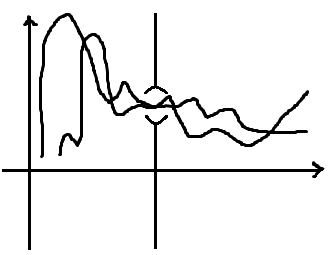
\includegraphics[width = 5cm]{lect3_3.png}
\end{wrapfigure}

Пусть $\mathbb{K} = \mathbb{R}$ или $\mathbb{C}, \; S \subset \mathbb{K}^{X},$ где $X - \forall$ множество) 
	
$\forall x \in X, \forall$ интервала $I \subset \mathbb{R}$ обозначается $G(x, I) = \{f \in S: f(x) \in I\}.$ 
	
Семейство $\{G(x, I): x \in X, I \subset R$ --- интервал (для $\mathbb{K} = \mathbb{C}$ --- открытый круг)\} является предбазой некоторой топологии на S. Она называется \textbf{топологией поточечной сходимости} на S. 

\section{Сходимость последовательностей в топологическом пространстве}

(Окрестность точки --- это любое открытое множество, содержащее эту точку)

X --- топологическое прространство, $x \in X, (x_{n})$ --- последовательность в X. 

\textbf{Опредедение.} $(x_{n})$ сходится к $x$ ($x$ является пределом $(x_{n}) \Leftrightarrow \forall$ окрестности $U \ni x \; \exists N \in \mathbb{N} \; \forall n \geq N \; x_{n} \in U.$

\textbf{Обозначение.} $x_{n} \to x (n \to \infty),$ или $x = \underset{n \to \infty}{\lim} x_{n}.$ 

\textbf{Определение.} (1) Семейство $\beta_{x}$ окрестностей точки $x \in X$ --- база окрестностей x (база в x) $\Rightarrow \forall$ окрестности $U \in$ (знак наоборот) $\exists V \in \beta_{x}, V \subset U.$

(2) Семейство $\sigma_{1}$ окрестностей точки $x \in X$ ---- предбаза окрестностей x (предбаза в x). 

$\Leftrightarrow \{U_{1} \cap ... \cap... U_{n}: U_{i} \in \sigma_{x}, n \in \mathbb{N}\}$ --- база в x. 

\textbf{Пример.} $(x, \rho)$ --- метрическое пространство. 

\begin{wrapfigure}{R}{0.3\textwidth}
	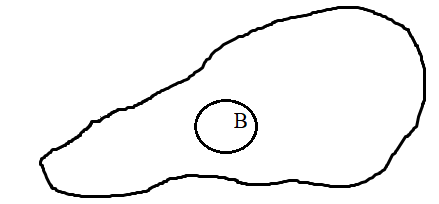
\includegraphics[width = 5cm]{lect3_4.png}
\end{wrapfigure}

$\{B_{r}(x): r > 0\}$ --- база в x. 

$\{B_{\frac{1}{n}}(x): n \in \mathbb{N}\}$ --- тоже (важный пример, запомнить.)

\textbf{Предложение.} X --- топологическое пространство, $x \in X, \sigma_{x}$ --- предбаза в x, $(x_{n})$ --- последовательность в X.

$x_{n} \to x \; (n \to \infty) \Leftrightarrow \forall V \in \sigma_{x} \; \; \exists N \in \mathbb{N} \; \forall n \geq N \; x_{n} \in V.$

\textbf{Доказательство.} $(\Leftarrow)$ Пусть U --- окрестность x $\Rightarrow \exists V{1}, ..., V_{p} \in \sigma_{x}$ т.ч. $V_{1} \cap ... \cap V_{p} \subset U.$ 

$\exists N_{1}, ..., N_{p}$ т.ч. $\forall n \geq N_{i} \; x_{n} \in V_{i} \; (i = 1, ..., p).$

Обозначим $N = \underset{1 \leq i \leq n}{\max} N_{i} \Rightarrow \forall n \geq N \; x_{n} \in V_{1} \cap ... \cap V_{p} \subset U.$ 


\textbf{Следствие.} $(x, \rho)$ --- метрическое пространство, $x \in X, (x_{n})$ --- последовательность в X. Следующие утверждения эквивалентны: 

$(1) \; x_{n} \to x;$

$(2) \; \forall$ открытого щара V с центром в x $\exists N \in \mathbb{N} \; \forall n \geq N\; x_{n} \in V;$

$(3) \; \forall \varepsilon > 0 \quad \exists N \in \mathbb{N} \quad \forall n \geq N \quad \rho(x_{n}, x) < \varepsilon;$

$(4) \; \rho(x_{n}, x) \to 0.$

\textbf{Предложение.} X --- хаусдорфово топологического пространство, $(x_{n})$ --- последовательность в X, $x_{n} \to x \in X, \; x_{n} \to y \in X \Rightarrow x = y.$ 

\textbf{Доказательство.} Пусть $x \neq y \Rightarrow \exists$ окрестности $U \ni x$, $V \ni y, \; U \cap V = \varnothing.$

Из $\exists N_{1}$ т.ч. $\forall n \geq N_{1} x_{n} \in U$ и $\exists N_{2}$ т.ч. $\forall n \geq N_{2} \; x_{n} \in V$ следует, что $x_{n} \in U \cap V \; \forall n \geq \max\{{N_{1}, N_{2}}\}$ --- противоречие. 

\textbf{Пример.} X --- антидискретное пространство. Каждая последовательность в X сходится к каждой точке $x \in X.$ 

\textbf{Пример.} X --- дискретное топологическое пространство $x_{n} \to x \Leftrightarrow \exists N \in \mathbb{N} \; \forall n \geq N \; \; x_{n} = x.$ 

Действительно: $(\Rightarrow) \; {x}$ --- окрестность x. Далее см. определение сходимости. 

\textbf{Пример-упражнение.} $\mathbb{K} = \mathbb{R}$ или $\mathbb{C}, X$ --- множество, $S \subset \mathbb{K}^{X}.$

Пусть $f_{n} \to F$ в $S$ с топологией поточечной сходимости $\Leftrightarrow \forall x \in X \; f_{n}(x) \to f(x).$

\section{Замыкание, внутренность, граница} 

\subsection{Замыкание} 

X --- топологическое пространство, $A \subset X.$ 

\textbf{Определение.} Замыкание A --- множество $\overline{A} = \cap\{F \subset X: F$ замкнуто, $A \subset F\}.$ 

\textbf{Наблюдение.} $\overline{A}$ --- наименьшее замкнутое множество, содержащее A. В частности, если A замкнуто, то $A = \overline{A}.$ 

\textbf{Предложение.} $(1) \; A \subset B \subset X \Rightarrow \overline{A} \subset \overline{B};$

$(2) \; \overline{\overline{A}} = \overline{A};$ 

$(3) \; \overline{A \cup B} = \overline{A} \cup \overline{B}.$

\textbf{Доказательство.} (1) из определения, (2) из наблюдения, (3) $A \subset A \cup B \xRightarrow{(1)} \overline{А} \subset \overline{A \cup B}.$ Аналогично $\overline{B} \subset \overline{A \cup B} \Rightarrow \overline{A} \cup \overline{B} \subset \overline{A \cup B}.$

$A \cup B \subset \overline{A} \cup \overline{B} \xRightarrow{(1)} \overline{A \cup B} \subset \overline{\overline{\overline{А} \cup \overline{B}}} = \overline{A} \cup \overline{B},$ т.к. $\overline{A} \cup \overline{B}$ замкнуто.

\textbf{Предложение.} $x \in \overline{A} \Leftrightarrow$ окрестности $U \ni x, \; U \cap A \neq \varnothing.$ 

\textbf{Доказательство.} $x \notin \overline{A} \Leftrightarrow \exists$ замкнутое $F \subset X$ т.ч. $F \supset A, \; x \notin F \; \xLeftrightarrow{U = X\backslash F} \exists x \in U$ и $\exists$ открытое $U \subset X$ т.ч. $U \cap A = \varnothing \Leftrightarrow \exists$ окрестность $U \ni x, \; U \cap A = \varnothing.$

\textbf{Определение.} X --- топологическое пространство, $A \subset X.$ Тогда $x \in X$ --- \textbf{предельная точка} A $\Leftrightarrow \; x \in \overline{A\backslash{\{x\}}} \xLeftrightarrow{\text{предложение}}$ в каждой окрестности x есть точки из A, отличные от x. 

\textbf{Обозначение.} $A' = \{x \in X | x$ --- предельная точка A\} --- производное множество множества A.

Из предложения $\overline{A} = A \cup A'.$ В частности: A замкнуто $\Leftrightarrow A' \subset A.$ 

\textbf{Определение.} $x \in A$ --- \textbf{изолированная точка} A $\Leftrightarrow x \in A \backslash A' \Leftrightarrow \exists$ окрестность $U \ni x$ т.ч. $U \cap A = \{x\}.$ 

$\overline{A} = A' \sqcup$ {изолированные точки A}.

\subsection{Внутренность}

X --- топологическое пространство, $A \subset X.$ 

\textbf{Определение.} \textbf{Внутренность} A --- это Int(A) = $\bigcup \{U \subset X\!\!\!: U$ открыто, $U \subset A\}.$ 

\textbf{Наблюдение.} (1) Int A --- наибольшее открытое множество, содержащееся в A. В частности: A открытое $\Leftrightarrow$ A = Int A. 

$\quad \quad \quad \quad \quad \quad \; \;$ (2) Если $(X, \; \rho)$ --- метрическое пространство, то $x \in \text{Int} A \Leftrightarrow \exists \varepsilon > 0$ т.ч. $B_{\varepsilon}(x) \subset A.$ 

\textbf{Упражнение.} Int A = $X \backslash \overline{(X \backslash A)}; \quad \overline{A} = X \backslash \text{Int}(X \backslash A).$

\fbox{Int A $\subset A \subset \overline{A}$}

\textbf{Определение.} \textbf{Граница} A --- это $\Delta A = \overline{A} \backslash$Int A. 

\textbf{Наблюдение.} $x \in \delta \; A \Leftrightarrow \forall$ окрестностей $U \ni x \; U\cap A \neq \varnothing, \; U \cap (X \backslash A) \neq \varnothing.$

\textbf{Примечание 1.} $X = \mathbb{R}, A = \mathbb{Z} \Rightarrow \overline{A} = \mathbb{Z},$ Int $A = \varnothing, \; \delta A = A = \mathbb{Z},$ все точки A изолированы, $A' = \varnothing.$ 

\textbf{Примечание 2.} $X = \mathbb{R}, A = (0, 1) \Rightarrow \overline{A} = [0, 1],$ Int A = A = (0, 1), $\delta A = \{0, 1\},$ изолированных точек нет, $A' = [0, 1].$

\textbf{Примечание 3.} $X = \mathbb{R}, A = \{\dfrac{1}{n}: n \in \mathbb{N}\} \cup \{0\ \Rightarrow \overline{A} = A$ (т.к. $\mathbb{R} \backslash A = (-\infty, 0) \cup (1, +\infty) \cup (\bigcup^{\infty}_{n = 1} (\dfrac{1}{n + 1}, \dfrac{1}{n})).$ Int $A = \varnothing, \; \delta A = A,$ \{изолированные точки A\} = $\{\dfrac{1}{n}: n \in \mathbb{N}\}; \{0\} = A'.$ 

\textbf{Определение.} X --- топологическое пространство. Множество $A \subset X$ \textbf{плотно} в X (= \textbf{всюду плотно} в X) $\Leftrightarrow \overline{A} = X.$ 

\textbf{Наблюдение.} A плотно в X $\Leftrightarrow \forall x \in X \forall$ окрестности $U \ni x \; U \cap A \neq \varnothing \Leftrightarrow \forall$ непустого открытого $U \subset X \; U \cap A \neq \varnothing.$ 

\textbf{Определение.} X \textbf{сепарабельно} $\Leftrightarrow \; \exists$ не более чем счетное плотное подмножество в X. 

\textbf{Пример 1.} Дискретное пространство сепарабельно $\Leftrightarrow$ оно само не более чем счетно. 

\textbf{Пример 2.} Антидискретное пространство сепарабельно (каждое непустое подмножество плотно). 

\textbf{Пример 3.} $\mathbb{R}$ сепарабельно (т.к. $\mathbb{Q}$ плотно в $\mathbb{R}$). 

\textbf{Пример-упражнение 4.} $\mathbb{R}^n, \mathbb{C}^n, l^{1}, l^{2}$ сепарабельны, $l^{\infty}$ несепарабельно. 

\textbf{\textit{Мое} доказательство.} Из доказанного мною выше (см. первая лекция) $l^{2}$ --- векторное пространство в $\mathbb{K}^{N},$ норма на $l^2\!\!: ||x||_{2} = \sqrt{\underset{i = 1}{\overset{\infty}{\sum}}|x_{i}|^2}.$ 

Теперь найдем в $l^{2}$ \textit{счетное всюду плотное множество}. 

Пусть L --- множество всех последовательностей с рациональными членами, у которых только конечное число членов не равно нулю, а остальные члены нулевые. 

Покажем, что $L$ --- искомое. 

1) Т.к. L --- объединение счетного числа счетных множеств, \textit{L счетно};

2) Теперь покажем, что L всюду плотно в $l^{2},$ то есть что в любом шаре $B_{\varepsilon}(x) \in l^{2},$ где $x \in l^{2}, \; \varepsilon > 0$ --- произвольное, найдется точка $r$ из $L: \; \underset{i = 1}{\overset{\infty}{\sum}}|x_{i} - r_{i}|^2 < \varepsilon.$ 

Возьмем в $l^{2}$ последовательность $\{x_{n}\}.$ Тогда ряд $\underset{i = 1}{\overset{\infty}{\sum}}|x_{i}|^2$ сходится. Это значит, что $\underset{n \to \infty}{\lim} \overset{\infty}{\underset{k = N + 1}{\sum}}|x_{k}|^{2} = 0,$ то есть, начиная с некоторого $N,$ $\overset{\infty}{\underset{k = N + 1}{\sum}}|x_{k}|^{2} < \dfrac{\varepsilon^{2}}{2},$ где $\varepsilon > 0$ --- произвольное. 

Множество рациональных чисел всюду плотно в множестве действительных. Это значит, что если зафиксируем $\varepsilon > 0$ и рассмотрим каждый интервал $(x_{i} - \dfrac{\varepsilon}{\sqrt{2N}}, x_{i} + \dfrac{\varepsilon}{\sqrt{2N}}),$ то в любом из них мы сможем найти некоторое рациональное число $r$ (конечно, для каждого $i$ --- свое $r$). Перепишем это: $|x_{i} - r| < \dfrac{\varepsilon}{\sqrt{2N}}.$ Возведем обе части неравенства в квадрат, так как они неотрицательные. Получим $|x_{i} - r|^{2} < \dfrac{\varepsilon^{2}}{2N}.$

Тогда расстояние между $x \in l^{2}, \; r \in \mathbb{Q} \; = \sqrt{\sum\limits_{i = 1}^{\infty} |x_{i} - r|^{2}}$ = 

= $\sqrt{\sum\limits_{i = 1}^{N} |x_{i} - r|^{2} + \sum\limits_{i = N + 1}^{\infty} |x_{i}|^{2}} < \sqrt{\frac {N \cdot \varepsilon^{2}}{2N} + \frac {\varepsilon^{2}}{2}} = \varepsilon \Rightarrow r \in B_{\varepsilon}(x).$

Значит, $L$ \textit{всюду плотно} в $l^{2}.$ Тогда $L$ --- искомое. Значит, $l^{2}$ сепарабельно. Что и требовалось доказать. $\square$ 

\section{Аксиомы счетности}

X --- топологическое пространство. 

\textbf{Определение.} (1) X удовлетворяет \textbf{1-ой аксиоме счетности} $\Leftrightarrow \forall x \in X \exists$ не более чем счетная база окрестностей x.

$\quad \quad \quad \quad \quad \quad \quad \;(2) \; X$ удовлетворяет \textbf{2-ой аксиоме счетности} (является пространством со \textbf{счетной базой}) $\Leftrightarrow \exists$ не более чем счетная база топологии на X. 

\textbf{Предложение.} X удовлетворяет 2-ой аксиоме счетности $\Rightarrow$ X удовлетворяет 1-ой аксиоме счетности. 

\textbf{Доказательство.} Пусть $\beta$ --- не более чем счетная база топологии на X. $x \in X;$ тогда $\{U \in \beta: \; U \ni x\}$ --- база окрестностей x. 

\textbf{Пример 1.} X --- метризуемо $\Rightarrow$ X удовлетворяет 1-ой аксиоме счетности. Действительно, $\forall x \in X \; \{B_{\frac{1}{n}}(x): \; n \in \mathbb{N}\}$ --- база окрестностей x. 

\textbf{Определение.} Семейство $\beta_{x}$ окрестностей точки $x \in X$ --- \textbf{база окрестностей x} $\Leftrightarrow \forall$ окрестности $U \ni x \; \exists V \in \beta_{x}, \; V \subset U.$

\textbf{Пример 2.} Дискретное пространство X удовлетворяет 1-ой аксиоме счетности. Оно удовлетворяет 2-ой аксиоме счетности $\Leftrightarrow$ оно не более чем счетно. 

\textbf{Пример 3.} $\mathbb{R}$ удовлетворяет 2-ой аксиоме счетности. А именно, $\{(a, b)\!\!: a < b, \quad a, \; b \in \mathbb{Q}\}$ --- база $\mathbb{R}.$ Действительно, $\forall c, d \in \mathbb{R}, \; c < d,$ выполнено $(c, d) = \bigcup\{(a, b): a, b \in \mathbb{Q}, \; c < a < b < d\}$ --- в силу плотности $\mathbb{Q}$ в $\mathbb{R}.$ 

\textbf{Предложение.} Топологическое пространство со счетной базой сепарабельно. 

\textbf{Доказательство.} $\{U_{n}\!\!: \; n \in \mathbb{N}\}$ --- счетная база в X; $U_{n} \neq \varnothing \quad \forall n$ (если пусто, можно выкинуть и ничего не потерять). $\forall n \in \mathbb{N}$ выберем $x_{n} \in U_{n} \Rightarrow \{x_{n}: \; n \in \mathbb{N}\}$ плотно в X. 
	
\textbf{Упражнение.} Для метризуемых пространств: счетная база $\Leftrightarrow$ сепарабельность. В частности: $\mathbb{R}^n, \mathbb{C}^n, l^{1}, l^{2}$ --- со счетной базой. 

\textbf{Лемма.} Пусть X --- топологическое пространство, удовлетворяющее 1-й аксиоме счетности. Тогда $\forall x \in X\; \exists$ база окрестностей $\{U_{n}: n \in \mathbb{N}\}$ точки x, т.ч. $U_{n} \supset U_{n + 1} \; \forall n.$

\textbf{Доказательство.} Пусть $\{V_{n}: \; n \in \mathbb{N}\}$ --- база окрестностей x; обозначим $U_{n} = V_{1} \cap ... \cap V_{n} \Rightarrow \{U_{n}: \; n \in \mathbb{N}\}$ --- искомая. 

\textbf{Предложение.} X --- топологическое пространство, $A \subset X, \; x \in X.$ 

(1) Если $\exists$ последовательность $(x_{n})$ в A т.ч. $x_{n} \to x \; \Rightarrow \; x \in \overline{A};$ 

(2) Если X удовлетворяет 1-й аксиоме счетности, то верно и обратное. 

\textbf{Доказательство.} $(1) \Rightarrow (2).$ Пусть U --- окрестность x. $\Rightarrow \; \exists n \in \mathbb{N}$ т.ч. $x_{n} \in U \Rightarrow U \cap A \neq \varnothing \Rightarrow x \in \overline{A}.$ 

$(2) \Rightarrow (1).$ Пусть $x \in \overline{A}$ и пусть $\{U_{n}\!\!: \; n \in \mathbb{N}\}$ --- база окрестностей x т.ч. $U_{n + 1} \subset U_{n} \; \forall n$ выберем $\forall x_{n} \in U_{n} \cap A.$ Покажем: $x_{n} \to x.$ 

Пусть U --- окрестность x. $\exists N \in N$ т.ч. $U_{N} \subset U \; \Rightarrow \forall n \neq N \; x_{n} \in U_{n} \subset U_{N} \subset U \Rightarrow x_{n} \to x.$

\section{Непрерывные отображения} 

\begin{wrapfigure}{R}{0.3\textwidth}
	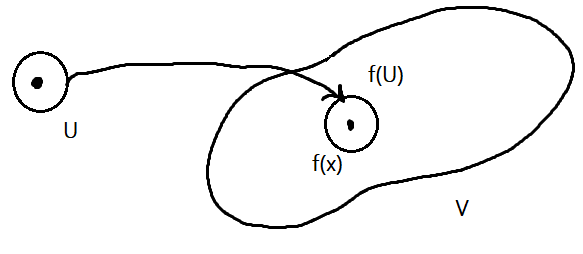
\includegraphics[width = 5cm]{lect4_3.png}
\end{wrapfigure}

\textbf{Определение.} X, Y --- топологические пространства, $f: \; X \to Y, \; x \in X.$ 

f \textbf{непрерывно} в x $\Leftrightarrow \; \forall$ окрестности $V \ni f(x) \; \exists$ окрестность $U \ni x$ т.ч. $f(U) \subset V.$ 

f \textbf{непрерывно} $\Leftrightarrow$ оно непрерывно в каждой $x \in X.$ 

\textbf{Предложение.} Пусть $f: X \to Y$ --- отображение топологических пространств, $x \in X, \; y = f(x).$ 

$\beta_{x}$ --- база топологии x, $\sigma_{y}$ --- предбаза окрестностей y. Тогда: 

f непрерывно в x $\Leftrightarrow \; \forall V \in \sigma_{y} \quad \exists$ окрестность $W \ni x$ т.ч. $f(w) \subset V, \; \exists V \in \beta_{x}$ т.ч. $U \subset W \Rightarrow f(x) \subset V.$ 

$(\Leftarrow)$ Пусть V --- окрестность y. $\exists V_{1}, ..., V_{p} \in \sigma_{y}$ т.ч. $V_{1} \cap ... \cap V_{p} \subset V; \; \forall i = 1, ..., p \; \exists U_{i} \in \beta_{x}$ т.ч. $f(V_{i}) \subset V_{i}, \; f(U_{1} \cap ... \cap U_{p}) \subset V.$

\textbf{Следствие.} $(X, \rho_{X}), \; (Y, \rho_{Y})$ --- метрические пространства, $x \in X.$ 

Отображение $f: X \to Y$ непрерывно в x $\Leftrightarrow \; \forall \varepsilon > 0 \; \exists \delta > 0$ т.ч. $\forall x' \in X,$ удовлетворяющей $\rho_{X}(x, x') < \delta,$ выполнено $\rho_{Y}(f(x), f(x')) < \varepsilon.$ 

\textbf{Доказательство.} Применить предложение к базам окрестностей x и f(x), состоящим из открытых шаров с центрами x и y. 

\textbf{Теорема.} X, Y --- топологические пространства, $f: X \to Y$ --- отображение. Следующие утверждения эквивалентны: 

(1) f непрерывно; 

$(2)!!! \; \forall$ открытых $V \subset Y \; f^{-1}(V)$ открыты в X --- часто берут в качестве определения непрерывности отображения;

(3) $\forall$ замкнутого $B \subset Y \quad f^{-1}(B)$ замкнуто в X; 

(4) $\forall A \subset X \; f(\overline{A}) \subset \overline{f(A)}.$

\textbf{Доказательство.} $(1) \Rightarrow (2).$ Пусть $V \subset Y$ --- открыто. $\forall x \in f^{-1}(V) \; \exists$ окрестность $U_{x} \ni x$ т.ч. $f(U_{x}) \subset V \Rightarrow U_{x} \subset f^{-1} \Rightarrow \bigcap_{x \in f^{-1}}
 U_{x} = f^{-1}(V) \Rightarrow f^{-1}(V)$ открыто. 
 
$(2) \Leftrightarrow (3)$ --- следствие из равенства $f^{-1}(Y \backslash B) = X \backslash f^{-1}(B) \; \forall B \subset Y.$ 
 
$(3) \Rightarrow (4) \; \forall A \subset X \; A \subset f^{-1}(f(A)) \subset f^{-1}(\overline{f(A)}),$ где $f^{-1}(\overline{f(A)})$ замкнуто, $\Rightarrow \overline{A} \subset f^{-1}(\overline{f(A)}),$ т.е. $f(\overline{A} \subset \overline{f(A)}.$ 

$(4) \Rightarrow (3).$ Пусть $B \subset Y$ замкнуто, $A = f^{-1}(B). \; f(\overline{A}) \subset \overline{f(A)} \subset \overline{B} = B \Rightarrow \overline{A} \subset g^{-1}(B) = A,$ т.е. $A$ замкнуто. 

$(2) \Rightarrow (1) \; \forall x \in X$ пусть $V$ --- окрестность $f(x) \Rightarrow VU = f^{-1}(V)$ --- окрестность $x,$ и $f(U) \subset V. \quad \square$ 

\textbf{Следствие.} Пусть $\tau_{1}, \; \tau_{2}$ --- топологии на множестве $X.$ Тогда $tau_{1} \subset \tau_{2} \Leftrightarrow$ отображение $f: (X, \tau_{2}) \to (X, \tau_{1}), \; f(x) = x$ --- непрерывно. Т.е. следует из второго пункта теоремы. 

\textbf{Предложение.} Пусть $f: X \to Y$ --- отображение топологических пространств, $\sigma$ --- предбаза $Y.$ $f$ непрерывно $\Leftrightarrow \; \forall V \in \sigma \; f^{-1}(V)$ открыто в $X.$ 

\textbf{Доказательство.} $(\Leftarrow)$ Пусть $V \subset Y$ открыто $\Rightarrow \; V = \underset{\alpha \in A}{\bigcup} \; \underset{\beta \in B_{\alpha}}{\bigcap} V_{\alpha \beta},$ где $V_{\alpha\beta} \in \sigma,$ а множества $B_{x}$ конечны. 
	
$\Rightarrow \; f^{-1}(V) = \underset{\alpha \in A}{\bigcup} \; \underset{\beta \in B_{\alpha}}{\bigcap} f^{-1}(V_{\alpha \beta})$ --- открыто в $X. \quad \square$ 

\textbf{Предложение.}$X, Y, Z$ --- топологические пространства, $F: X \to Y, \; g: Y \to Z, \; x \in X, \; y = f(x).$ 

Предположение: $f$ непрерывно в $x, \; g$ непрерывно в $y \; \Rightarrow g \circ f$ непрерывно в $x.$ В частности: если $f$ и $g$ непрерывно, то и $g \circ f$ непрерывно. 

\begin{figure}[htpb]
	\centering
	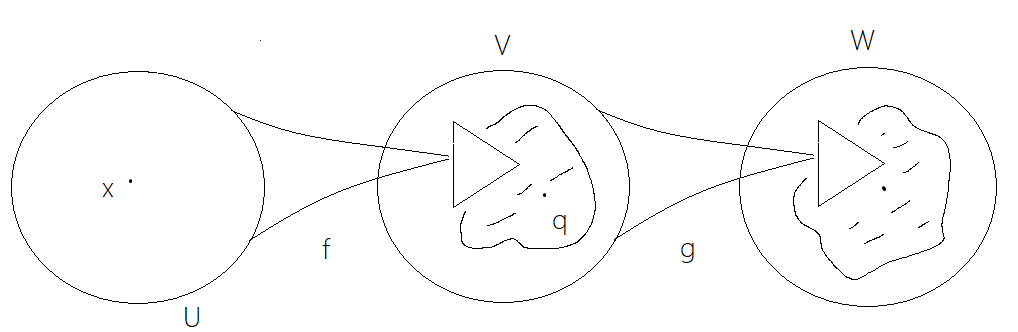
\includegraphics[width=0.8\linewidth]{lect5_1.png}
\end{figure}

\textbf{Доказательство.} Пусть $W$ --- окрестность $(g \circ f)(x) = g(x).$ 

Из того, что $\exists$ окрестность $V \ni y$ т.ч. $g(V) \subset W,$ и $\exists$ окрестность $U \ni x,$ т.ч. $f(U) \subset V,$ следует, что $(g \circ f)(U) \subset W.$ Картинка1 

\textbf{Определение.} $X, Y$ --- топологические пространства, $x \in X, \; f: X \to Y.$ 

$f$ \textbf{секвенциально непрерывно} в $x \; \Leftrightarrow \; \forall$ последовательности $(x_{n})$ в $X,$ т.ч. $x_{n} \to x,$ выполнено $f(x_{n}) \to f(x).$ 

\textbf{Предложение.} $f: X \to Y$ --- отображение топологических пространств, $x \in X.$ 

$(1) \; f$ непрерывна в $x \; \Rightarrow f$ секвенциально непрерывно в $x;$

$(2) \;$ Если $X$ удовлетворяет первой аксиоме счетности (например, метризуемо), то верно и обратное. 

\textbf{Доказательство.} (1) Пусть $x_{n} \to x, \; V$ --- окрестность $f(x).$ 

$\exists$ окрестность $U \ni x$ т.ч. $f(U) \subset V.$ $\exists N \in \mathbb{N}: \; \forall  n \geq N \; x_{n} \in U \; \Rightarrow \forall n \geq N \; f(x_{n}) \in V \; \Rightarrow f(x_{n}) \to f(x).$ 

(2) Предположение: $f$ не является непрерывным в $x.$ 

$\exists$ база окрестностей $\{U_{n}: \; n \in \mathbb{N}\}$ точки $x,$ т.ч. $U_{n} \supset U_{n + 1} \; \forall n;$ 

$\exists$ окрестность $V \ni f(x),$ т.ч. $f(U_{n}) \ni \subset V \; \forall n \in \mathbb{N}.$ 

Т.е. $\forall n \in \mathbb{N} \; \exists x_{n} U_{n},$ т.ч. $f(x_{n}) \ni V \Rightarrow x_{n} \to x,$ но $f(x_{n}) \ni \rightarrow f(x)$ --- противоречие. $\quad \square$ 

\textbf{Обозначение.} $C(X, Y) = \{f: X \to Y | \text{f непрерывно}\}.$ 

$C(X) = C(X, \mathbb{K}),$ где $\mathbb{K} = \mathbb{R}$ или $\mathbb{C}.$

\textbf{Определение.} $f \in C(X, Y)$ --- \textbf{гомеоморфизм} $\Leftrightarrow \exists g \in C(Y, X),$ т.ч. $fg = id_{Y}, \; gf = id_{X}.$ 

\textbf{Определение'} (эквивалентное предыдущему). $f: X \to Y$ --- \textbf{гомеоморфизм} $\Leftrightarrow \; f$ непрерывно и биективно, $f^{-1}$ непрерывно. 

\textbf{Наблюдение.} (1) $f: X \to Y$ --- гомеоморфизм $\Rightarrow f^{-1}: \; Y \to X$ --- гомеоморфизм. 

(2) $f: X \to Y, \; g: Y \to Z$ --- гомеоморфизм $\Rightarrow g \circ g: X \to Z$ --- гомеоморфизм. 

\textbf{Определение.} $X$ и $Y$ \textbf{гомеоморфны} $\Leftrightarrow \; \exists$ гомеоморфизм $X \to Y.$ 

\textbf{Определение.} $X, Y$ --- топологические пространства, $f: X \to Y.$ 

$f$ \textbf{открыто} $\Leftrightarrow \; \forall$ открытых $U \subset X \quad f(U)$ открыто в $Y.$ 

$f$ \textbf{замкнуто} $\Leftrightarrow \; \forall$ замкнутых $B \subset X \quad f(B)$ замкнуто в $Y.$ 

\textbf{Наблюдение.} Отображение $f: X \to Y$ --- гомеоморфизм $\Leftrightarrow f$ непрерывно, биективно и открыто или $\Leftrightarrow \; f: X \to Y$ непрерывно, биективно и замкнуто.

\textbf{Пример-упражнение 1.} $X$ --- нормированное пространство, $x \in X, \; r > 0.$ 

$f: B_{1}(0) \to B_{r}(x), \; f(y) = x + ry$ --- гомеоморфизм. 

\textbf{Пример-упражнение 2.} $X$ --- нормированное пространство. 

$ff: B_{1}(0) \to X, \; f(x) = \dfrac{x}{1 - ||x||}$ --- гомеоморфизм. 

\begin{wrapfigure}{R}{0.25\textwidth}
	\begin{tikzpicture}[scale=0.5]
	\draw (0,0) -- (8,0);
	\draw (0,0) -- (0,8) ;
	\draw (8,0) -- (8,8);
	\draw (0,8) -- (8,8);
	\draw [fill=white] (4,4) circle[radius=4];
	\draw (4,0) -- (4,8);
	\draw (0,4) -- (8,4);
	\end{tikzpicture}
\end{wrapfigure}

\textbf{Пример-упражнение 3.} $S^{1} = \{(x, y) \in \mathbb{R}^{2}: \; x^{2} + y^{2} = 1\}.$ 

$C = \{(x, y) \in \mathbb{R}^{2}: \max\{|x|, |y|\} = 1\}.$ 

$f: C \to S^{1}, \; f(p) = \dfrac{p}{||p||_{2}}$ --- гомеоморфизм. 

\begin{figure}[htpb]
	\centering
	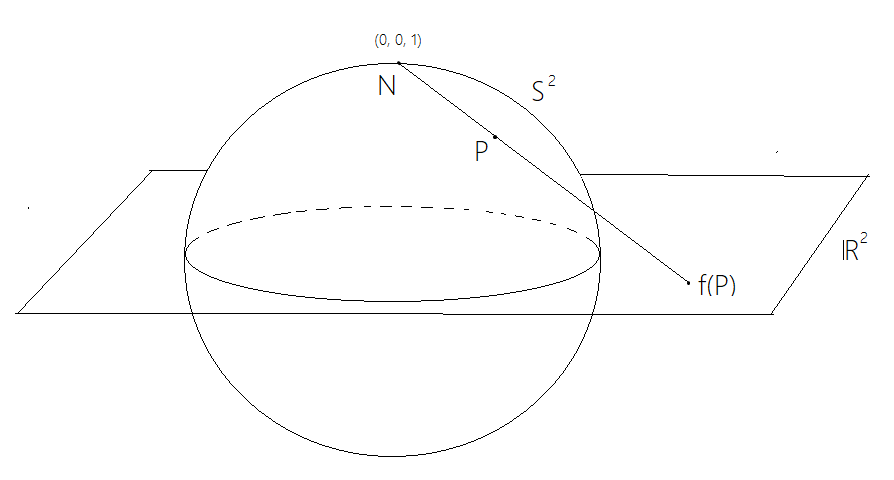
\includegraphics[width=0.8\linewidth]{lect5_3.png}
\end{figure}

\textbf{Пример-упражнение 4} (стереографическая проекция)

$S^{2} = \{(x, y, z) \in \mathbb{R}^{3}: \; x^{2} + y^{2} + z^{2} = 1\}$ --- сфера. 

$f: \; S^{2} \backslash \{\mathbb{N}\} \to \mathbb{R}^{2}$ --- гомеоморфизм. 

\textbf{Упражнение.} Построить аналогичный гомеоморфизм между $S^{n} \backslash \{\mathbb{N}\}$ и $\mathbb{R}^{n}.$ 

\textbf{Определение.} Топологическое пространство $M$ --- \textbf{топологическое многообразие ($C^{0}$-многообразие)} размерности $n,$ если 

(1) $M$ хаусдорфово; 

(2) $M$ со счетной базой; 

(3) $\forall x \in M \; \exists$ окрестность $U \ni x,$ гомеоморфная открытому подмножеству в $\mathbb{R}^{n}$ (здесь топология на $U$ определяется так: $V \subset U$ открыто в $U \; \Leftrightarrow V$ открыто в $M$). 

Если $U$ --- как в (3), $\varphi: \; U \to V$ --- гомеоморфизм, где $V \subset \mathbb{R}^{n}$ открыто, то $(U, \varphi)$ называется \textbf{картой} на $M.$ 

\textbf{Пример 1.} $\mathbb{R}^{n}$ --- топологическое многообразие. 

\textbf{Пример-упражнение 2.} Открытое подмножество в $\mathbb{R}^{n}$ --- топологическое многообразие (упражнение: доказать наличие счетной базы). 

\textbf{Пример-упражнение 3.} Сфера $S^{n} \subset \mathbb{R}^{n + 1}, \; S^{n} = \{x \in \mathbb{R}^{n + 1}: \; ||x||_{2} = 1\}$ --- топологическое многообразие. Упражнение: сколькими картами она покрывается? 

\subsection{Подпространства топологических пространств} 

$(x, \tau)$ --- топологическое пространство, $Y \subset X.$ 

\textbf{Обозначение.} $\tau_{Y} = \{V \cap Y: \; U \in \tau\}.$ 

\textbf{Наблюдение.} $\tau_{Y}$ --- топология на $Y.$ 

\textbf{Определение.} $\tau_{Y}$ --- топология, \textbf{индуцированная (унаследованная)} из $(x, \tau).$ $(Y, \tau_{Y})$ называется \textbf{топологическим подпространством} в $(X, \tau).$

\textbf{Предложение.} Пусть $(X, \rho)$ --- метрическое пространство, $Y \subset X, \; \tau_{\rho}$ --- топология на $Y,$ порожденная ограничением метрики $\rho$ на $Y \times Y \Rightarrow \tau_{\rho} = \tau_{Y}.$ 

\textbf{Доказательство.} Базу $\tau_{\rho}$ образуют шары $B_{r}^{Y} = \{z \in Y: \; \rho(z, y) < r\} \; (y \in Y, r > 0).$ 

\textbf{Замечание.} $B_{r}^{Y}(y) = B_{r}(y) \cap Y$ (где $B_{r}(y) = \{z \in X: \; \rho(z, y) < r\}) \Rightarrow B_{r}^{Y} \in \tau_{Y} \Rightarrow \tau_{\rho} \subset \tau_{Y}.$ 

Пусть $V \in \tau_{Y}; \; V = U \cap Y,$ где $U$ открыто в $X.$ 

Пусть $y \in V \Rightarrow \exists r > 0,$ т.ч. $B_{r}(y) \subset U \Rightarrow B_{r}^{Y}(y) \subset V \Rightarrow V \in \tau_{\rho} \Rightarrow \tau_{Y} = \tau_{\rho}. \quad \square$ 

\begin{figure}[htpb]
	\centering
	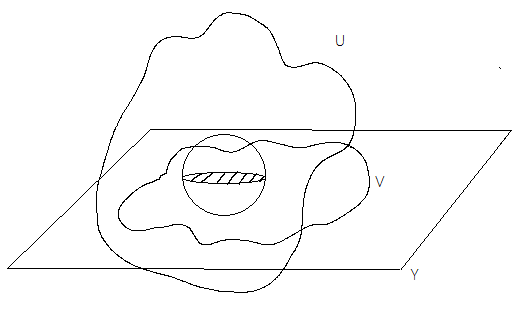
\includegraphics[width=0.6\linewidth]{lect5_4.png}
\end{figure}

\textbf{Обозначение.} $X$ --- множество, $Y \subset X.$ $y_{Y}: Y \to X, \; i_{Y}(y) = y \; \forall y \in Y$ --- \textbf{отображение включения} $Y$ в $X.$ 

\textbf{Теорема} (основные свойства индуцированной топологии)

$(X, \tau)$ --- топологическое пространство, $Y \subset X.$ Снабдим $Y$ индуцированной топологией $\tau_{y}.$ 

(1) $\tau_{Y}$ --- самая грубая топология на $Y,$ в которой $i_{Y}: \; Y \to X$ непрерывно;

(2) Если $Z$ --- топологическое пространство, то $f: Z \to Y$ непрерывно $\Leftrightarrow \; i_{Y} \circ f: Z \to X$ непрерывно. 

Иначе говоря, $f$ непрерывно как отображение из $Z$ в $Y \; \Leftrightarrow$ оно непрерывно как отображение из $Z$ в $X.$ 

\textbf{Доказательство.} (1) $i_{Y}^{-1}(U) = U \cap Y \Rightarrow i_{Y}$ непрерывно. Пусть $\sigma$ --- топология на $Y,$ т.ч. $i_{Y}: (Y, \sigma) \to X$ непрерывно $\Rightarrow \; \forall U \in \tau \; i_{Y}^{-1} (= U \cap Y) \in \sigma \Rightarrow \tau_{Y} \subset \sigma.$ 

(2) $\forall U \subset X \; (i_{Y} \circ f)^{-1}(U) = f^{-1}(i_{Y}(U)) = f^{-1}(U \cap Y).$

$i_{Y} \circ f$ непрерывно $\Leftrightarrow \forall U \in \tau \; (i_{Y} \circ f)^{-1}(U)$ открыто в $Z \Leftrightarrow \forall V \in \tau_{Y} \; f^{-1}(V)$ открыто в $Z$ и $\Leftrightarrow f$ непрерывна. $\square$

\textbf{Упражнение.} $\tau_{Y}$ --- единственная топология на $Y,$ удовлетворяющая (1), и единственная топология на $Y,$ удовлетворяющая (2).

[дальше лекция 21.11.19]

$(X, \tau)$ --- топологическое пространство $Y \subset X.$ 

$\tau_{Y} = \{U \cap Y: \; U \in \tau\}$ --- \textbf{индуцированная топология} на $Y.$ 

$i_{Y}: Y \to X$ --- отображение включения: $i_{Y}(y) = y \quad \forall y \in Y.$

$\tau_{Y}$ --- самая грубая топология на $Y,$ в которой $i_{Y}$ непрерывно. 

\textbf{Определение.} $f: X \to Y$ --- отображение множеств, $A \subset X.$ 

\textbf{Ограничение} $f$ на $A$ --- это $f|_{A}: \; A \to Y, (f|_{A})(a) = f(a) \quad \forall a \in A.$ 

\textbf{Предложение.} $X, Y$ --- топологические пространства, $A \subset X, \; f: X \to Y$ непрерывно $\Rightarrow f \backslash_{A}: A \to Y$ непрерывно. 

\textbf{Доказательство.} $f|_{A} = f \circ i_{A}. \quad \square$

\textbf{Предложение.} (1) Множество $B \subset Y$ замкнуто в $\tau_{Y} \; \Leftrightarrow B = F \cap Y$ для некоторого замкнутого $F \subset X.$ 

$\quad \quad \quad (2) \forall A \subset Y$ (замыкание $A$ в $(Y, \tau_{Y}) = \overline{A} \cap Y,$ где $\overline{A}$ --- замыкание $A$ в $X.$ 

\textbf{Доказательство.} (1) следует из формулы $Y \backslash B = (X \backslash B) \cap Y \; \forall B \subset Y.$ 

$\quad \quad \quad \quad \quad \quad \quad \quad \quad (2)$ (Замыкание $A$ в $Y$) = $\bigcap\{C \subset Y: \; C$ замкнуто в $(Y, \; \tau_{Y})$ и $C \supset A\} \overset{(1)}{=} \bigcap \{F \cap Y: \; F$ замкнуто в $X$ и $F \supset A\} = (\bigcap \{F: F$ замкнуто в $X$ и $F \supset A\}) \cap Y = \overline{A} \cap Y. \quad \square$ 

\textbf{Предложение.} $X$ --- топологическое пространство, $A \subset Y \subset X.$ 

(1) Если $Y$ открыто в $X,$ то $A$ открыто в $Y \; \Leftrightarrow A$ открыто в $X.$

(2) Если $Y$ замкнут в $X,$ то $A$ замкнут в $Y \; \Leftrightarrow A$ замкнут в $X.$

\textbf{Доказательство.} (1) $(\Rightarrow) \; A = Y \cap U,$ где $U$ открыто в $X \Rightarrow A$ открыто в $X.$

$\quad \quad \quad (\Leftarrow) \; A = Y \cap A,$ где $A$ открыто в $X, \; \Rightarrow A$ открыто в $Y.$ 

(2) Аналогично. $\quad \square$ 

\section{Инициальные топологии. Произведения топологических пространств}

\subsection{Инициальные точки} 

$X$ --- множество, $(X_{i}, \tau_{i})_{i \in I}$ --- семейство топологических пространств $(I \neq \varnothing); \; (f_{i}: X \to X_{i})_{i \in I}$ --- семейство отображений.

\textbf{Определение.} \textbf{Инициальная топология на $X,$} порожденная семейством $(f_{i})_{i \in I},$ --- это топология $\tau_{in}$ на $X$ с предбазой $\{f^{-1}_{i}(U): \; i \in I, U \in \tau_{i}\}.$ 

\textbf{Пример 1.} $X$ --- топологическое пространство, $Y \subset X.$

Инициальная топология на $Y$ = инициальная топология, порожденная $\{i_{Y}: \; Y \to X\}.$ 

\textbf{Обозначение.} $pt$ --- топологическое пространство,состоящее из одной точки.

\textbf{Пример 2.} $X$ --- множество. Инициальная топология на $X,$ порожденная $\{X \to pt\},$ --- антидискретная топология. 

\textbf{Теорема (основные свойства инициальной топологии).} $X$ --- множество, снабженное инициальной топологией, порожденной семейством $(f_{i}: \; X \to X_{i})_{i \in I}.$ 

(1) $\tau_{in}$ --- самая грубая топология на $X,$ в которой все $f_{i}$ непрерывны; 

(2) Если $Y$ --- топологическое пространство, то отображение $g\!: \; Y \to X$ непрерывно $\Leftrightarrow f_{i} \circ g\!: \; Y \to X_{i}$ непрерывно $\forall i.$ 

\begin{wrapfigure}{R}{0.2\textwidth}
		\begin{tikzpicture}[node distance=2cm, auto]
		\node (Y) {$Y$};
		\node(X) [right of=Y] {$X$};
		\node (X1) [below of=X] {$X_i$};
		\draw[->](Y) to node {$g$}(X);
		\draw[->](Y) to node [left] {$f_i\circ g$}(X1);
		\draw[->](X) to node [right=0.5ex] {$f_i$}(X1);
		\end{tikzpicture}
\end{wrapfigure}

\textbf{Доказательство.} (1) $\forall i \in I \; \forall U \in \tau_{i} \quad f_{i}^{-1}(U) \in \tau_{in} \; \Rightarrow f_{i}$ непрерывно.

Пусть $\sigma$ --- некоторая топология на $X,$ т.ч. $\forall i \in I \quad f_{i}: (X, \sigma) \to X_{i}$ непрерывно. 

$\forall i \in I \; \forall U \in \tau_{i} \quad f-{i}^{-1}(U) \in \sigma \; \Rightarrow$ (предбаза $\tau_{in}) \subset \sigma \Rightarrow \tau_{in} \subset \sigma.$ 

(2) $(\Rightarrow)$ Если $g$ непрерывно, то $f_{i} \circ g$ непрерывно, т.к. $f_{i}$ непрерывно. 

$(\Leftarrow)$ Пусть $f_{i} \circ g$ непрерывно $\forall i.$ 

Достаточно доказать: $\forall$ множества $V \subset X$ из предбазы $\tau_{in} \quad g^{-1}(V)$ открыто в $Y.$

$V = f_{i}^{-1}(U),$ где $U \subset X_{i}$ открыто $\Rightarrow g^{-1}(V) = g^{-1}(f_{i}^{-1}(U)) = (f_{i} \circ g)^{-1}(U)$ --- открыто в $Y. \quad \square$ 
 
\textbf{Упражнение.} $\tau_{in}$ --- единственная топология на $X$ со свойством (2).

\subsection{Произведения множеств} 

$(X_{i})_{i \in I}$ --- семейство множеств. 

\textbf{Определение.} \textbf{Произведение} семейства $(X_{i})_{i \in I}$ --- множество. 

$\underset{i \in I}{\text{П}} = \{x: \; I \to \underset{i \in I}{\bigcup} X_{i} \; | \; \forall i \in I \; x(i) \in X_{i}\}.$ 

\textbf{Частный случай.} Если $X_{i} = Y \quad \forall i,$ то $\underset{i \in I}{\text{П}} X_{i} = Y^{I}$ --- множество всех отображений $I \to Y.$

\textbf{Обозначения.} $\forall x \in \underset{i \in I}{\text{П}} X_{i}, \quad x_{i} = x(i), \quad x = (x_{i})_{i \in I} \; (x_{i} \in X_{i}).$ 

Если $I = \{1, 2, ..., n\},$ то вместо $\underset{i \in I}{\text{П}}X_{i}$ пишут $\overset{n}{\underset{i = 1}{\text{П}}}X_{i}$ или $X_{1} \times X_{2} \times ... \times X_{n}.$ 

В этом случае элементы $X_{1} \times ... \times X_{n}$ --- упорядоченные наборы $(x_{1}, ..., x_{n}),$ где $x_{i} \in X_{i}.$ 

\textbf{Обозначение.} $\forall j \in I \; p_{j}: \underset{i \in I}{\text{П}} X_{i} \to X_{j}, \; p_{j}(x) = x_{j}.$ 

$p_{j}$ --- \textbf{каноническая проекция} на $x_{j}.$ 

\subsection{Произведения топологических пространств} 

$(X_{i}, \tau_{i})_{i \in I}$ --- семейство топологических пространств, $X = \underset{i \in I}{\text{П}} X_{i}.$ 

\textbf{Определение.} \textbf{Топология произведения} (тихоновская топология) на $X$ --- это инициальная топология, порожденная семейством $\{p_{j}: X \to X_{j}\}_{j \in I}$ --- канонических проекций.
	
\textbf{Наблюдение.} (1) $\forall$ открытых $U \in X_{i}$ 

$(*) \; p_{i}^{-1}(U) = \underset{j \in J}{\text{П}} V_{j},$ где $V_{j} = 
\begin{cases}
U &\text{при j = i,}\\
X_{j} &\text{при $j \neq i.$}
\end{cases}$

Множества вида (*) образуют предбазу $X.$ 

(2) $\forall$ конечного $I_{0} \subset I, \; \forall i \in I_{0}$ пусть $U_{i} \subset X_{i}$ --- открытое множество. 

$(**)$ $\underset{i \in I_{0}}{\bigcap} p_{i}^{-1}(U_{i}) = \underset{j \in I}{V_{j}},$ где $V_{j} = 
\begin{cases}
U_{j}, &\text{если $j \in I_{0}$}\\
X_{j}, &\text{если $j \not \in I_{0}$}
\end{cases}$

Множества вида $(**)$ образуют базу $X.$ 

(3) Если $I$ конечно, то базу $X$ образуют множества вида $\underset{i \in I}{U_{i}},$ где $U_{i} \subset X_{i}$ открыто. 

\textbf{Предостережение-упражнение.} Если $I$ бесконечно, то $\underset{i \in I}{\text{П}}U_{i}$ необязательно открыто в $X$ (где $U_{i} \subset X_{i}$ открыто).

\textbf{Отступление.} Коммутативные диаграммы 

\begin{figure}[htpb]
	\begin{minipage}{.32\textwidth}
		\centering
		\begin{tikzpicture}[node distance=2cm, auto]
		\node (A) {$A$};
		\node(B) [right of=Y] {$B$};
		\node (C) [below of=X] {$C$};
		\draw[->](A) to node {$f$}(B);
		\draw[->](A) to node [left] {$g$}(C);
		\draw[->](B) to node [right=0.5ex] {$h$}(C);
		\end{tikzpicture}
		\captionof*{figure}{Коммутативна $\Leftrightarrow g = h \circ f$}
	\end{minipage}
	\begin{minipage}{.31\textwidth}
		\centering
		\begin{tikzpicture}[node distance=2cm, auto]
		\node (A) {$A$};
		\node(B) [right of=A] {$B$};
		\node (C) [below of=A] {$C$};
		\node (D) [below of=B] {$D$};
		\draw[->](A) to node {$f$}(B);
		\draw[->](A) to node [left] {$h$}(C);
		\draw[->](B) to node [right=0.5ex] {$k$}(D);
		\draw[->](C) to node {$g$}(D);
		\end{tikzpicture}
		\captionof*{figure}{Коммутативна $\Leftrightarrow k \circ f = g \circ h$}
	\end{minipage}
	\begin{minipage}{.31\textwidth}
		\centering
		\begin{tikzpicture}[node distance=2cm, auto]
		\node (A) {$A$};
		\node(B) [right of=A] {$B$};
		\node (C) [below of=A] {$C$};
		\node (D) [below of=B] {$D$};
		\draw[->](A) to node {$f$}(B);
		\draw[->](A) to node [left] {$h$}(C);
		\draw[->](B) to node [right=0.5ex] {$k$}(D);
		\draw[->](C) to node {$g$}(D);
		\end{tikzpicture}
		\captionof*{figure}{Коммутативна $\Leftrightarrow f = k \circ g \circ h$}
	\end{minipage}
\end{figure}

\textbf{Теорема (универсальное свойство произведения).} $(x_{i})_{i \in I}$ --- семейство топологических пространств, $X = \underset{i \in i}{\text{П}} X_{i}, \quad p_{i}: X \to X_{i}$ --- каноническая проекция, $Y$ --- топологическое пространство. 

\begin{wrapfigure}{L}{0.3\textwidth}
	\begin{tikzpicture}[node distance=2cm, auto]
	\node (Y) {$Y$};
	\node(X) [right of=Y] {$X$};
	\node (X1) [below of=X] {$X_i$};
	\draw[->](Y) to node {$f$}(X);
	\draw[->](Y) to node [left] {$f_i$}(X1);
	\draw[->](X) to node [right=0.5ex] {$p_i \quad \quad (D)$}(X1);
	\end{tikzpicture}
\end{wrapfigure}

Тогда $\forall$ семейства $(f_{i}: Y \to X_{i})_{i \in I}$ непрерывных отображений $\exists !$ непрерывное отображение $f: Y \to X,$ т.ч. диаграмма $(D)$ коммутативна $\forall i \in I.$ 

\textbf{Доказательство.} Определим $f: Y \to X$ так: $(f(y))_{i} = f_{i}(y) \quad \forall y \in Y, \; \forall i \in I.$

Отображение $f$ делает диаграмму $(D)$ коммутативной и является единственным отображением с этим свойством. Его непрерывность следует из теоремы о свойствах инициальной топологии. $\square$ 

\textbf{Предложение.} $(x_{i}, \; \rho_{i}) \; (i = 1, 2, 3, ..., n)$ --- метрическое пространство, $X = \underset{i = 1}{\text{П}} X_{i}.$

Определим $\rho\!\!: X \times X \to [0; +\infty)$ так: $\rho(x, y) = \underset{1 \leq i \leq n}{\max} \rho_{i}(x_{i}, y_{i}).$ 

Тогда $\rho$ --- метрика на $X,$ и она порождает топологию произведения на $X.$ 

\textbf{Доказательство.} Упражнение. $\rho$ --- метрика. Обозначим $\tau$ = топология на $X,$ $\tau_{\rho}$ --- топология, порожденная $\rho.$ 

\textbf{Заметим:} $\rho(x, y) < r \Leftrightarrow \rho_{i}(x_{i}, y_{i}) < r \quad \forall i = 1, ..., n \quad \Leftrightarrow B_{r}(x) = \overset{n = 1}{\underset{i = 1}{\text{П}}} B_{r}(x_{i}) \Rightarrow B_{r}(x)$ открыт в $\tau \Rightarrow \tau_{\rho} \subset \tau.$

Пусть $U$ --- множество из базы $\tau; \; U = \overset{n}{\underset{i = 1}{\text{П}}} U_{i},$ где $U_{i} \subset X_{i} \; \forall i$ открыто. 

Пусть $x \in U.$ Тогда $\forall i = 1, ..., n \quad x_{i} \in U_{i} \Rightarrow \exists r_{i} > 0$ т.ч. $B_{r_{i}} (x_{i}) \subset \overset{n}{\underset{i = 1}{\text{П}}} U_{i} = U.$ 

$\Rightarrow U$ открыто в $\tau_{\rho} \Rightarrow \tau \subset \tau_{\rho} \Rightarrow \tau = \tau_{\rho}. \quad \square$ 

\textbf{Следствие.} $\mathbb{K} = \mathbb{R}$ или $\mathbb{C}.$ Стандартная топология на $\mathbb{R}^{n},$ порожденная $|| \cdot ||_{\infty}$ (или $|| \cdot ||_{1}, \; || \cdot ||_{2}),$ совпадает с топологией произведения $\mathbb{K} \times ... \times \mathbb{K}.$ 
 
\textbf{Доказательство.} Определим $f\!\!: Y \to X$ так: $(f(y))_{i} = f_{i}(y) \quad \forall y \in Y \quad \forall i \in I.$ 

Отображение $f$ делает диаграмму (D) коммутативной и является отображением с этим свойством. Его непрерывность следует из теоремы о свойствах инициальной топологии. $\square$

\textbf{Определение.} $(X_{i}, \rho_{i}) \; (i = 1, ..., n)$ --- метрические пространства, $X = \underset{i = 1}{\overset{n}{\text{П}}} X_{i}.$ 

Определим $\rho\!\!: \; X \times X \to [0; +\infty]$ так: $\rho(x, y) = \underset{1 \leq i \leq n}{\max} \rho_{i} (x_{i}, y_{i}).$ 

Тогда $\rho$ --- метрика на $X,$ и она порождает топологию произведения на $X.$ 

\textbf{Доказательство.} Упражнение. $\rho$ --- метрика. 

Обозначение. $\tau$ = топология произведения на $X, \; \tau_{\rho}$ --- топология, порожденная $\rho.$ Заметим: $\rho(x, y) < r \Rightarrow \rho_{i} (x_{i}, y_{i}) < r \quad \forall i = 1, ..., n \Rightarrow B_{r} (x) = \underset{i = 1}{\overset{n}{\text{П}}} B_{r}(X_{i}) \Rightarrow B_{r} (X)$ открыто в $\tau \; \Rightarrow \tau_{\rho} \subset \tau.$ 

Пусть $U$ --- множество из базы $\tau; \; U = \underset{i = 1}{\overset{n}{\text{П}}} U_{i},$ где $U_{i} \subset X_{i} \quad \forall i$ открыто. 

Пусть $x \in U.$ Тогда $\forall i = 1, ..., b \quad x_{i} \in U_{i} \Rightarrow \exists r_{i} > 0: \; B_{r}(x_{i}) \subset U_{i}.$ 

Обозначим $r = \underset{1 \leq i \leq n}{\min} r_{i} \Rightarrow B_{r}(x) = \underset{i = 1}{\overset{n}{\text{П}}} B_{r} (x_{i}) \subset \underset{i = 1}{\overset{n}{\text{П}}} B_{r_{i}} (x_{i}) \subset \underset{i = 1}{\overset{n}{\text{П}}} U_{i} = U \Rightarrow U$ открыто в $\tau_{\rho} \Rightarrow \tau \subset \tau_{\rho} \Rightarrow \tau = \tau_{\rho}. \quad \square$ 

\textbf{Следствия.} Стандартная топология на $\mathbb{K}^{n},$ порожденная $|| \cdot ||_{\infty}$ (или $|| \cdot||_{1}, \; || \cdot ||_{2}),$ где $\mathbb{K} = \mathbb{R}$ или $\mathbb{C},$ совпадает с топологией произведения $\mathbb{K} \times ... \times \mathbb{K}.$ 

$X$ --- множество, $(X_{i})_{i \in I}$ --- топологические пространства, $(f_{i}: X \to X_{i})_{i \in I}.$ 

$\{f_{i}^{-1}(U)\!: U \subset X_{i}$ открыто, $i \in I$\} является предбазой инициальной топологии $\tau_{in},$ порожденной $(f_{i}).$ 

$(X_{i})_{i \in I}, \; (Y_{i})_{i \in I}$ --- семейства множеств, $f_{i}: \; (X_{i} \to Y_{i})_{i \in I}$ --- семейство отображений. 

\textbf{Определение.} Декартово произведение семейства $(f_{i})$ --- отображение $\underset{i \in I}{\text{П}} f_{i}: \; \underset{i \in I}{\text{П}} X_{i} \to \underset{i \in I}{\text{П}} Y_{i}. \quad (X_{i})_{i \in I} \to (f_{i}(X_{i}))_{i \in I}.$

\textbf{Предположение.} Пусть $(X_{i})_{i \in I}, (Y_{i})_{i \in I}$ --- семейства топологических пространств, $f_{i}: X_{i} \to Y_{i})_{i \in I}$ --- семейство непрерывных отображений $\Rightarrow \text{П} f_{i}: \text{П} X_{i} \to \text{П} Y_{i}$ непрерывно. 

\textbf{Доказательство.} П$X_{i} = X, \; \text{П}Y_{i} = Y \; \text{П} f_{i} = f.$

\begin{wrapfigure}{R}{0.2\textwidth}
	\begin{tikzpicture}[node distance=2cm, auto]
	\node (X) {$X$};
	\node(Y) [right of=X] {$Y$};
	\node (X1) [below of=X] {$X_i$};
	\node (Y1) [below of=Y] {$Y_i$};
	\draw[->](X) to node {$f$}(Y);
	\draw[->](X) to node [left] {$p^X_i$}(X1);
	\draw[->](X1) to node [below] {$p_i$}(Y1);
	\draw[->](Y) to node [right=0.5ex] {$p^Y_i$}(Y1);
	\end{tikzpicture}
\end{wrapfigure}

$f$ непрерывно $\Leftrightarrow \; p_{i}^{Y} \circ f$ непрерывно $\forall i$ (см. свойства инициальной топологии) $\Leftrightarrow f_{i} \circ p_{i}^{X}$ непрерывно, а это верно по условию. $\square$ 

\textbf{Следствие.} $X$ --- топологическое пространство. $\mathbb{K} = \mathbb{R}$ или $\mathbb{C}, \; C(X) = C(X, \mathbb{R}).$

Тогда $\forall f, \; g \in C(X) \; f + g \in C(X)$ и $fg \in C(X).$ Если $f(x) \neq 0 \quad \forall x \in X \Rightarrow \dfrac{1}{f} \in C(X).$ 

$X \underset{x \underset{\text{непрерывно}}{\mapsto} (x, x)}{\overset{\Delta}{-\!\!\!-\!\!\!-\!\!\!-\!\!\!-\!\!\!\to}}X \times X \underset{\text{непрерывно}}{\overset{f \times g}{-\!\!\!-\!\!\!-\!\!\!-\!\!\!-\!\!\!\to}} \mathbb{K} \times \mathbb{K} \underset{\text{непрерывно}}{\overset{+}{-\!\!\!-\!\!\!-\!\!\!-\!\!\!-\!\!\!\to}} \mathbb{K},$ т.е. $X \overset{f + g}{-\!\!\!-\!\!\!-\!\!\!-\!\!\!-\!\!\!\to} \mathbb{K}, \; \Rightarrow f + g$ непрерывно. Аналогично $fg$ непрерывно. 

$X \underset{\text{непрерывно}}{\overset{f}{-\!\!\!-\!\!\!-\!\!\!-\!\!\!-\!\!\!\to}} \mathbb{K} \backslash \{0\} \underset{\text{непрерывно}}{\overset{t \mapsto \dfrac{1}{t}}{-\!\!\!-\!\!\!-\!\!\!-\!\!\!-\!\!\!\to}},$ т.е. $X \overset{\dfrac{1}{t}}{\to} \mathbb{K} \Rightarrow \dfrac{1}{f}$ непрерывно. $\square$ 

\textbf{Предложение.} Топологическое пространство $X$ хаусдорфово $\Leftrightarrow$ диагональ $D_{x} = \{(x, \; x): \; x \in X\} \subset X \times X$ замкнута в $X \times X.$ 

\begin{wrapfigure}{R}{0.3\textwidth}
	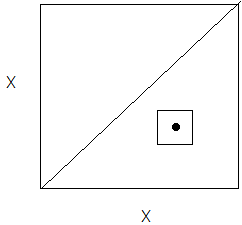
\includegraphics[width = 5cm]{lect7_2.png}
\end{wrapfigure}

\textbf{Доказательство.} $D_{X}$ замкнута в $X \times X \; \Leftrightarrow \forall p \in (X \times X) \backslash D_{X} \; \exists$ окрестность $W \ni p$ вида $W = U \times V,$ где $U, V$ --- открыто в $X,$ т.ч. $W \cap D_{x} = \varnothing.$ 

$\Leftrightarrow \forall x, y \in X,$ т.ч. $x \neq y \; \exists$ открытые $U, V \subset X,$ т.ч. $x \in U, y \in V$ и $U \cap V = \varnothing \Leftrightarrow X$ --- хаусдорфово. $\square$ 

\textbf{Следствие 1. Предложение.} $X, Y$ --- топологические пространства, $Y$ --- хаусдорфово, $f, g: X \to Y$ непрерывно $\Rightarrow \; \{x \in X: \; f(x) = g(x)\}$ замкнуто в $X.$

\textbf{Доказательство.} $F: \; X \to Y \times Y, \; F(x) = (f(x), g(x))  \; F$ непрерывно, $\{x: \; f(x) = g(x)\} = F^{-1}(D_{Y}),$ а $D_{Y}$ замкнуто в $Y \times Y. \quad \square$

\textbf{Следствие 2.} $X, \; Y$ --- топологические пространства, $Y$ --- хаусдорфово, $f, g: X \to Y$ непрерывно. Пусть $X_{0} \subset X$ --- плотное подмножество, т.е. замыкание содержит все пространство, $f/_{X_{0}} = g/_{X_{0}} \Rightarrow f = g.$ 

\textbf{Доказательство.} Множество $S = \{x \in X: f(x) = g(x)\}$ замкнуто и содержит $X_{0} \; \Rightarrow S = X. \quad \square$

\section{Финальные топологии и дизъюнктные объединения}

\subsection{Финальные топологии}

$X$ --- множество, $(X_{i}, \tau_{i})_{i \in I}$ --- семейство топологических пространств. $(f_{i}: X_{i} \to X)_{i \in I}$ --- семейство отображений.

\textbf{Определение.} \textbf{Финальная топология} на $X,$ порожденная $(f_{i})_{i \in I}$ --- это $\tau_{f_{i \not \in I}} = \{U \subset X: f_{i}^{-1}(U) \in \tau_{i} \quad \forall i \in I\}.$

\textbf{Замечание.} $\tau_{f_{in}}$ является топологией на $X.$

\textbf{Предложение.} Финальная топология на $X,$ порожденная отображением $\{\varnothing \to X\},$ --- дискретная топология. 

\textbf{Теорема 1 (основные свойства финальной топологии)}

(1) $\tau_{f_{in}}$ --- самая тонкая топология на $X,$ т.ч. все $f_{i}: \; X_{i} \to X$ непрерывны. 

(2) Если $Y$ --- топологическое пространство, то отображение $g: \; X \to Y$ непрерывно $\Leftrightarrow \; g \circ f_{i}$ непрерывно $\forall i.$ 

\begin{wrapfigure}{R}{0.2\textwidth}
	\begin{tikzpicture}[node distance=2cm, auto]
	\node (X) {$X$};
	\node(Y) [right of=X] {$Y$};
	\node (X1) [below of=X] {$X_i$};
	\draw[->](X1) to node {$f_i$}(X);
	\draw[->](X) to node {$g$}(Y);
	\draw[->](X1) to node [right=0.5ex] {$g\circ f_i$}(Y);
	\end{tikzpicture}
\end{wrapfigure}
	
\textbf{Доказательство.} (1) $\forall i \in I \quad \forall \; U \subset \tau_{f_{in}} \quad f_{i}^{-1} \in \tau_{i}$ --- верно по определению $\tau_{f_{in}} \Rightarrow f_{i}^{-1}$(открытое) = открытое $\Rightarrow f_{i}$ непрерывно. 

Пусть $\sigma$ --- топология на $X,$ т.ч. $\forall i \in I \quad f_{i}: X_{i} \to (X, \sigma)$ непрерывно $\forall \; U \in \sigma \quad \forall i \in I \quad f^{-1}_{i}(U) \in \tau_{i} \Rightarrow U \in \tau_{fin} \Rightarrow \sigma \subset \tau_{fin}.$ 

(2) $g$ непрерывно $\Leftrightarrow \forall \; V \subset Y$ открыто, $g^{-1}(V) \in \tau_{fin} \Leftrightarrow \forall$ открытого $V \subset Y \quad \forall i \in I \quad f_{i}^{-1}(g^{-1}(V)) = (g \circ f_{i})^{-1}(V) \in \tau_{i}.$ 

\textbf{Упражнение.} $\tau_{fin}$ --- топология на $X,$ обладающая свойством (2).

\subsection{Дизъюнктное объединение множеств}

$(X_{i})_{i \in I}$ --- семейство множеств. 

\textbf{Определение.} \textbf{Дизъюнктное объединение} семейства $(X_{i})_{i \in I}$ --- множество $\underset{i \in I}{\sqcup} X_{i} = \{(x, i): i \in I, x \in X_{i}\}.$ 

\textbf{Обозначение}. $\forall j \in I \quad q_{j}: X_{j} \to \underset{i \in I}{\sqcup} X_{i}, \; q_{j}(X) = (X, j)$ --- каноническое вложение $X_{j}$ в $\underset{i \in I}{\sqcup} X_{i}.$ 

\textbf{Наблюдение.} (1) $q_{j}$ --- инъекция $\forall j;$ 

(2) $q_{i} (X_{i}) \cap q_{j}(X_{j}) = 0 \quad \forall i \neq j;$

(3) $\underset{i \in I}{\sqcup} X_{i} = \underset{i \in I}{q_{i}} (X_{i}).$

\textbf{Соглашение.} Отождествляем $X_{j}$ c $q_{j}(X)$ посредством $q_{j}.$

\subsection{Дизъюнктное объединение топологических пространств (несвязные суммы)}

$(X_{i})_{i \in I}$ --- семейство топологических пространств, $X = \underset{i \in I}{\sqcup} X_{i}, \; q_{j}\!\!: X_{j} \to X.$

\textbf{Определение.} \textbf{Топология дизъюнктного объединения} на $X$ --- финальная топология, порожденная семейством $(q_{i}\!\!: X_{i} \to X)_{i \in I}$ канонических вложений.

Таким образом, $U \subset X$ открыто $\Leftrightarrow U \cap X_{i}$ открыто в $X_{i} \quad \forall i \in I.$ 

\textbf{Теорема 2 (универсальное свойство дизъюнктных объединений)}

$(x_{i})_{i \in I}$ --- семейство топологических пространств, $Y$ --- топологическое пространство, $X = \underset{i \in I}{\sqcup} X_{i}.$ 

Тогда $\forall$ семейства непрерывных отображений $(f_{i}: X_{i} \to Y)_{i \in I} \; \exists !$ непрерывное $f: X \to Y,$ т.ч. диаграмма $(D)$ коммутативна $\forall i \in I.$ 

\begin{wrapfigure}{L}{0.3\textwidth}
	\begin{tikzpicture}[node distance=2cm, auto]
	\node (X) {$X$};
	\node(Y) [right of=X] {$Y$};
	\node (X1) [below of=X] {$X_i$};
	\draw[->](X1) to node {$q_i$}(X);
	\draw[->](X) to node {$f$}(Y);
	\draw[->](X1) to node [right=0.5ex] {$f_i \quad \quad (D)$}(Y);
	\end{tikzpicture}
\end{wrapfigure}

\textbf{Доказательство.} Зададим $f: X \to Y$ так: $f((x, i)) = f_{i}(x) \quad (\forall i \in I, \forall x \in X_{i}). \quad (*)$

Отображение $f$ делает $(D)$ коммутативной и является единственным отображеним с этим свойством (т.к. (*) эквивалетно $f(q_{i}(x)) = f_{i}(x)$). Непрерывность $f$ --- из теоремы 1. $\square$ 

\section{Связные топологические пространства} 

\textbf{Определение.} Топологическое пространство $X$ \textbf{связно} $\Leftrightarrow \; X$ непредставимо в виде $X = U \cup V,$ где $U, V \subset X$ открыто, непусто, $U \cap V = \varnothing.$ Иначе $X$ называется \textbf{несвязным.}

\begin{wrapfigure}{R}{0.2\textwidth}
	\begin{tikzpicture}[node distance=2cm, auto]
	\node (X) {$X$};
	\node(Y) [right of=X] {$Y$};
	\node (X1) [below of=X] {$X_i$};
	\draw[->](X1) to node {$(D)$}(X);
	\draw[->](X) to node {}(Y);
	\draw[->](X1) to node {}(Y);
	\end{tikzpicture}
\end{wrapfigure}

Подмножество $Y \subset X$ называется \textbf{связным} $\Leftrightarrow$ оно связано как топологическое пространство в индуцированной топологии.

\textbf{Наблюдение.} $X$ связно $\Leftrightarrow X$ непредставимо в виде $X = A \cup B,$ где $A, B$ замкнуты, непусты, $A \cap B = \varnothing \; \Leftrightarrow \cancel{\exists}$ подмножества $A \subset X, \; A \neq X, A \neq \varnothing,$ открыто и замкнуто одновременно. 

\textbf{Пример.} Дискретное пространство, состоящее более чем из 1 точки, несвязно. 

\textbf{Пример.} Антидискретное пространство связно. 

\textbf{Пример.} $\mathbb{R} \backslash \{0\}$ несвязно, т.к. $\mathbb{R} \backslash \{0\} = (-\infty, 0) \cup (0, +\infty).$ 

\usetikzlibrary{patterns}
\begin{wrapfigure}{R}{0.3\textwidth}
	\begin{tikzpicture}
	\draw[->](-1, 0) -- (3, 0);
	\draw[->](0, -2) -- (0, 2);
	\draw [pattern=north west lines] (0,0) circle[radius=8pt];
	\draw [pattern=north west lines] (2,0) circle[radius=8pt];
	%\draw [ultra thick] (0,0) -- (2,2);
	%\draw [help lines] (1,0) -- (1,1) -- (0,1);
	\end{tikzpicture}
\end{wrapfigure}

\textbf{Пример.} $\overline{B_{1}}(0, 0) \cup \overline{B_{1}}(0, 3) \subset \mathbb{R}^{2}$ --- несвязное.

\textbf{Пример.} $X, Y$ --- непустые топологические пространства $\Rightarrow X \sqcup Y$ несвязно (т.к. X, Y открыты в $X \sqcup Y).$

\textbf{Пример.} $\forall A \subset \mathbb{Q}$ (с топологией, индуцированной из $\mathbb{R}),$ состоящего более чем из одной точки, несвязно.

$a, \; b \in A, \; a  < b \quad \exists$ иррациональное $c \in \mathbb{R}: \; a < c < b.$ 

$\bigcup = A \cap (-\infty, c), \quad V = A \cap (c, +\infty) \Rightarrow U, V$ открыто в $A, \; U \cap V = \varnothing$ и $U \cup V = A.$

\textbf{Предложение.} Отрезок $[a, b] \subset \mathbb{R}$ связен.

\textbf{Доказательство.} Предположим, $[a, b] = U \cup V, \quad U, V \subset [a, b]$ открыты в топологии отрезка $[a, b]),$ непусты, $U \cap V = \varnothing.$

Можем считать: $b \in V \Rightarrow \exists \varepsilon > 0,$ т.ч. $(b - \varepsilon, b] \subset V. \quad (1)$ 

Обозначим $c = \sup U.$ Заметим: $c > a$ (иначе бы $U = \{a\}$ --- противоречие), $c < b$ в силу (1). 

Если $c \in U \Rightarrow \exists \delta > 0,$ т.ч. $(c - \delta, c + \delta) \subset U \Rightarrow c + \dfrac{\delta}{2} \in U$ --- противоречие с определением $c.$

Если $c \in V \Rightarrow \exists \delta > 0,$ т.ч. $(c - \delta, c + \delta) \subset V \Rightarrow \forall x \in U \quad x \leq c - \delta$ --- противоречие с определением $c \Rightarrow c \not \in U \cup V = [a, b]$ --- противоречие $\Rightarrow [a, b]$ связен. $\square$ 

\subsection{Свойства связных пространств}

\textbf{Теорема (свойства связных пространств)}

(1) $X, \; Y$ --- топологические пространства, $X$ связно, $f\!\!: X \to Y$ непрерывно $\Rightarrow f(X)$ связно. 

(2) Пусть $X = U \cup V, \; U, \; V$ открыто, $U \cap v = \varnothing;$ пусть $A \subset X$ связно $\Rightarrow A \subset U$ либо $A \subset V.$ 

(3) $A, B \subset X, \; A \subset B \subset \overline{A},$ $A$ связно $\Rightarrow B$ связно.

(4) Пусть $(A_{i})_{i \in I}$ --- семейство связных подмножеств $X,$ имеющих общую точку $\Rightarrow \underset{i \in I}{A_{i}}$ связно.

(5) Пусть любые $x, y \in X$ лежат в некотором связном подмножестве $X \Rightarrow X$ связно. 

(6) $X_{1}, ..., X_{n}$ --- связные топологические пространства $\Rightarrow X_{1} \times ... \times X_{n}$ связно.

\textbf{Доказательство.} (1) Можем считать: $f(X) = Y.$ Пусть $Y = U \cup V, \; U, V \subset Y$ открыты, непусты, $U \cap V = \varnothing.$ 

$f$ --- сюръекция $\Rightarrow X = f^{-1}(U) \cup f^{-1}(V),$ где $f^{-1}(U), \;  f^{-1}(V)$ открыты, непусты, не пересекаются, --- противоречие. 

(2) $A = (U \cap A) \cup (V \cap A) \Rightarrow U \cap A$ либо $V \cap A$ пусто. Если $U \cap A = \varnothing \Rightarrow A = V \cap A,$ т.е. $A \subset V,$ где $U \cap A, \; V \cap A$ открыты в $A$ и не пересекаются. 

(3) Можем считать: $B = X,$ тогда $\overline{A} = X.$ Пусть $X = U \cup V, \; U, V \subset X$ открыты, непусты, $U \cap V = \varnothing.$

Из (2): $A \subset U$ либо $A \subset V.$ Пусть $A \subset U \Rightarrow A \cap V = \varnothing$ --- противоречие с тем, что $\overline{A} = X \Rightarrow X$ связно.

(4) Можем считать: $\underset{i \in I}{\bigcup} A_{i} = X.$ Пусть $a \in A_{i} \quad \forall i \in I.$ 

Пусть $X = U \cap V, \quad U, V \subset X$ открыты, непусты, $U \cap V = \varnothing.$ 

Пусть $a \in U.$ Из (2): $A_{i} \subset U \quad \forall i \in I \Rightarrow V = \varnothing$ --- противоречие $\Rightarrow X$ связно.

(5) Зафиксируем $\forall x \in X.$ 

$\forall y \in X \quad \exists$ связное $A_{xy} \subset X,$ т.ч. $x, y \in A_{xy} \Rightarrow \underset{y \in X}{\bigcup} A_{xy} = X.$ Из (4) $X$ связно.

(6) Достаточно доказать для $n = 2$ (индукция). Обозначим $X_{1} = X, X_{2} = Y.$ Зафиксируем $p = (x_{1}, y_{1}) \in X \times Y, \; q = (x_{2}, y_{2}) \in X \times Y.$ 

\begin{wrapfigure}{R}{0.2\textwidth}
	\begin{tikzpicture}[scale=0.5]
	\draw (0,0) --  node[below] {$X$} (7,0);
	\draw (0,0) -- node[left] {$Y$} (0,5) ;
	\draw (7,0) -- (7,5);
	\draw (0,5) -- (7,5);
	\draw (1, 0) -- (1, 5);
	\draw (0, 4) -- (7, 4);
	\draw [fill=black] (1,1) circle[radius=2pt] node[right] {$p$};
	\draw [fill=black] (5, 4) circle[radius=2pt] node[below] {$q$};
	\draw [fill=black] (1, 4) circle[radius=2pt];
	\end{tikzpicture}
\end{wrapfigure}

Обозначим $A = \{x_{1}\} \times Y, \; B = X \times \{y_{2}\}.$ $A$ гомеоморфно $Y, \; B$ гомеоморфно $X \Rightarrow A, B$ связно. 

$(x_{1}, y_{2}) \in A \cap B \Rightarrow A \cap B = \varnothing \underset{(4)}{-\!\!-\!\!\!\to} A \cup B$ связно. 

$p, q \in A \cup B \underset{5}{\Rightarrow} X \to Y$ связно. $\square$ 

\textbf{Упражнение.} Доказать: произведение $\forall$ семейства топологических пространств связно. 

\textbf{Определение.} $X$ --- топологическое пространство, $x, y \in X.$ Пусть в $X$ из $x$ в $y$ --- непрерывное отображение $f\!: \; [0, 1] \to X,$ т.ч. $f(0) = x, f(1) = y.$

\begin{wrapfigure}{R}{0.4\textwidth}
	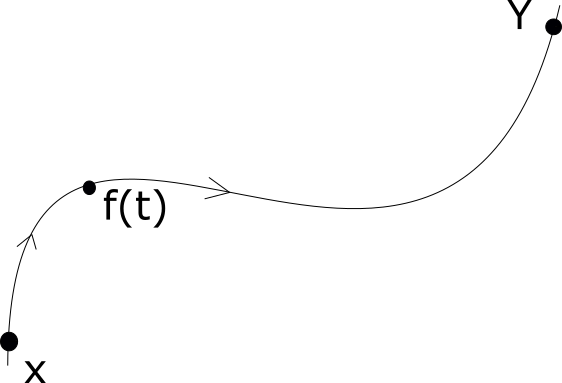
\includegraphics[width=0.8\linewidth]{lect8_3.png}
\end{wrapfigure}

\subsection{Линейно связные пространства}

\textbf{Определение.} $X$ \textbf{линейно связно,} если $\forall x, y \in X \quad \exists$ путь из $x$ в $y.$ 

\textbf{Предложение.} $X$ линейно связно $\Rightarrow X$ связно.

\textbf{Доказательство.} Пусть $x, y \in X, \; f: [0, 1] \to X$ --- пусть из $x$ в $y, \; C = f([0, 1]).$

$C$ связно (т.к. [0, 1] связен, см. пункт (1) теоремы), $x, y \in C.$ Теорема, п. (5) $\Rightarrow X$ связно. $\square$ 

\subsection{Свойства линейно связных пространств}

\textbf{Теорема (свойства линейно связных пространств)}

(1) $X, \; Y$ --- топологические пространства, $X$ линейно связно, $f\!\!: X \to Y$ непрерывно $\Rightarrow f(X)$ линейно связно;

(2) $(A_{i})_{i \in I}$ --- семейство линейно связных подмножеств в $X,$ имеющих общую точку $\Rightarrow \underset{i \in I}{\bigcup} A_{i}$ линейно связно; 

(3) $X_{1}, ..., X_{n}$ линейно связны $\Rightarrow X_{1} \times ... \times X_{n}$ линейно связны. 

\begin{wrapfigure}{R}{0.4\textwidth}
	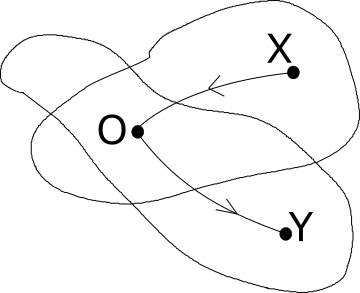
\includegraphics[width=0.8\linewidth]{lect8_4.png}
	\\ \; \\
	\begin{tikzpicture}[scale=1]
	\draw node[below] {$x$} (2,0) -- (5,0) node[below] {$y$};
	\draw[->] (0,0) -- (2,0);
	\draw [fill=black] (0, 0) circle[radius=2pt];
	\draw [fill=black] (5, 0) circle[radius=2pt];
	\end{tikzpicture}
\end{wrapfigure}

\textbf{Доказательство.} Упражнение. Подсказка к (2) --- рисунок.

\textbf{Пример 1.} $X$ --- нормированное пространство над $\mathbb{R} \Rightarrow X$ линейно связно. 

Действительно: $\forall x, y \in X$ рассмотрим $f: [0, 1] \to X, \; f(t) = ty + (1 - t)x.$ $f$ непрерывно (упражнение), $f(0) = x, \; f(1) = y.$

\textbf{Определение.} Пусть $X$ --- векторное пространство над $\mathbb{R}, \; x, y \in X.$ Обозначим $[x, y] = \{ty + (1 - t)x\!\!: \; 0 \leq t  \leq 1\}.$ Это множество называется \textbf{отрезком} с концами $x, y.$ 

Множество $A \subset X$ \textbf{выпукло} $\Leftrightarrow \quad \forall x, y \in A$ выполнено $[x, y] \subset A.$ 

\begin{wrapfigure}{R}{0.4\textwidth}
	\;
	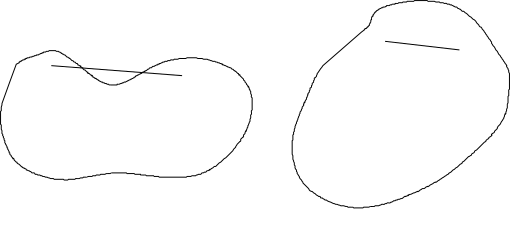
\includegraphics[width=0.8\linewidth]{lect8_6.png}
	
	\; Не выпукло $\quad$ Выпукло
\end{wrapfigure}

\textbf{Упражнение.} Шар в нормированном пространстве --- выпуклое множество. 

\textbf{Пример 2.} $\forall$ выпуклое подмножество нормированного пространства (над $\mathbb{R})$ линейно связно. Доказательство --- см. пример 1. 

\textbf{Пример-упражнение 3.} $X$ --- нормированное пространство над $\mathbb{R}, \; \dim X > 1 \Rightarrow X \backslash \{0\}$ линейно связно. 

\textbf{Пример 4.} $X$ --- нормированное пространство над $\mathbb{R}, \; \dim X > 1.$ Сфера $S = \{x \in X\!\!: ||x|| =  1\}$ линейно связна. 

\begin{wrapfigure}{R}{0.4\textwidth}
		\begin{tikzpicture}
		\draw[->] node[below] {$x$} (0,0) -- (4,2) node[right]{$y$};
		\draw [fill=white] (2,1) circle[radius=.1];
		\draw[->] (0,0) -- (2,0.5) node[below] {$z$};
		\draw[->] (2,0.5) -- (4,2);
		\end{tikzpicture}
		\begin{tikzpicture}
		\coordinate (C) at (3, 2.5);
		\coordinate (O) at (0,0);
		\draw (0,0) circle [radius=2];
		\draw (2.2, -1) node {$S$};
		\draw [fill=black] (0,0) circle [radius=1pt] node[below right] {$O$};
		\draw (O) -- (C);
		\coordinate [label=below:$\frac{x}{||x||}$] (N) at ($(O)!0.4!(C)$);
		\coordinate [label=below right:$x$] (X) at ($(O)!0.8!(C)$);
		\fill [black] (N) circle (1pt);
		\fill [black] (X) circle (1pt);
		\end{tikzpicture}
\end{wrapfigure}

Действительно: рассмотрим $f: \; X \backslash \{0\} \to S, \; f(x) = \dfrac{x}{||x||}.$ 
	
\textbf{Пример 5 ($n$-мерный тор).} Обозначим $S^{1} = \{(x, y) \in \mathbb{R}^{2}: x^{2} + y^{2} = 1\}$ (окружность).

$T^{n} = S^{1} \times ... \times S^{1}$ ($n$ раз) --- $n$-мерный тор. $T^{n}$ линейно связно.

\begin{wrapfigure}{R}{0.3\textwidth}
	\begin{tikzpicture}[x=5cm]
	\draw[domain=0.005:1,samples=5000] plot (\x, {sin((1/\x)r)});
	\end{tikzpicture}
\end{wrapfigure}

\textbf{Упражнение.} Обозначим $X = \{(x, \sin\dfrac{1}{x})\!\!: \; 0 < x \leq 1\} \cup \{(0, y): \; -1 \leq y \leq 1\} \subset \mathbb{R}^{2}.$ 

Доказать: $X$ связно, но не линейно связно. 

\textbf{Определение.} Подмножество $A \subset \mathbb{R}$ --- промежуток $\Leftrightarrow A = (a, b),$ где $-\infty \leq a < b \leq +\infty),$ либо $A = [a, b] \; (-\infty < a \leq b < +\infty),$ либо $A = [a, b),$ где $(-\infty < a < b \leq +\infty),$ либо $A = (a, b] \; (-\infty \leq a < b < +\infty),$ либо $A = \varnothing.$ 

\textbf{Упражнение.} $A$ --- промежуток $\Leftrightarrow A$ выпукло.

\textbf{Предложение.} Следующие свойства подмножества $A \subset \mathbb{R}$ эквивалентны:

(1) $A$ связно, (2) $A$ линейно связно, (3) $A$ --- промежуток. 

\begin{wrapfigure}{R}{0.3\textwidth}
	\begin{tikzpicture}
	\draw[ |-|] node[below, yshift=-0.3] {$a$} (0,0) to  (5,0) node [below] {$b$};
	\draw [black, fill=white] (2,0) circle[radius=1pt] node[below] {$c$};
	\foreach \x in {0, 0.1, ..., 0.4}
	{\draw (\x, 0) -- (\x + 0.1, 0.1) ;}
	\foreach \y in {4.9, 4.8, ..., 4.5}
	{\draw (\y, 0) -- (\y + 0.1, 0.1) ;}
\end{tikzpicture}
\end{wrapfigure}

\textbf{Доказательство.} $(3) \Rightarrow (2)$ --- очевидно, $(2) \Rightarrow (1)$ --- знаем. 

$(1) \Rightarrow (3)\!\!:$ предположим, что $A$ ограничено. Обозначим $a = inf A, \; b = \sup A. \Rightarrow A \subset [a, b].$

Покажем: $(a, b) \subset A.$ (Этого нам достаточно)

Пусть $\exists c \in (a, b),$ т.ч. $c \not \in A.$ Обозначим $U = (-\infty, c) \cap A, \; V = (c, +\infty) \cap A.$

$U, V$ открыты в $A$, $U \cap V = \varnothing,\quad U \cup V = A, \; U \neq \varnothing, \; V \neq \varnothing$ --- противоречие со связностью $A$.

Для неограниченного $A$ рассуждения аналогичны (упражнение). $\square$

\textbf{Следствие (теорема о промежуточном значении)}

$X$ --- связное топологическое пространство, $f \in C(X, \mathbb{R}), \quad x, y \in X \;\; f(x) \leq f(y).$

Тогда $\forall c \in [f(x), f(y)] \; \exists z \in X,$ т.ч. $c = f(z).$

\textbf{Доказательство.} $f(X)$ --- связное подмножество $\mathbb{R} \Rightarrow f(X)$ --- промежуток; $f(x), f(y) \in f(X) \Rightarrow [f(x), f(y)] \subset f(X). \quad \square$

\section{Связные компоненты}

$X$ --- топологическое пространство. 

\textbf{Определение.} \textbf{Связная компонента} --- максимальная (по включению) связное подмножество $X$ (т.е. такое связное подмножество $X,$ которое не содержится ни в каком строго большем связном подмножестве).

\textbf{Синоним:} компонента связности (менее приоритетно).

\subsection{Свойства связных компонентов}

\textbf{Теорема (свойства связных компонентов)}

(1) Связные компоненты образуют разбиение $X$ (т.е.$\forall$ компонент $X_{1}, X_{2} \subset X$ либо $X_{1} = X_{2},$ либо $X_{1} \cap X_{2} = \varnothing,$ и $X$ = объединение всех его связных компонент);

(2) $\forall x \in X$ множество $C(X) = \bigcup \{A \subset X\!: A$ связно, $x \in A\}$ является связной компонентой $X,$ содержащей $x$ (связная компонента точки $x$);

(3) $\forall$ непустое связное $A \subset X$ содержится ровно в одной связной компоненте;

(4) Связные компоненты замкнуты в $X.$

\textbf{Доказательство.} (1), (2): пусть $X_{1}, \; X_{2} \subset X$ --- связные компоненты. Предположим, $X_{1} \cap X_{2} \neq \varnothing.$ Из связности пространств $\Rightarrow X_{1} \cup X_{2}$ связно $\Rightarrow X_{1} = X_{1} \cup X_{2} = X_{2}.$ Из свойств связных пространств: $C(x)$ связно и является наибольшим связных подмножеством, содержащим $x. \Rightarrow C(x)$ --- компонента связности $X \Rightarrow (1), (2).$ 

$(3) \; \exists$ связная компонента $B \subset X,$ т.ч. $A \cap B \neq \varnothing \Rightarrow A \cup B$ связно $\Rightarrow B = A \cup B,$ т.е. $A \subset B.$ Единственность $B$ --- из (1).

$(4)$ Пусть $B \subset X$ --- это связная компонента $\Rightarrow \overline{B}$ связно $\Rightarrow B = \overline{B}$ в силу максимальности $B. \quad \square$ 

\textbf{Следствие.} Если $X$ состоит из конечного числа связных компонент, то эти компоненты не только замкнуты, но еще и открыты в $X.$

\textbf{Доказательство.} $X = C_{1} \cup ... \cup C_{n},$ где $C_{1}, ..., C_{n}$ --- связные компоненты. 

$C_{1} = X \backslash (C_{2} \cup ... \cup C_{n}),$ где $C_{2} \cup ... \cup C_{n}$ замкнуто, $\Rightarrow C_{1}$ открыто. $\square$ 

\textbf{Пример 1.} Связные компоненты $\mathbb{R} \backslash \{0\}$ --- это $(-\infty, 0) \cup (0, +\infty).$ 

\textbf{Пример 2.} $X_{1}, X_{2}$ --- непустые связные топологические пространства, $X = X_{1} \sqcup X_{2} \Rightarrow X_{1}$ и $X_{2}$ ---связные компоненты $X.$

\textbf{Пример 3.} $X$ дискретно $\Leftrightarrow$ связные компоненты $X$ --- одноэлементные множества.

\textbf{Пример 4.} То же самое верно для $X = \mathbb{Q}$ (хотя $\mathbb{Q}$ и не дискретно).

\textbf{Упражнение.} Описать все связные компоненты канторова множества. 

\subsection{Линейно связные компоненты}

\textbf{Определение.} \textbf{Линейно связная компонента} $X$ --- максимальное (по включению) линейно связное подмножество $X.$

\subsection{Свойства линейной связных компонент}

\textbf{Теорема (свойства линейно связных компонент)}

(1) Линейно связные компоненты образуют разбиение $X;$

(2) $\forall x \in X$ множество $PC(x) = \bigcup\{A \subset X\!: A$ линейно связно, $x \in A\}$ является линейно связной компонентой $X,$ содержащей $x$ (линейно связная компонента $x).$ Это множество --- то же самое, что $\{y \in X\!: \exists$ путь из $x$ в $y\};$

(3) $\forall$ непустое линейно связное подмножество $X$ содержится ровно в одной линейно связной компоненте. 

\textbf{Доказательство.} Упражнение (аналогично свойствам связных компонент).

\textbf{Следствие.} Разбиение пространства $X$ на линейно связные компоненты является \textbf{измельчением} разбиения $X$ на связные компоненты, т.е. каждая связная компонента является объединением линейно связных компонент $X),$ --- разбиение на линейно связные компоненты более мелкое, чем на связные.

\textbf{Упражнение.} $X = \{\sin\dfrac{1}{x}\!\!: \quad 0 \leq x \leq 1\} \cup \{(0, \; y)\!\!: \quad -1 \leq y \leq 1\} \subset \mathbb{R}^{2}.$ Описать линейно связные компоненты. Замкнуты ли они?

\subsection{Локально линейно связные пространства}

\textbf{Определение.} Топологическое пространство $X$ \textbf{локально линейно связно} $\Leftrightarrow \; \forall x \in X$ каждая окрестность $x$ содержит линейно связную окрестность $x.$

\textbf{Пример 1.} Открытое подмножество нормированного пространства локально линейно связно.

\textbf{Пример 2.} $\forall$ топологическое многообразие локально линейно связно. 

\textbf{Упражнение.} Произведение топологических многообразий --- топологическое многообразие (в конце доказать по индукции).

\textbf{Предложение.} $X$ --- локально линейно связное топологическое пространство. Тогда его линейно связные компоненты открыты в $X$ и совпадают со связными компонентами. В частности: $X$ связно $\Leftrightarrow$ оно линейно связно.

\textbf{Доказательство.} Пусть $A \subset X$ --- линейно связная компонента. $\forall x \in A \; \exists$ линейно связная окрестность $U_{x} \ni x. \Rightarrow A \cup U_{x}$ линейно связно $\Rightarrow A = A \cup U_{x}$ в силу максимальности $A,$ т.е. $U_{x} \subset A. \Rightarrow A = \underset{x \in A}{\bigcup} U_{x}$ открыто.

Пусть $B$ --- связная компонента $X,$ т.ч. $A \subset B.$ $B \backslash A = \bigcup \{\text{линейно связных компонент X, содержащихся в B и отличных от A}\} \Rightarrow B \backslash A$ открыто $\Rightarrow B = A \cup (B \backslash A),$ где $A, \; B \backslash A$ открыты, $B$ связно $\Rightarrow B \backslash A = \varnothing,$ т.е. $A = B. \quad \square$ 

\section{Компактные топологические пространства}

$X$ --- множество, $\mathfrak{U} \subset 2^{X}.$ 

\textbf{Определение.} $\mathfrak{U}$ --- покрытие подмножества $Y \subset X$ ($\mathfrak{U}$ \textbf{покрывает} $Y$ или $Y$ \textbf{покрывается} семейством $\mathfrak{U}$), если $\bigcup \mathfrak{U} \supset Y.$ Если $X$ --- топологическое пространство, то \textbf{открытое покрытие} $X$ --- это покрытие $X$ открытыми множествами. 

\textbf{Определение.} Топологическое пространство $X$ \textbf{компактно} $\Leftrightarrow$ каждое открытое покрытие $X$ содержит конечное подпокрытие (т.е. конечное подсемейство, покрывающее $X).$

\textbf{Определение.} $X$ --- множество, $\mathfrak{F} \subset 2^{X}.$ $\mathfrak{F}$ --- \textbf{центрированное семейство} $\Leftrightarrow \; \forall$ конечного $\mathfrak{F}_{0} \subset \mathfrak{F} \quad \bigcap \mathfrak{F}_{0} \neq \varnothing.$

\textbf{Предложение.} Топологическое пространство $X$ компактно $\Leftrightarrow$ каждое центрированное семейство его замкнутых поднможеств имеет непустое пересечение. 

\textbf{Доказательство.} Пусть $X - \forall$ множество, $\mathfrak{F} \subset 2^{X}, \; \mathfrak{U} = \{X \backslash F\!: F \in \mathfrak{F}\}.$ Заметим: 

(1) $\bigcap \mathfrak{F} = \varnothing \Leftrightarrow \mathfrak{U}$ --- покрытие $X;$ 

(2) $\mathfrak{F}$ центрированное $\Leftrightarrow$ никакое конечное подсемейство в $\mathfrak{U}$ не покрывает $X.$ 

Из (1), (2) получаем требуемое. $\square$ 

\textbf{Предложение.} $X$ --- топологическое пространство, $Y \subset X.$ $Y$ компактно (в индуцированной топологии) $\Leftrightarrow$ каждое покрытие $Y$ множествами, открытыми в $X,$ имеет конечное подпокрытие. 

\textbf{Доказательство.} $(\Rightarrow)$ Пусть $\{U_{i}\!: i \in I\}$ --- покрытие $Y$ множествами, открытыми в $X.$ Обозначим $V_{i} = U_{i} \cap Y \Rightarrow \{V_{i}\!: i \in I\}$ --- покрытие $Y$ множествами, открытыми в $Y, \Rightarrow \exists i_{1}, ..., i_{n} \in I,$ т.ч. $Y = V_{i_{1}} \cup ... \cup V_{i_{n}} \Rightarrow Y \subset U_{i_{1}} \cup ... \cup U_{i_{n}}.$

$(\Leftarrow)$ Пусть $\{V_{i}\!: i \in I\}$ --- покрытие $Y$ множествами, открытыми в $Y.$ $\forall i \in I \; \exists$ открытое $U_{i} \subset X,$ т.ч. $V_{i} = U_{i} \cap Y. \; \Rightarrow \{U_{i}\!: i \in I\}$ --- покрытие $Y \Rightarrow \exists i_{1}, ..., i_{n},$ т.ч. $Y \subset U_{i_{1}} \cup ... \cup U_{i_{n}} \Rightarrow Y = V_{i_{1}} \cup ... \cup V_{i_{n}} \Rightarrow Y$ компактно. $\square$

\textbf{Пример 1.} Конечное топологическое пространство компактно.

\textbf{Пример 2.} Дискретное пространство компактно $\Leftrightarrow$ оно конечно.

\textbf{Пример 3.} Антидискретное пространство компактно. 

\textbf{Теорема.} Отрезок $[a, b] \subset \mathbb{R}$ компактен. 

\textbf{Доказательство.} См. курс анализа. 

\subsection{Свойства компактных пространств}

\begin{wrapfigure}{R}{0.3\textwidth}
	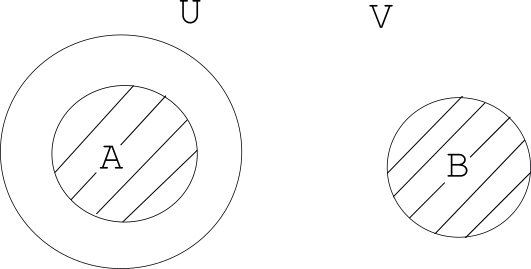
\includegraphics[width = 5cm]{lect9_1.png}
\end{wrapfigure}

\textbf{Теорема (свойства компактных пространств)} 

(1) $f: X \to Y$ непрерывно, $X$ компактно $\Rightarrow f(x)$ компактно;

(2) $X$ компактен, $Y \subset X$ замкнуто $\Rightarrow Y$ компактно;

(3) $X$ --- хаусдорфово, $A, B \subset X$ компактен, $A \cap B = \varnothing \Rightarrow \exists$ открытые $U, V \subset X,$ т.ч. $A \subset U, B \subset V, U \cap V = \varnothing;$

(4) $X$ --- хаусдорфово, $Y \subset X$ компактно $\Rightarrow Y$ замкнуто в $X;$

(5) $X$ --- метрическое пространство, $Y \subset X$ компактно $\Rightarrow Y$ ограничено;

(6) $X$ компактно, $Y$ хаусдорфово, $f: X \to Y$ непрерывно $\Rightarrow f$ замкнуто (т.е. $\forall$ замкнутых $B \subset X \quad f(B)$ замкнуто в $Y$);

(7) $X$ компактно, $Y$ хаусдорфово, $f: X \to Y$ --- непрерывная биекция $\Rightarrow \; f$ --- гомеоморфизм. 

\textbf{Напоминание.} $X$ --- метрическое пространство, $A \subset X.$

$\text{diam} A = \sup\{\rho(x, y)\!: x, y \in A\} \in [0; +\infty]$ --- диаметр $A.$ 

\textbf{Определение.} $A$ ограничено $\Leftrightarrow \text{diam} A < \infty.$ 

\textbf{Предложение.} $A$ ограничено $\Leftrightarrow A$ содержится в некотором шаре. 

\textbf{Доказательство.} $(\Leftarrow) \; A \subset \overline{B}_{r}(x) \Rightarrow \text{diam} A \leq 2r < \infty.$

$(\Rightarrow)$ Обозначается $d = \text{diam} A; \; x \in A \Rightarrow A \subset \overline{B}_{d}(x). \quad \square$ 

\textbf{Доказательство теоремы.} (1) Можем считать: $f(X) = Y.$ Пусть $U \subset 2^{Y}$ --- открытое покрытие $\Rightarrow \{f^{-1}(V)\!: V \in U\}$ --- открытое покрытие $X \; \Rightarrow \exists V_{1}, ..., V_{n} \in U,$ т.ч. $\{f^{-1}(V_{i})\!: 1 \leq i \leq n\}$ --- покрытие $X \overset{f \; \text{сюръекция}}{\Rightarrow} \{V_{i}\!: 1 \leq i \leq n\}$ --- покрытие $Y.$

\begin{wrapfigure}{R}{0.4\textwidth}
	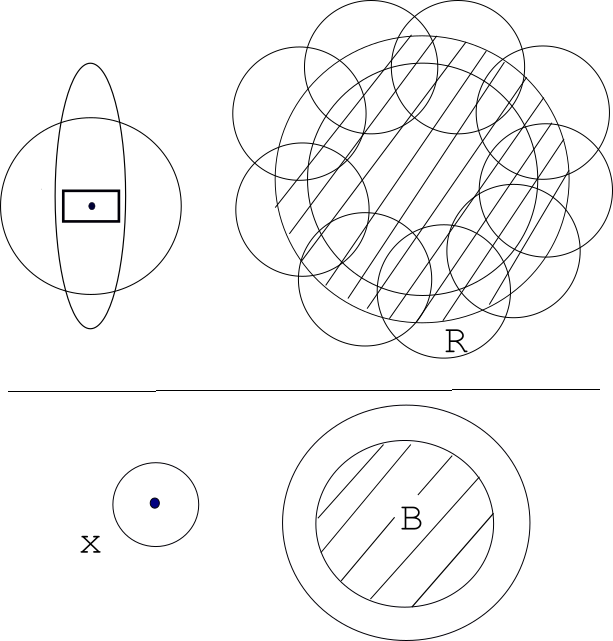
\includegraphics[width = 8cm]{lect9_2.png}
\end{wrapfigure}

(2) Пусть $U$ --- покрытие $Y$ множествами, открытыми в $X \Rightarrow U \cup \{X \backslash Y\}$ --- открытое покрытие $X \Rightarrow \exists V_{1}, ..., V_{n} \in U,$ т.ч. $X = V_{1} \cup .... \cup V_{n} \cup (X \backslash Y) \Rightarrow Y \subset V_{1} \cup ... \cup V_{n} \Rightarrow Y$ компактно. 

(3) Зафиксируем $x \in A. \; \forall y \in B \exists$ открытое $U_{xy} \ni x, V_{xy} \ni y,$ т.ч. $U_{xy} \cap V_{xy} = \varnothing.$

$\{V_{xy}\!: y \in B\}$ --- покрытие $B \Rightarrow B \subset V_{xy_{1}} \cup ... \cup V_{xy_{n}} \overset{\text{обозначим}}{=} V_{x}.$ Обозначим $U_{x} = U_{xy_{1}} \cap ... \cap U_{xy_{n}}.$

$\Rightarrow U_{x}, \; V_{x} \subset X$ открыто, $x \in U_{x}, \; B \subset V_{x}, \; U_{x} \cap V_{x} = \varnothing.$

$\{U_{x}\!: x \in A\}$ --- покрытие $A \Rightarrow A \subset U_{x_{1}} \cup ... \cup U_{x_{n}} \overset{\text{обозначим}}{=} U.$ 

Обозначим $V = V_{x_{1}} \cap ... \cap V_{x_{n}} \Rightarrow U, V \subset X$ --- искомое. 

(4) Пусть $x \in X \backslash Y.$ Применим (4) к $\{x\}$ и $Y \; \Rightarrow \exists$ открытое $U \ni x, \; U \cap Y = \varnothing \Rightarrow x \not \in \overline{Y} \Rightarrow Y = \overline{Y}.$

(5) Зафиксируем $\forall x \in X \Rightarrow X = \underset{r > 0}{\bigcup} B_{r}(x) \Rightarrow \exists r_{1}, ..., r_{n} > 0,$ т.ч. $Y \subset \underset{i = 1}{\overset{n}{\bigcup}} B_{r_{i}}(x) = B_{R}(x),$ где $R = \underset{1 \leq i \leq n}{\max} r_{i}.$ 

(6) Пусть $B \subset X$ замкнуто $\overset{(2)}{\Rightarrow} B$ компактно $\overset{(1)}{\Rightarrow} f(B)$ компактно $\overset{(4)}{\Rightarrow} f(B)$ замкнуто в $Y.$ 

(7) --- частный случай (6) (т.к. гомеоморфизм --- то же, что замкнутая непрерывная биекция). $\quad \square$ 

\textbf{Следствие.} $X$ --- компактное топологическое пространство, $X \neq \varnothing, f \in C(X, \mathbb{R}) \Rightarrow f$ ограничена и принимает наибольшее и наименьшее значения. 

\textbf{Доказательство.} Теорема (1) $\Rightarrow \; f(X) \subset \mathbb{R}$ компактно $\overset{(5)}{\Rightarrow} f(X)$ ограничено, т.е. $f$ ограничена. Обозначим $a = inf f(X), \; b = \sup f(X).$ Из (4) теоремы: $f(X)$ замкнуто в $\mathbb{R} \Rightarrow a, b \in f(X),$ т.е. $a = \underset{x \in X}{\min} f(x), \; b = \underset{x \in X}{\max} f(x). \quad \square$

\section{Некоторые свойства центрированных семейств}

$X$ --- множество. 

\textbf{Определение.} Семейство $\mathfrak{F} \subset 2^{X}$ называется \textbf{центрированным}, если $\forall$ конечного $\mathfrak{F}_{0} \subset \mathfrak{F} \quad \bigcap \mathfrak{F}_{0} \neq \varnothing.$ 

\textbf{Предложение 1.} Топологическое пространство $X$ компактно $\Leftrightarrow \forall$ центрированного семейства $\mathfrak{F}$ замкнутых подмножеств $X$ $\quad \bigcap \mathfrak{F} \neq \varnothing.$ 

\textbf{Доказательство}. Было. 

\textbf{Предложение 2.} Топологическое пространство $X$ компактно $\Leftrightarrow \forall$ центрированного семейства $\mathfrak{F}$ замкнутых подмножеств $X \quad \bigcap \{\overline{A}\!: A \in \mathfrak{F}\} \neq \varnothing.$ 

\textbf{Доказательство.} $(\Leftarrow)$ Из предложения 1. 

$(\Rightarrow)$ Семейство $\{\overline{A}\!: A \in \mathfrak{F}\}$ центрированное. Далее см. предложение 1. $\quad \square$

\textbf{Лемма.} $X, Y$ --- множества. 

(1) $\mathfrak{R} \subset 2^{X}$ --- центрированное семейство, $g: X \to Y$ --- отображение $\Rightarrow \{g(A)\!: A \in \mathfrak{F}\}$ --- центрированное семейство. 

(2) $\forall$ центрированного семейства $\mathfrak{F} \subset 2^{X} \quad \exists$ максимальное центрированное семейство, содержащее $\mathfrak{F},$ т.е. такое центрированное семейство, которое не содержится ни в каком строго большем центрированном семействе подмножеств $X$).

(3) Пусть $\mathfrak{F} \subset 2^{X}$ --- максимальное центрированное семейство $\Rightarrow \forall A_{1}, ..., A_{n} \subset \mathfrak{F}$ выполнено $A_{1} \cap ... \cap A_{n} \in \mathfrak{F}.$ 

\textbf{Доказательство.} (1) $\forall A_{1}, ..., A_{n} \in \mathfrak{F} \quad \underset{i = 1}{\overset{n}{\bigcap}} g(A_{i}) \supset g(\underset{i = 1}{\overset{n}{\bigcap}}A_{i}) \neq \varnothing,$ где $\underset{i = 1}{\overset{n}{\bigcap}} A_{i} \neq \varnothing.$ 

(2) Обозначим $\text{Г} = \{\varepsilon \subset 2^{X}\!: \varepsilon > \mathfrak{F}\}.$

(Г, $\subset$) --- ЧУМ. Покажем: Г удовлетворяет условию леммы Цорна.

Пусть Л $\subset$ Г --- линейно упорядоченное подмножество. Обозначим $\mathfrak{H} = \bigcap \{\varepsilon\!: \varepsilon \in \text{Л}\}.$ Покажем: $\mathfrak{H}$ центрированное. 

Пусть $H_{1}, ..., H_{n} \in \mathfrak{H} \Rightarrow \forall i  = 1, ..., n \quad H_{i} \in \varepsilon_{i},$ где $\varepsilon_{i} \in$ Л. 

$\exists k,$ т.ч. $\varepsilon_{i} \subset \varepsilon_{k} \quad \forall i = 1, ..., n \Rightarrow H_{1}, ..., H_{n} \in \varepsilon_{k} \Rightarrow \overset{n}{\underset{i = 1}{\bigcap}} H_{i} \neq \varnothing \Rightarrow \mathfrak{H}$ центрированное $\Rightarrow \mathfrak{H} \in$ Г и $\mathfrak{H} \supset \varepsilon \quad \forall \varepsilon \in \text{Л} \Rightarrow$ Г удовлетворяет условию Леммы Цорна $\Rightarrow$ в Г есть максимальный элемент. 

(3) Семейство $\{A_{1} \cap ... \cap A_{n}\!: A_{i} \in \mathfrak{F}, \; n \in \mathbb{N}\}$ центрированное и содержит $\mathfrak{F} \Rightarrow$ оно равно $\mathfrak{F}. \quad \square$

\section{Теорема Тихонова (очень важная)}

\textbf{Теорема (А. Н. Тихонов).} $(X_{i})_{i \in I}$ --- семейство компактных топологических пространств $\Rightarrow \underset{i \in I}{\text{П}} X_{i}$ компактно.

\textbf{Доказательство.} Обозначим $X = \underset{i \in I}{\text{П}} X_{i}.$ Пусть $\mathfrak{F} \subset 2^{X}$ --- центрированное семейство. 

Л(2) $\Rightarrow \exists$ максимальное центрированное семейство $\mathfrak{F}_{\max}, \quad \mathfrak{F} \subset \mathfrak{F}_{\max}.$

Достаточно доказать: $\bigcap \{\overline{A}\!: A \in \mathfrak{F}_{\max}\} \neq \varnothing$ (см. предложение 2) $(*)$

$\forall i \in I$ обозначим $p_{i}\!: X \to X_{i}$ каноническую проекцию. 

Семейство $\{p_{i}(A)\!: A \in \mathfrak{F}_{\max}\} \subset 2^{X_{i}}$ --- центрированное (Л(1)). Предложение (2) $\Rightarrow \exists x_{i} \in X_{i},$ т.ч. $x_{i} \in \overline{p_{i}(A)} \quad \forall A \in \mathfrak{F}_{\max}.$ Обозначим $x = (x_{i})_{i \in I} \in X.$ 

Пусть $U$ --- базисная окрестность $x$ вида $U = \underset{i \in J}{\bigcap} p_{i}^{-1}(U_{i}),$ где $J \subset I$ конечноe, $U_{i} \subset X_{i}$ --- открыто. 

Покажем: $U \cap A \neq \varnothing \quad \forall A \in \mathfrak{F}_{\max}.$

$\forall i \in J \quad x_{i} = p_{i}(x) \in U_{i} \Rightarrow U_{i} \cap p_{i}(A) \neq \varnothing \quad A \in \mathfrak{F}_{\max} \Rightarrow p_{i}^{-1}(U_{i}) \cap A \neq \varnothing \quad \forall A \in \mathfrak{F}_{\max}.$

$\overset{\text{Л(3)}}{\Rightarrow} \mathfrak{F}_{\max} \cup \{p_{i}^{-1}(U_{i})\}$ --- центрированное $\Rightarrow p^{-1}(U_{i}) \in \mathfrak{F}_{\max}$ (в силу максимальности) $\forall i \in J.$

$\overset{\text{Л(3)}}{\Rightarrow} U \in \mathfrak{F}_{\max} \Rightarrow \forall A \in \mathfrak{F}_{\max} U \cap A \neq \varnothing \Rightarrow \forall A \in \mathfrak{F}_{\max} \quad x \in \overline{A},$ т.е. $x \in \bigcap \{\overline{A}\!: A \in \mathfrak{F}_{\max} \Rightarrow (*)$ доказано. $\square$ 

\textbf{Следствие.} Подмножество $X \subset \mathbb{R}^{n}$ компактно $\Leftrightarrow$ $X$ замкнуто и ограничено (в евклидовой метрике).

\textbf{Доказательство.} $(\Rightarrow)$ --- из свойств компактных пространств. 

$(\Leftarrow) \; X$ ограничено $\Rightarrow X$ содержится в замкнутом кубе $C \subset \mathbb{R}^{n}, \; C$ компактен как произведение отрезков, $X$ замкнут в $C \Rightarrow X$ компактен. $\square$

\section{Локально компактные пространства}

\textbf{Определение.} Топологическое пространство $X$ \textbf{локально компактно} $\Leftrightarrow \; \forall x \in X \; \exists$ окрестность $U \ni x,$ т.ч. $\overline{U}$ компактно. Предупреждение: в разной литературе локальная компактность может пониматься по-разному.

\textbf{Примеры.} (1) компактность $\Rightarrow$ локальная компактность;

(2) Дискретное пространство локально компактно;

(3) $\mathbb{R}^{n}$ со стандартной топологией локально компактно (хотя само, конечно, не компактно);

(4) (чуть более общий пример) Открытое подмножество в $\mathbb{R}^{n}$ локально компактно; 

\begin{wrapfigure}{R}{0.3\textwidth}
	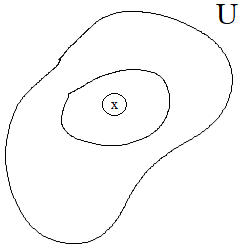
\includegraphics[width = 5cm]{lect10_1.png}
\end{wrapfigure}

(5) Топологическое многообразие локально компактно;

(6) $\mathbb{Q}$ не локально компактно. Действительно: $\forall$ интервала $(a, b)$ замыкание $(a, b) \cap \mathbb{Q}$ в $\mathbb{Q}$ --- это $[a, b] \cap \mathbb{Q}$ --- некомпактно (т.к. в $\mathbb{R}$ он не замкнут);

(7) $\mathbb{R^{N}}$ не локально компактно. Действительно: пусть $U \subset \mathbb{R^{N}}$ --- базисное открытое множество, $U = \underset{i \in \mathbb{N}}{\text{П}} U_{i}, \; U_{i} \subset \mathbb{R},$ причем все $U_{i},$ кроме их конечного числа, --- это $\mathbb{R}.$ Зафиксируем $i \in \mathbb{N},$ т.ч. $U_{i} = \mathbb{R}.$ Обозначим $p_{i}\!: \mathbb{R^{N}} \to \mathbb{R}$ --- каноническая проекция. 

$p_{i}(\overline{U}) = \mathbb{R}$ --- некомпактен $\Rightarrow \overline{U}$ некомпактен $\Rightarrow \mathbb{R^{N}}$ не локально компактен.

\textbf{Предложение (доказательство в других курсах).} Любое бесконечномерное нормированное пространство не локально компактно.

\textbf{Предложение 1.} $X_{1}, ..., X_{n}$ --- локально компактные пространства $\Rightarrow \underset{i = 1}{\overset{n}{\text{П}}} X_{i}$ локально компактно.

\textbf{Доказательство.} $\forall x = (x_{1}, ..., x_{n}) \in \overset{n}{\underset{i = 1}{\text{П}}} x_{i}, \forall i = 1, ..., n \; \exists$ окрестность $U_{i} \ni x_{i},$ т.ч. $\overline{U_{i}}$ компактно. 
	
$U = \overset{n}{\underset{i = 1}{\text{П}}} U_{i}$ --- окрестность $x, \; \overline{U} = \overset{n}{\underset{i = 1}{\text{П}}} \overline{U_{i}}$ (упражнение) $\Rightarrow \overline{U}$ компактно. $\square$
	
\textbf{Наблюдение.} Произведение бесконечного числа локально компактных пространств необязательно локально компактно --- см пример 7.

\textbf{Предложение 2.} $X$ --- локально компактное пространство, $Y \subset X$ замкнуто $\Rightarrow Y$ локально компактно. 

\textbf{Доказательство.} $\forall y \in Y \; \exists U \subset X, \; U \ni y,$ т.ч. $\overline{U}$ компактно.

$U \cap Y$ --- окрестность $y$ в $Y,$ замыкание $U \cap Y$ в $Y$ равно $\overline{U} \cap Y,$ где $\overline{U}, Y$ замкнуты. 

$\overline{U} \cap Y$ --- замкнутое подмножество в $\overline{U} \Rightarrow$ оно компактно. $\square$

\begin{wrapfigure}{R}{0.3\textwidth}
	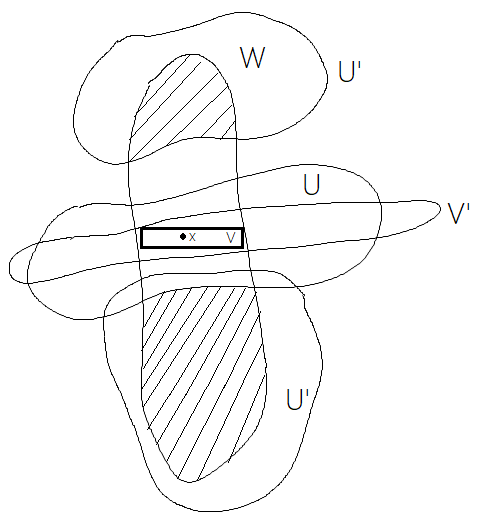
\includegraphics[width = 5cm]{lect10_2.png}
\end{wrapfigure}

\textbf{Предложение 3.} $X$ --- хаусдорфово локальное компактное пространство, $Y \subset X$ открыто $\Rightarrow Y$ локально компактно. 

\textbf{Лемма.} $X$ --- хаусдорфово локальное компактное пространство, $x \in X.$ Тогда $\forall$ окрестности $U \ni x \; \exists$ окрестность $V \ni x,$ т.ч. $\overline{V}$ компактно и $\overline{V} \subset U.$ 

\textbf{Доказательство.} $\exists$ окрестность $W \ni x,$ т.ч. $\overline{W}$ компактно. $K = \overline{W} \backslash U$ замкнуто в $\overline{W} \Rightarrow K$ компактно, $x \not \in K.$

$\exists$ открытые $U', V' \subset X,$ т.ч. $K \subset U', x \in V', U' \cap V' = \varnothing.$ Обозначим $V = V' \cap W.$ $V$ --- окрестность $x; \; \overline{V} \subset \overline{W} \Rightarrow \overline{V}$ компактно. 

$\overline{V} \subset \overline{V'} \cap \overline{W} \subset \overline{(X \backslash U')} \cap \overline{W} = (X \backslash U') \cap \overline{W} \subset (X \backslash K) \cap \overline{W} \subset \overline{W} \backslash K \subset U. \square$

\textbf{Доказательство предложения 3.} $\forall y \in Y \; \exists$ окрестность $V \ni y$ в $X,$ т.ч. $\overline{V}$ компактно, $\overline{V} \subset Y$ (см. лемму) $\Rightarrow V$ --- окрестность $y$ в $Y,$ замыкание $V$ в $Y$ --- это $\overline{V} \cap Y = \overline{V}$ --- компактно. $\quad \square$ 

Пусть $X - \forall$ топологическое пространство.

\section{Одноточечная компактификация}

\textbf{Обозначим} $X_{+} = X \sqcup \{\infty\}$ --- дизъюнктное объединение множеств. 

\textbf{Обозначим} $\tau_{+} = \{U \subset X\!: U$ открыто в $X\} \cup \{U \subset X_{+} \backslash U$ компактно и замкнуто в $X\}.$

\textbf{Упражнение.} $\tau_{+}$ --- топология на $X_{+}.$

\textbf{Определение.} $(X_{+}, \tau_{+})$ --- \textbf{одноточечная компактификация} $X.$

\textbf{Определение.} $X, Y$ --- топологические пространства. Отображение $f\!: X \to Y$ --- \textbf{открытое вложение} $\Leftrightarrow f$ непрерывно, инъективно и открыто. 

\textbf{Наблюдение.} $f$ --- открытое вложение $\Rightarrow f$ --- гомеоморфизм $X$ на $f(X).$

\textbf{Теорема.} $X$ --- топологическое пространство. 

(1) $i_{X}\!: X \to X_{+}$ --- открыто вложение;

(2) $X_{+}$ компактно;

(3) $X_{+}$ хаусдорфово $\Leftrightarrow X$ хаусдорфово и локально компактно;

(4) Если $X$ компактно, то $X_{+}$ --- дизъюнктное объединение $X$ и $\{\infty\}$ как топологических пространств, $\{\infty\}$ --- изолированная точка $X_{+};$

(5) $X$ некомпактно $\Leftrightarrow X$ плотно в $X_{+}.$

\textbf{Доказательство.} (1) $i_{X}$ инъективно (очевидно) и открыто --- из определения $\tau_{+}.$ Докажем непрерывность. $U \subset X_{+}$ открыто. Если $\infty \not \in U \Rightarrow i_{X}^{-1}(U) = U$ и $U$ открыто в $X.$

Если $\infty \in U,$ то $i_{X}^{-1}(U) = U \cap X = X \backslash (X_{+} \backslash U),$ где $(X_{+} \backslash U)$ замкнуто в $X,$ --- открыто в $X.$

(2) Пусть $\{U_{i}\}_{i \in I}$ --- открытое покрытие $X_{+}.$ $\exists j \in I,$ т.ч. $\infty \in U_{j}. \; X_{+} \backslash U_{j}$ компактно, $\{U_{i}\}_{i \in I}$ --- покрытие $X_{+} \backslash U_{j} \Rightarrow \exists i_{1}, ..., i_{n} \in I,$ т.ч. $X_{+} \backslash U_{j} \subset U_{i_{1}} \cup ... \cup U_{i_{n}} \Rightarrow X_{+} = U_{j} \cup U_{i_{1}} \cup ... \cup U_{i_{n}}.$

(3) $(\Rightarrow)$ Пусть $X_{+}$ хаусдорфово. Из (1): топология на $X,$ индуцированная из $X_{+},$ совпадает с исходной топологией на $X \Rightarrow X$ хаусдорфово. 

Пусть $x \in X. \; \exists$ открытые $U, V \subset X_{+},$ т.ч. $x \in U, \infty \in V, U \cap V = \varnothing \Rightarrow U$ --- окрестность $x$ в $X; \; X_{+} \backslash V \Rightarrow \overline{U} \subset X_{+} \backslash V$ (где $\overline{U}$ --- замыкание $U$ в $X) \Rightarrow \overline{U}$ компактно.

$(\Leftarrow)$ Пусть $X$ хаусдорфово и локально компактно, $x, y \in X_{+}, x \neq y.$ Покажем: $\exists$ открытое $U, V \subset X_{+}, U \ni x, V \ni y, U \cap V = \varnothing.$ Если $x, y \in X,$ то такие $U, V \exists,$ т.к. $X$ хаусдорфово.

Пусть $x \in X, y = \infty.$ $\exists$ открытое $U \subset X, \; x \in U,$ т.ч. $\overline{U}$ компактно (где $\overline{U}$ --- замыкание $U$ в $X$). Обозначим $V = X_{+} \backslash \overline{U}.$ $\infty \in V, U \cap V = \varnothing, V$открыто (т.к. $X_{+} \backslash V = \overline{U}$ замкнуто в $X$ и компактно).

(4) $X_{+} \backslash \{\infty\} = X$ --- замыкнуто в $X$ и компактно $\Rightarrow \{\infty\}$ --- открытое подмножество $X_{+} \Rightarrow \{\infty\}$ --- изолированная точка $X_{+}.$ 

$\forall$ открытого $U \subset X_{+} \quad U \cap X$ открыто и $U \cap \{\infty\}$ открыто (как пересечение двух открытых) $\Rightarrow \tau_{+}$ --- топология дизъюнктного объединения $X$ и $\{\infty\}.$

(5) $(\Leftarrow)$ --- из (4). 

$(\Rightarrow)$ Если $X$ не плотно в $X_{+},$ то $\exists$ открытое непустое $U \subset X_{+}, U \cap X = \varnothing \Rightarrow U = \{\infty\} \Rightarrow  X_{+} \backslash U = X$ компактно. $\square$ 

\textbf{Предложение.} $Y$ --- компактное хаусдорфово топологическое пространство, $y_{0} \in Y, X = Y \backslash \{y_{0}\}.$ Определим $f\!: X_{+} \to Y$ так: $f(x) = x \quad \forall x \in X, f(\infty) = y_{0}.$ Тогда $f$ --- гомеоморфизм.

\textbf{Доказательство.} Очевидно, $f$ --- биекция $\Rightarrow$ можем отождествить $X_{+}$ и $Y$ как множества: $y_{0} = \infty.$ Обозначим $\tau =$ исходная топология на $Y.$ Осталось доказать: $\tau = \tau_{+}.$ 

Пусть $U \in \tau.$ Если $y_{0} \not \in U \Rightarrow U$ --- открытое подмножество $X \Rightarrow U \in \tau_{+}.$

Если $y_{0} \in U,$ то $Y \backslash U$ замкнуто в $Y \Rightarrow Y \backslash U$ компактно и содержится в $X.$ Оно замкнуто в $X,$ т.к. $X$ хаусдорфово. 

Доказали, что $\tau \subset \tau_{+}.$ Это значит, что отображение $I\!: (Y, \tau_{+}) \to (Y, \tau), \; I(y) = y,$ непрерывно. Т.к. $(Y, \tau_{+})$ компактно, а $(Y, \tau)$ --- хаусдорфово, то есть $I$ --- непрерывная биекция из компактного пространства в хаусдорфово, то $I$ --- гомеоморфизм $\Rightarrow \tau = \tau_{+}. \quad \square$

\begin{wrapfigure}{R}{0.3\textwidth}
	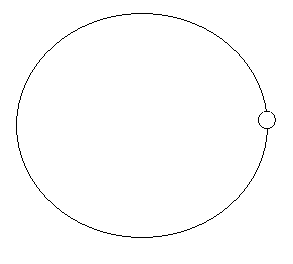
\includegraphics[width = 5cm]{lect10_3.png}
\end{wrapfigure}

\textbf{Примеры.} (1) $[0; 1)_{+} \cong [0; 1]$ (см. предложение).

(2) $(0; 1)_{+} \cong S^{1} \quad S^{1} = \{z \in \mathbb{C}\!: |z| = 1\}.$

$f\!: (0; 1) \to S^{1} \backslash \{1\}, f(t) = e^{2\pi i t}$ --- гомеоморфизм (упражнение). Из предложения $(0, 1)_{+} \cong (S^{1} \backslash \{1\}_{+}) \cong S^{1}.$

(3) (упражнение) $(\mathbb{R}^{2})_{+} \cong S^{2}.$

(4) (упражнение) $(\mathbb{R}^{n})_{+} \cong S^{n}.$

\section{Эквивалентность норм}

$X$ --- векторное пространство над $\mathbb{K} \; (\mathbb{K} = \mathbb{R}, \mathbb{C}).$

Пусть $||\cdot||'$ и $||\cdot||''$ --- нормы на $X; \; \tau', \tau''$ --- порожденные ими топологии на $X.$

\textbf{Определение.} 1) $||\cdot||'$ \textbf{мажорируется} $||\cdot||'' \; (||\cdot||' \prec ||\cdot||'') \Leftrightarrow \tau' \subset \tau'';$

$2) ||\cdot||'$ и $||\cdot||''$ \textbf{эквиваленты} $(||\cdot||' \sim ||\cdot||'') \Leftarrow \tau' = \tau''.$

\textbf{Предложение.} Следующие свойства эквивалентны:

(1) $||\cdot||' \prec ||\cdot||'';$

(2) Из $x_{n} \underset{\tau''}{\to} x \Rightarrow x_{n} \underset{\tau'}{\to} x;$

(3) $\exists C > 0,$ т.ч. $\forall x \in X \; ||x||' \leq C||x||''.$

\textbf{Доказательство.} (1) $\Leftrightarrow$ Отображение $I\!: (X, \tau'') \to (X, \tau'), \; I(x) = x,$ непрерывно $\Leftrightarrow$ оно секвенциально непрерывно $\Leftrightarrow (2).$

$(3) \Rightarrow (2).$ Пусть $x_{n} \underset{\tau''}{\to} x,$ т.е. $||x_{n} - x||'' \to 0 \Rightarrow ||x_{n} - x||' \leq C||x_{n} - x||'' \to 0 \Rightarrow ||x_{n} - x||' \to 0,$ т.е. $x_{n} \underset{\tau'}{\to} x.$

$(2) \Rightarrow (3).$ Пусть (3) не выполнено. $\Rightarrow \forall n \in \mathbb{N} \; \exists x_{n} \in X,$ т.ч. $||x_{n}||' > n^{2}||x_{n}||''.$ Обозначим $y_{n} = \dfrac{x_{n}}{n||x_{n}||''}.$ $||y_{n}||'' = \dfrac{||x_{n}||''}{n||x_{n}||''} = \dfrac{1}{n} \to 0 \Rightarrow y_{n} \underset{\tau''}{\to} 0.$

$||y_{n}||' = \frac{||x_{n}||'}{n||x_{n}||''} > \dfrac{n^{2}||x_{n}||''}{n||x_{n}||''} = n \to \infty \Rightarrow y_{n} \underset{\tau'}{\not \to} 0$ --- противоречие с (2). $\square$

\textbf{Следствие.} $||\cdot||' \sim ||\cdot||'' \Leftrightarrow \exists c, \; C > 0,$ т.ч. $\forall x \in X \quad c||x||' \leq ||x||'' \leq C||x||'.$

\textbf{Теорема.} На конечномерном векторном пространстве любые две нормы эквиваленты. 

\textbf{Доказательство.} Пусть $||\cdot||$ --- какая-либо норма на $\mathbb{K}^{n}.$ Покажем: $||\cdot|| \sim ||\cdot||_{2},$ где $||\cdot||_{2}$ --- евклидова норма: $||x||_{2} = \sqrt{\underset{i = 1}{\overset{n}{\sum}} |x_{i}|^{2}}. \; \forall x = (x_{1}, ..., x_{n} \in \mathbb{K}^{n}).$ 

$||x|| = ||\underset{i = 1}{\overset{n}{\sum}} x_{i}e_{i}|| \leq \underset{i = 1}{\overset{n}{\sum}} |x_{i}||e_{i}|| \leq \sqrt{\underset{i = 1}{\overset{n}{\sum}}|x_{i}|^{2}} \underset{= C}{\sqrt{\underset{i = 1}{\overset{n}{\sum}}||e_{i}||^{2}}} = C||x||_{2} \Rightarrow ||\cdot|| \prec ||\cdot||_{2},$ где $e_{i} = (0...0\underset{(i)}{1}0...0).$

Обозначим $f(x) = ||x||.$ Покажем: $f$ непрерывна на $(\mathbb{K}^{n}, ||\cdot||_{2}).$ $\forall x, y \in \mathbb{K}^{n} \quad |f(x) - f(y)| = |||x|| - ||y||| \leq ||x - y|| \leq C||x - y||_{2} \Rightarrow$ из $x_{n} \underset{||\cdot_{2}||}{\to} x$ следует $f(x_{n}) \to f(x).$

$\Rightarrow f$ секвенциально непрерывна, т.е. непрерывна на $(\mathbb{K}^{n}, ||\cdot||_{2}).$ Обозначим $S = \{x \in \mathbb{K}^{n}\!: ||x||_{2} = 1\}. \; S$ компактна (т.к. замкнута и ограничена). $f$ непрерывна на $S \; \Rightarrow \exists \; \underset{x \in S}{\min} f(x) = a > 0.$
	
$\forall x \in \mathbb{K}^{n} \backslash \{0\}$ рассмотрим $y = \dfrac{x}{||x||_{2}}.$ $y \in S \Rightarrow f(y) = ||y|| \geq a,$ т.е. $||\dfrac{x}{||x||_{2}}|| \geq a,$ т.е. $||x|| \geq a ||x||_{2} \Rightarrow ||\cdot|| \sim ||\cdot||_{2}. \quad \square$

\textbf{Теорема$'$} (эквивалентна предыдущей). Любая норма на $\mathbb{K}^{n}$ задает на $\mathbb{K}^{n}$ топологию произведения $\underbrace{\mathbb{K} \times ... \times \mathbb{K}}_{n}.$

\section{Факторпространства}

Пусть $X$ --- множество, $\sim$ --- отношение эквивалентности на $X.$ 

\textbf{Обозначение.} $\forall x \in X \; [x] = \{y \in X\!: y \sim x\}$ --- \textbf{класс эквивалентности} $x.$

\textbf{Напоминание.} Классы эквивалентности образуют разбиение $X,$ то есть два класса эквивалентности либо равны, либо не пересекаются. 

\textbf{Обозначание.} \textbf{Факторпространство} $X$ по $\sim$ --- это множество $X_{/ \sim} = \{[x]\!: x \in X\}.$

\textbf{Обозначение.} $q\!: X \to X_{/ \sim}, \; q(x) = [x]$ --- \textbf{отображение факторизации.}

Пусть теперь $X$ --- топологическое пространство.

\textbf{Определение.} \textbf{Фактортопология} на $X_{/ \sim}$ --- финальная топология $\tau_{q},$ порожденная $q.$ Т.е.: $U \in \tau_{q} \Leftrightarrow q^{-1}(U)$ открыто в $X.$

\textbf{Определение.} $(X_{/ \sim}, \tau_{q})$ --- \textbf{факторпространство} $X$ по $\sim.$

\textbf{Теорема 1} (свойства фактортопологии)

(1) $\tau_{q}$ --- самая тонкая топология на $X_{/ \sim},$ в которой $q$ непрерывно.

\begin{wrapfigure}{L}{0.25\textwidth}
		\begin{tikzpicture}[node distance=2cm, auto]
	\node (A) {$X$};
	\node(B) [right of=A] {$Y$};
	\node (C) [below of=A] {$X_{/\sim}$};
	\draw[->](A) to node [left]{$q$}(C);
	\draw[->](B) to node [right] {$\quad y$}(C);
	\draw[->](A) to (B);
	\end{tikzpicture}
\end{wrapfigure}

(2) Если $Y$ --- топологическое пространство, то отображение $g\!: X_{/ \sim} \to Y$ непрерывно $\Leftrightarrow g \circ q\!: X \to Y$ непрерывно. 

\textbf{Доказательство.} См. теорему о свойствах финальной топологии. $\square$

\textbf{Теорема 2} (универсальное свойство факторпространств)

\begin{wrapfigure}{L}{0.25\textwidth}
	\begin{tikzpicture}[node distance=2cm, auto]
	\node (A) {$X$};
	\node(B) [right of=A] {$Y$};
	\node (C) [below of=A] {$X_{/\sim}$};
	\draw[->](A) to node [left]{$q$}(C);
	\draw[->](C) to node [right] {$\quad \widetilde{f} \quad \quad (1)$}(B);
	\draw[->](A) to (B);
	\end{tikzpicture}
\end{wrapfigure}

Пусть $Y$ --- топологическое пространство, $f\!: X \to Y$ --- непрерывное отображение, постоянное на классах эквивалентности, т.е. из $x \sim y \Rightarrow f(x) = f(y).$ Тогда $\exists!$ непрерывное $\widetilde{f},$ делающее эту диаграмму коммутативной. 

\textbf{Доказательство.} $\forall u \in X_{/ \sim}$ выберем $\forall x \in u$ и положим $\widetilde{f}(u) = f(x).$ Если $x, y \in u \Rightarrow f(x) = f(y)$ по условию $\Rightarrow \widetilde{f}\!: X_{/\sim} \to Y$ корректно определено. 

По построению $\widetilde{f}$ делает диаграмму (1) коммутативной (т.к. определение $\widetilde{f}$ означает, что $\widetilde{f}(a(x)) = f(x) \; \forall x)$ и является единственным отображением с этим свойством. Из теоремы 1 и непрерывности $f$ получаем непрерывность $\widetilde{f}. \quad \square$

\textbf{Теорема 3.} Пусть выполнены условия теоремы 2. Тогда: 

(1) $\widetilde{f}$ --- сюръекция $\Leftrightarrow f$ --- сюръекция;

(2) $\widetilde{f}$ --- инъекция $\Leftrightarrow \forall x, y \in X$ условия $x \sim y$ и $f(x) = f(y)$ эквивалентны;

(3) Пусть $X$ компактно, $Y$ хаусдорфово и выполнены (1), (2) $\Rightarrow \widetilde{f}$ --- гомеоморфизм.

\textbf{Доказательство.} (1) $\widetilde{f}(X_{/\sim}) = \widetilde{f}(q(X)) = f(X).$

(2) $\widetilde{f}$ --- инъекция $\Leftrightarrow \forall u, v \in X_{/ \sim} (\widetilde{f}(u) = \widetilde{f}(v) \Leftrightarrow u = v) \Leftrightarrow \forall x, y \in X \quad (\underset{= f(x)}{\widetilde{f}(q(x))} = \underset{= f(y)}{\widetilde{f}(q(y))} \Leftrightarrow x \sim y).$

(3) $X$ компактно $\Rightarrow X_{/ \sim} = q(X)$ компактно; из (1), (2): $\widetilde{f}$ --- непрерывная биекция $\Rightarrow \widetilde{f}$ --- гомеоморфизм. $\square$

\textbf{Пример 1.} Введем отношение эквивалентности на $[0, 1]\!: 0 \sim 1,$ остальные классы эквивалентности --- одноэлементные множества. Покажем: \fbox{$[0, 1]_{/\sim} \simeq S^{1}.$}

\begin{figure}[htpb]
	\begin{minipage}{.24\textwidth}
		$S^{1} = \{z \in \mathbb{C}\!: |z| = 1\}$
		\end{minipage}
	\begin{minipage}{.24\textwidth}
		\centering
		\begin{tikzpicture}[node distance=2cm, auto]
		\node (A) {$[0; 1]$};
		\node(B) [below of=A] {$[0; 1]_{/\sim}$};
		\node (C) [right of=A] {$S^{1}$};
		\draw[->](A) to node {$f$}(C);
		\draw[->](B) to node [right] {$\quad \widetilde{f}$}(C);
		\end{tikzpicture}
	\end{minipage}
	\begin{minipage}{.24\textwidth}
		$f(t) = e^{2\pi i t}$
		
		$f$ удовлетворяет условию теоремы 3 $\Rightarrow \widetilde{f}$ --- гомеоморфизм.
	\end{minipage}
	\begin{minipage}{.20\textwidth}
		\quad
		\begin{tikzpicture}[scale=0.6]
		\draw [fill=white] (2,2) circle[radius=2];
		\draw (2,0) -- (2,4);
		\draw (0,2) -- (4,2);
		\draw [fill=black] (4,2) node[right] {$1$} circle[radius=.2];
		\end{tikzpicture}
	\end{minipage}
\end{figure}

\begin{wrapfigure}{L}{0.3\textwidth}
	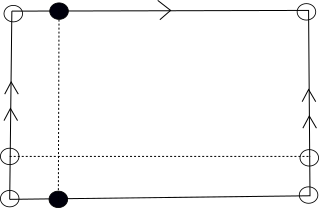
\includegraphics[width = 5cm]{lect11_4.png}
\end{wrapfigure}

\textbf{Пример 2.} Введем отношение эквивалентности на $[0, 1] \times [0, 1]\!:$

$(t, 0) \sim  (t, 1), \; (0, t) \sim (1, t) \; \forall t \in [0, 1].$

Остальные классы эквивалентности --- одноэлементные множества.

Покажем: \fbox{$([0, 1] \times [0, 1])_{/\sim} \simeq T^{2}$}

\begin{wrapfigure}{L}{0.2\textwidth}
	\begin{tikzpicture}[node distance=2cm, auto]
	\node (A) {$[0; 1]^{2}$};
	\node(B) [below of=A] {$[0; 1]^{2}_{/\sim}$};
	\node (C) [right of=A] {$T^{2}$};
	\draw[->](A) to node {$f$}(C);
	\draw[->](A) to (B);
	\draw[->](B) to node [right] {$\quad \widetilde{f}$}(C);
	\end{tikzpicture}
\end{wrapfigure}

$f(s, t) = (e^{2\pi s}, e^{2\pi i t}). \; f$ удовлетворяет условию теоремы 3 $\Rightarrow \widetilde{f}$ --- гомеоморфизм.

\textbf{Пример 3.} Введем отношение эквивалентности на $\mathbb{R}\!: x \sim y \Leftrightarrow x - y \in \mathbb{Q}.$ Покажем: топология на $\mathbb{R}_{/\sim}$ антидискретна. 

Пусть $U \subset \mathbb{R}_{/\sim}$ открыто, непусто $\Rightarrow q^{-1}(U) \subset \mathbb{R}$ открыто, непусто и инвариантно относительно сдвигов на различные числа (т.е. если $x \in q^{-1}(U),$ то $\forall r \in \mathbb{Q} \; x + r \in q^{-1}(U)) \Rightarrow q^{-1}(U) = \mathbb{R} \Rightarrow U = q(q^{-1}(U)) = q(\mathbb{R}) = \mathbb{R}_{/\sim} \Rightarrow$ фактортопология антидискретна. 

\section{Частный случай фактопространств: стягивание подмножества в точку}

X --- топологическое пространство, $A \subset X.$

Введем на X отношение эквивалентности: $x \sim y \Leftrightarrow$ либо $x = y,$ либо $x, y \in A.$

\textbf{Обозначение.} X / A = X / $\sim$. 

Говорят, X / A получено из X \textbf{стягиванием A в точку.}

\begin{wrapfigure}{L}{0.2\textwidth}
	\begin{tikzpicture}[node distance=2cm, auto]
	\node (Y) {$Y$};
	\node(X1) [right of=Y] {$X_{+}$};
	\node (X) [below of =Y] {$X$};
	\draw[->](X) to node [left]{$\text{вкл}$}(Y);
	\draw[->](Y) to node {$f$}(X1);
	\draw[->](X) to node [right]{$\quad \text{вкл}$}(X1);
	\end{tikzpicture}
\end{wrapfigure}

\textbf{Пример 1.} $[0, 1] / \{0, 1\} \cong S^{1}$ (см. прошлую лекцию).

\textbf{Лемма.} Пусть $Y$ --- хаусдорфово топологическое пространство, $X \subset Y$ --- открытое множество. Рассмотрим f: $Y \to X_{+}, \; f(x) = \begin{cases} x, \text{если} \; x \in X, \\ \infty, \text{если} \; x \not \in X. \end{cases}$

\textbf{Доказательство.} Пусть $U \subset X_{+}$ открыто. Предположим: $\infty \not \in U \Rightarrow U \subset X, U$ открыто в $X \Rightarrow f^{-1}(U) = U \Rightarrow U$ открыто в $Y.$

Пусть теперь $\infty \in U \Rightarrow K = X_{{+}_{\backslash U}} \subset X, \; K$ компактен $\Rightarrow K$ замкнут в $Y \Rightarrow f^{-1}(U) = Y \; f^{-1}(K) = Y \; K$ --- открыто в $Y. \; \square$ (Доказали, что прообраз открытого открыт $\Rightarrow$ доказательство окончено.)

\begin{wrapfigure}{L}{0.4\textwidth}
	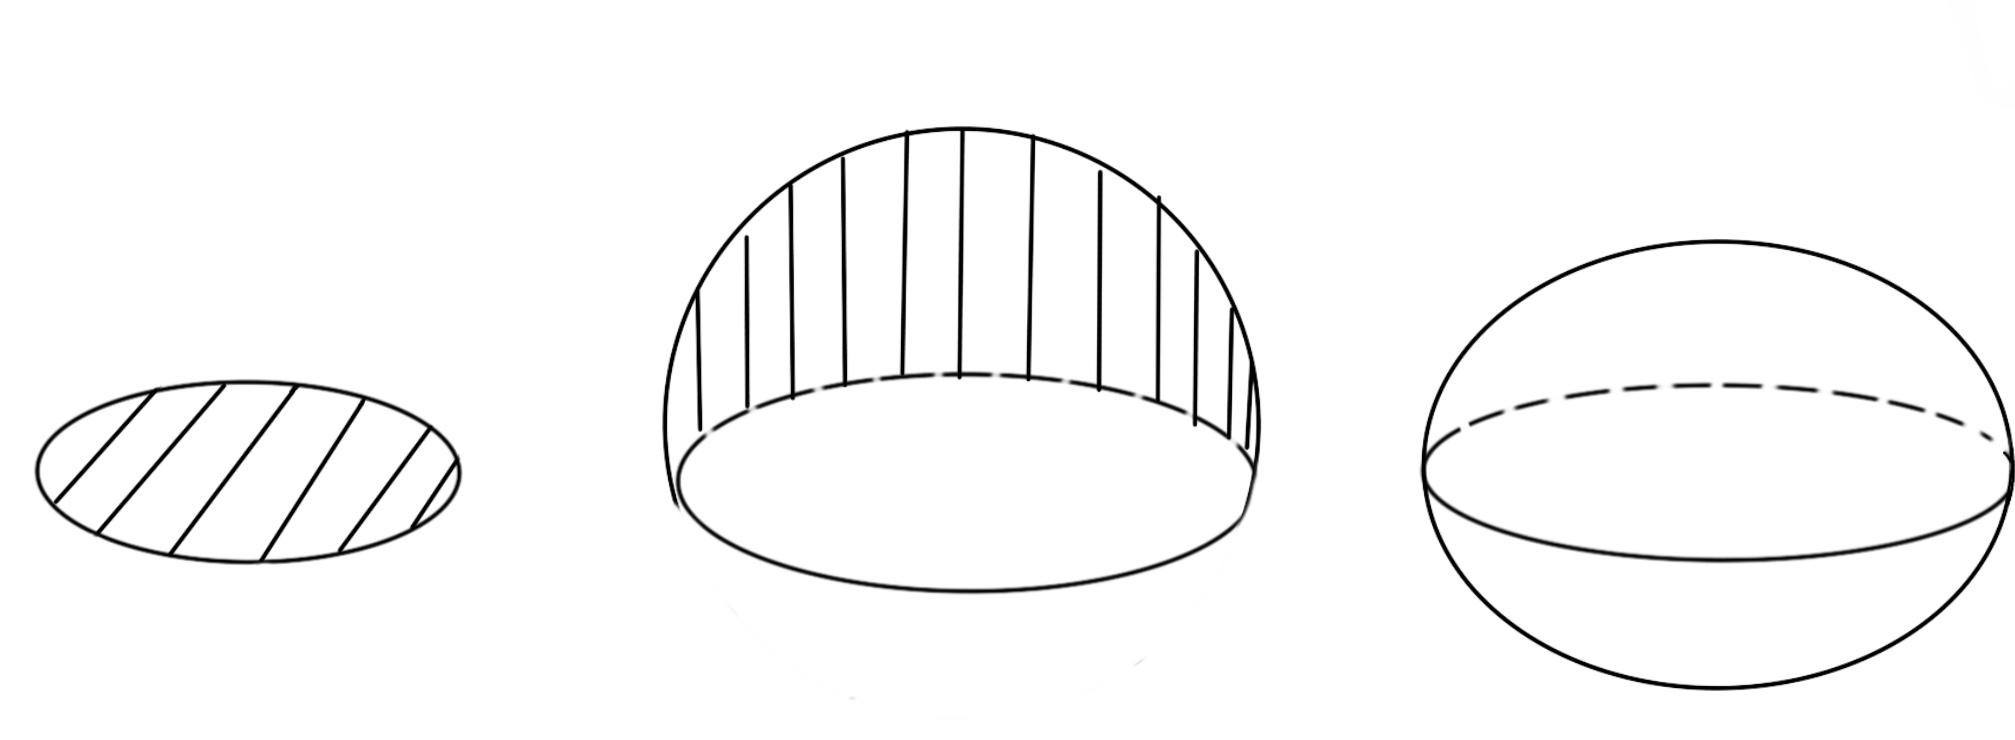
\includegraphics[width = 7 cm]{lect12_2.png}
	\\ \;\\
		\begin{tikzpicture}[node distance=2cm, auto]
		\node (D0) {$\overline{D}$};
		\node(D1) [right of=D0] {$D_{+}$};
		\node (S) [right of=D1] {$S^{2}$};
		\node (D) [below of=D1] {$D$};
		\draw[-](D0) to node {$f$}(D1);
		\draw[-](D1) to node {$\varphi$}(S);
		\draw[->](D) to node [right]{$\text{вкл}$}(S);
		\draw[->](D) to node {$\text{вкл}$}(D0);
		\end{tikzpicture}
\end{wrapfigure}

\textbf{Пример 2.} $D = \{(x, y) \in \mathbb{R}^{2}\!: x^{2} + y^{2} < 1\}.$

$\overline{D} = \{(x, y)\!: \in \mathbb{R}^{2}\!: x^{2} + y^{2} \leq 1\}, S^{1} = \partial \overline{D}.$ Покажем: \fbox{$\overline{D} / S^{1} \cong S^{2}.$} 

Знаем: $D_{+} \cong \mathbb{R}^{2}_{+} \cong S^{2}.$

Зафиксируем гомоморфизм $\varphi\!: D_{+} \to S^{2}.$

$f(x) = \begin{cases} x, \; \text{если} \; x \in D, \\ \infty, \text{если} \; x \in S^{1}. \end{cases}$ Из леммы: f непрерывна.

Обозначим $g = \varphi \circ f\!: \overline{D}/S^{1} \cong S^{2}.$

\subsection{Частный случай факторпространств: склейка по отображению}

$X, \; Y$ --- топологические пространства, $A \subset Y, f\!: A \to X$ непрерывно.

Введем отношение эквивалентности на $X \sqcup Y\!: a \sim f(a) \; \forall a \in A,$ остальные классы эквивалентности --- одноэлементные множества.

\textbf{Обозначение.} $X \cup_{f} Y = (X \sqcup Y) / \sim$ --- склейка $X$ и $Y$ по $f.$

\begin{wrapfigure}{L}{0.2\textwidth}
	\begin{tikzpicture}[node distance=2cm, auto]
	\node (X) {$X$};
	\node(Y) [right of=X] {$Y$};
	\node (X1) [below of=X] {$X_{/\sim}$};
	\draw[->](X) to node [left]{$q$}(X1);
	\draw[->](X1) to node [right]{$\quad \widetilde{f}$}(Y);
	\draw[->](X) to node {$f$}(Y);
	\end{tikzpicture}
\end{wrapfigure}

$X$ --- топологическое пространство, $\sim$ --- отношение эквивалентности.

$\forall x \in X \; [x] = \{y \in X\!: y \sim x.$

$X_{/ \sim} = \{[x]\!: x \in X$ \quad $q\! X \to X_{/\sim}$ \quad q(x) = [x].

$U \subset X_{/\sim}$ открыто $\underset{\text{определение}}{\Leftrightarrow} q^{-1}(U)$ открыто в $X.$

\textbf{Теорема 2} (универсальное свойство факторпространств)

f непрерывна, $x \sim y \Rightarrow f(x) = f(y).$ Тогда $\exists!$ непрерывна $\widetilde{f},$ т.ч. диаграмма коммутативна.

\textbf{Теорема 3.} Пусть выполняются условия теоремы 2. Тогда

(1) $\widetilde{f}$ --- сюръекция $\Leftrightarrow$ f --- сюръекция;

(2) $\widetilde{f}$ --- инъекция $\Leftrightarrow \forall x, y \in X (x \sim y \Leftrightarrow f(x) = f(y)).$

\begin{wrapfigure}{L}{0.4\textwidth}
	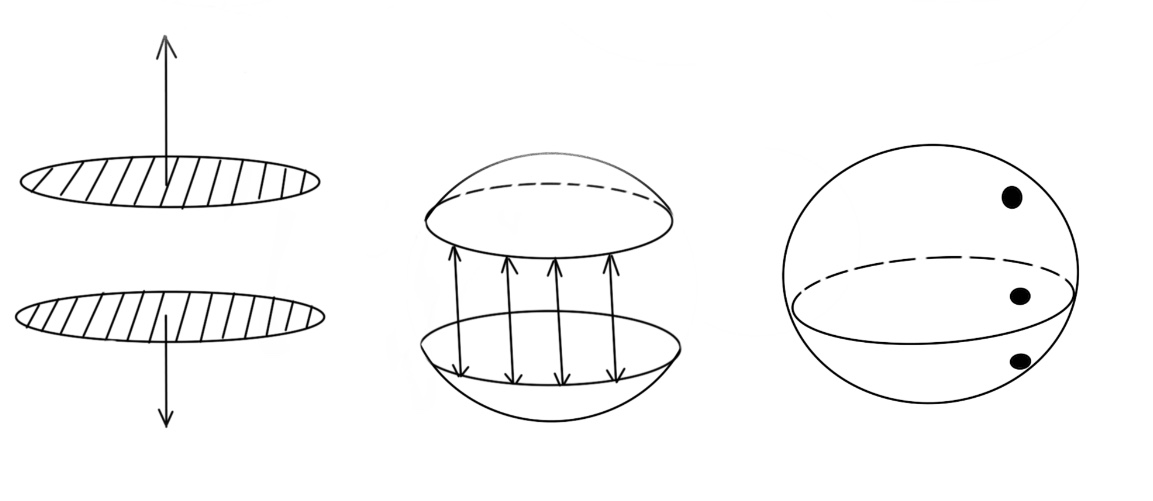
\includegraphics[width = 7 cm]{lect12_5.png}
\end{wrapfigure}

(3) Если (1), (2) выполнены, X компактно, Y хаусдорфово, то $\widetilde{f}$ --- гомеоморфизм.

\textbf{Пример 3.} Рассмотрим $f = i_{s^{1}}\!: S^{1} \to \overline{D}$ --- отображение включения.

Покажем: \fbox{$\overline{D} \cup_{f} \overline{D} \cong S^{2}.$}

Обозначим: $\overline{D_{1}} = \{(p, 1)\!: p \in \overline{D}\}.$

$\overline{D_{-1}} = \{(p, -1)\!: p \in \overline{D}\}.$

$\overline{D} \cup D = \overline{D_{1}} \sqcup \overline{D_{1}}.$

Рассмотрим $g\!: \overline{D_{1}} \sqcup \overline{D_{-1}} \to S^{2}, \; g(x, y, \sqrt{1 - x^{2} - y^{2}}, \; g(x, y, -1) = (x, y, -\sqrt{1 - x^{2} - y^{2}},$ где $(x, y) \in \overline{D}.$

$g$ непрерывно (свойства дизъюнктных объединений).

$g$ сюръективно.

Пусть $p, q \in \overline{D_{1}} \sqcup \overline{D_{-1}}, p \neq q.$

Если $q(p) = g(p),$ то либо $p \in \overline{D_{1}}, \; q \in \overline{D_{-1}},$ либо наоборот.

Пусть $p \in \overline{D_{1}}, \; q \in \overline{D_{-1}}.$

Тогда $g(p) = g(q) \Leftrightarrow g(p) = g(q) = (x, y, 0), x^{2} + y^{2} = 1 \Leftrightarrow 1) p \in \partial \overline{D_{1}} = S^{1}, \; q = f(p), 2) p \sim q.$

$\Rightarrow g$ удовлетворяет условию Теоремы 3 $\Rightarrow \overline{D_{1}} \cup_{f} \overline{D_{-1}} \cong S^{2}.$

\hrulefill

Пусть $X, Y$ --- топологические пространства, $f\!: X \to Y.$

\textbf{Определение.} $f$ --- \textbf{факторное} $\Leftrightarrow f$ сюръективно, топология на $Y$ совпадает с финальной топологией, порожденной $f \Leftrightarrow [f$ сюръективно, $U \subset Y$ открыто $\Leftrightarrow f^{-1}(U)$ открыто в X.]

\textbf{Наблюдение.} (1) Факторное $\Rightarrow$ непрерывное.

(2) Сюръективное $f\!: X \to Y$ --- факторное $\Leftrightarrow [B \subset Y$ замкнуто $\Leftrightarrow f^{-1}(B)$ замкнуто в X.]

\begin{wrapfigure}{L}{0.2\textwidth}
		\begin{tikzpicture}[node distance=2cm, auto]
		\node (X) {$X$};
		\node(Y) [right of=X] {$Y$};
		\node (X1) [below of=X] {$X_{/\sim}$};
		\draw[->](X) to node [left]{$q$}(X1);
		\draw[->](X1) to node [right]{$\quad \widetilde{f}$}(Y);
		\draw[->](X) to node {$f$}(Y);
		\end{tikzpicture}
\end{wrapfigure}

\textbf{Теорема 4.} Пусть $X, Y$ --- топологические пространства, $\sim$ --- отношение эквивалентности на $X, \; q\!: X \to X / \sim$ --- отображение факторизации, $f\!: X \to Y$ непрерывно.

Предположим, $[f(x) = f(y) \Leftrightarrow x \sim y].$

Тогда: $[\widetilde{f}$ --- гомеоморфизм $\Leftrightarrow f$ --- факторное].

\textbf{Доказательство.} $(\Rightarrow)$ Пусть $\widetilde{f}$ --- гомеоморфизм $\Rightarrow \widetilde{f}$ --- сюръекция $\Rightarrow f$ сюръекция (Теорема 3).

Пусть $U \subset Y, \; f^{-1}(U)$ открыто.

$U$ открыто $\Leftrightarrow \; \widetilde{f}^{-1}(U)$ открыто $\Leftrightarrow \underset{= f^{-1}(U)}{q^{-1}(\widetilde{f}^{-1}(U))}$ открыто. Поэтому f факторное.

$(\Leftarrow)$ Пусть f факторное. $\widetilde{f}$ --- непрерывная биекция (из Теоремы 2 и Теоремы 3).

Пусть $U \subset X / \sim$ открыто.

Из коммутативности диаграммы и из биекции $\widetilde{f} \quad f^{-1}(\widetilde{f}(U)) = q^{-1}(U)$ --- открыто в X, f факторное $\Rightarrow \widetilde{f}(U)$ открыто $\Rightarrow \widetilde{f}$ --- гомеоморфизм. $\square$

Пусть $X, Y$ --- множества, $f\!: X \to Y$ --- сюръекция.

\textbf{Определение.} \textbf{Насыщение} множества $A \subset X$ (относительно f) --- это множество $f^{-1}(f(A)).$ A \textbf{насыщено}, если $f^{-1}(f(A)) = A.$

\textbf{Наблюдение.} Введем отношение эквивалентности на $X\!: \; x \sim y \Leftrightarrow f(x) = f(y).$

(1) $\forall A \subset X \quad f^{-1}(f(A)) = \bigcup \{[a]\!: a \in A\}.$

(2) $A$ насыщенно $\forall a \in A \; [a] \subset A \Leftrightarrow A$ --- объединение некоторого семейства классов эквивалентности $\Leftrightarrow A = f^{-1}(B)$ для некоторого $B \subset Y$ (в этом случае $B = f(A)$).

\textbf{Теорема 5.} $X, Y$ --- топологические пространства, $f\!: X \to Y$ --- непрерывная сюръекция.

Следующие утверждения эквивалентны:

(1) f --- факторное;

(2) $\forall$ насыщенного открытого $U \subset X \quad f(U)$ открыто в $Y;$

(3) $\forall$ насыщенного замыкания $B \subset X \quad f(B)$ замкнут в $Y.$

\textbf{Доказательство.} $(1) \Rightarrow (2)$ Пусть f факторное, $U \subset X$ открыто и насыщенно.

$f^{-1}(f(U)) = U$ --- открыто $\Rightarrow f(U)$ открыто.

$(2) \Rightarrow (1)$ Пусть $V \subset Y$ таково, что $f^{-1}(V)$ открыто в $X.$

$f^{-1}(V)$ насыщенно и открыто $\Rightarrow f(f^{-1}(V))$ открыто, но $f(f^{-1}(V)) = V \Rightarrow$ открыто $\Rightarrow (1).$

\textbf{Следствие 1.} $X, Y$ --- топологические пространства, $f\!: X \to Y$ --- непрерывная сюръекция, $f$ открыто либо замкнуто $\Rightarrow f$ факторное.

\textbf{Следствие 2.} X, Y --- топологические пространства, $f\!: X \to Y$ --- факторное, $Z \subset X$ --- открыто либо замкнуто, Z насыщенно $\Rightarrow f_{\backslash Z}\!: Z \to f(Z)$ --- факторное.

\textbf{Следствие 3.} X, Y --- топологические пространства, $f\! X \to Y$ --- непрерывная сюръекция, X компактно, Y хаусдорфово $\Rightarrow f$ --- факторное.

\textbf{Примечание} X, Y --- топологические пространства, $X \neq \varnothing, Y \neq \varnothing.$

Введем отношение эквивалентности на $X \times Y\!: (x_{1}, y_{1}) \sim (x_{2}, y_{2}) \Leftrightarrow x_{1} = x_{2}.$

Рассмотрим $\rho\!: X \times Y \to X, \; \rho(x, y) = x. \quad \rho$ открыто (упражнение) и сюръективно $\Rightarrow$ $\rho$ факторное.

$\quad \quad \rho(u) = \rho(v) \Leftrightarrow u \sim v. \quad$ Из Теоремы 4: $(X \times Y)_{/\sim} \cong X.$

\textbf{Предложение.} X --- топологическое пространство, $\sim$ --- отношение эквивалетности, $q\!: X \to X_{/\sim}$ --- отображение факторизации. Тогда $X_{/\sim}$ хаусдорфово $\Leftrightarrow \forall x, y \in X,$ т.ч. $x \sim y, \; \exists$ открытое насыщение множеств $U, V \subset X,$ т.ч. $[x] \subset U, y \subset V, \; U \cap V = \varnothing.$

\textbf{Доказательство.} Заметим: $\exists$ биекция между множествами $\{W \subset X_{/\sim}\!: W$ открыто\} и $\{U \subset X\!: U$ открыто и насыщенно\}: $w \mapsto q^{-1}(w), \; U \mapsto q(U). \quad \square$

\textbf{Пример. Вещественное проективное пространство.} $n \in \mathbb{N}, \; \mathbb{R}{P}^{n} = \{l \subset \mathbb{R}^{n + 1}\!:$ l --- векторное подпространство, $\dim l = 1\}.$

$\mathbb{R}\mathbb{P}^{n}$ снабжается финальной топологией, порожденной отображением $f\!: \mathbb{R}^{n + 1}\backslash\{0\} \to \mathbb{R}\mathbb{P}^{n}, \; f(v) = \text{span}{v} = \{\lambda v\!: \lambda \in \mathbb{R}\}.$

Эквивалентно: $\mathbb{R}{P}^{n} = (\mathbb{R}^{n + 1}\backslash\{0\})/\sim,$ где $u \sim v \Leftrightarrow u = \lambda v, \; \lambda \in \mathbb{R}\backslash\{0\}.$

\textbf{Обозначение.} $S^{n} = \{x \in \mathbb{R}^{n + 1}\!: ||x||_{2} = 1\}.$

\textbf{Предположение.} $\mathbb{RP}^{n} \cong S^{n}/\sim,$ где $x \sim y \Leftrightarrow x = \pm y.$

\textbf{Доказательство.}

\begin{figure}[htpb]
	\centering
	\begin{minipage}{.40\textwidth}
		\begin{tikzpicture}[node distance=2cm, auto]
		\node (A) {$S^{n}$};
		\node(B) [below of=A] {$S^{n}_{/\sim}$};
		\node (D) [right of=A] {$\mathbb{R}^{n + 1}\backslash\{0\}$};
		\node (E) [right of=D] {$S^{n}$};
		\node (C) [below of=D] {$\mathbb{RP}^{n}$};
		\node (F) [below of=E] {$S^{n}_{/\sim}$};
		\node (G) [below of=A] {$S^{n}_{/\sim}$};
		\draw[->](A) to node {$i$}(D);
		\draw[->](D) to node {$p$}(E);
		\draw[->](A) to node [left]{$q_{1}$}(G);
		\draw[->](G) to node {$f$}(C);
		\draw[->](C) to node {$g$}(F);
		\draw[->](D) to node {$q_{2}$}(C);
		\draw[->](E) to node {$q_{1}$}(F);
		\end{tikzpicture}
	\end{minipage}
	\begin{minipage}{.40\textwidth}
		$\bullet \; i$ --- отображение включения;
		
		$\bullet \; q_{1}, \; q_{2}$ --- отображение факторизации.
	\end{minipage}
\end{figure}

$q_{2}i$ постоянно на классах эквивалентности $\Rightarrow \exists ! f,$ т.ч. диаграмма коммутативна, f непрерывна (свойства факторпространств). Заметим: f --- биекция (см. Теорему 3 из позапрошлой лекции). $p\!: \mathbb{R}^{n + 1} \backslash \{0\} \to S^{n}, \; p(v) = \dfrac{v}{||v||_{2}}.$

$q_{1}p$ постоянно на классах эквивалентности $\Rightarrow \exists! g,$ т.ч. диаграмма коммутативна, g непрерывна.

$p_{i} = \text{id}_{S^{n}} \Rightarrow gf = \text{id}S^{n}/_{\sim}$ (см. утверждение о единственности в универсальном свойстве факторпространств) $\Rightarrow g = f^{-1} \Rightarrow f^{-1}$ непрерывна $\Rightarrow f$ --- гомеоморфизм. $\square$

\textbf{Предложение.} $\mathbb{RP}^{n}$ --- компактно и хаусдорфово. 

\textbf{Доказательство.} $\mathbb{RP}^{n} \cong S^{n}_{\sim}, \; S^{n}$ --- компактна $\Rightarrow S^{n}_{/\sim} = q(S^{n})$ компактна (q непрерывно). 

Пусть $x, y \in S^{n}, s \not\sim y \Rightarrow x, y, -x, -y$ попарно различны $\Rightarrow \exists r > 0,$ т.ч. $Br(x), Br(y), Br(-x), Br(-y)$ попарно не пересекаются. 

$U = (Br(x) \cup Br(-x)) \cap S^{n}.$

$V = (Br(y) \cup Br(-y)) \cap S^{n}.$

Тогда $U, \; V$ открыто в $S^{n}, \; U \cap V = \varnothing, \; U \ni [x], \; V \ni [y]$ насыщенны $\Rightarrow S^{n}_{/\sim}$ хаусдорфово. $\square$

\section{Нормальные пространства. Лемма Урысона}

\subsection{Нормальные пространства}

\textbf{Определение.} Топологическое пространство X --- \textbf{$T_{1}$-пространство} $\Leftrightarrow \forall x \in X \; \{x\}$ замкнут в $X.$

\textbf{Наблюдение.} Хаусдорфово $\Rightarrow T_{1}$-пространство.

\textbf{Определение.} $X$ --- топологическое пространство. 

(1) X называется \textbf{регулярным} $\Leftrightarrow X - T_{1}-$пространство, $\forall x \in X, \; \forall$ замкнутого $B \subset X,$ т.ч. $x \notin B \; \exists$ открытые $U, V \subset X, \; x \in U, \; B \subset V, U \cap V = \varnothing. \quad (*)$

(2) X называется \textbf{нормальным} $\Leftrightarrow X - T_{1}-$пространство, $\forall$ замкнутых $A, B \subset X\!: A \cap B = \varnothing \quad \exists$ открытые $U, V \subset X\!: A \subset U, B \subset V, \; U \cap V = \varnothing. \quad (*)$

\textbf{Наблюдение.} Нормальное $\Rightarrow$ регулярное $\Rightarrow$ хаусдорфово.

\textbf{Предложение.} X --- $T_{1}-$пространство.

(1) X регулярно $\Leftrightarrow \forall x \in X, \; \forall$ открытого $W \ni x, \; \exists$ открытая $U,$ т.ч. $x \in U \subset \overline{U} \subset W.$

(2) X нормально $\Leftrightarrow \forall$ замкнутого $A \subset X, \; \forall$ открытого $W \supset A \; \exists$ открытая $U,$ т.ч. $A \subset U \subset \overline{U} W.$

\textbf{Доказательство.} (2) X нормально $\Leftrightarrow \forall$ замкнутого $A \subset X, \forall$ открытого $W \subset X \; (W = X \backslash B,$ где B из определения), т.ч. $A \subset U, C \subset W, U \subset C \Leftrightarrow \forall$ замкнутого $A \subset X, \forall$ открытого $W \supset A \; \exists$ открытое $U,$ т.ч. $A \subset U \subset \overline{U} \subset W.$

(1) Аналогично. $\square$

\textbf{Предложение.} X --- локально компактное хаусдорфово топологическое пространство $\Rightarrow$ X регулярное.

\textbf{Доказательство.} Ранее доказывали $(*)$ для локально компактных хаусдорфовых пространств.

\textbf{Предложение.} (1) $\forall$ компактное хаусдорфово топологическое пространство нормально.

(2) $\forall$ метризуемое пространство нормально.

\textbf{Определение.} $(X, \rho)$ --- метризуемое пространство, $A \subset X, x \in X.$

$\rho(x, A) = \int\{\rho(x, a)\!: a \in A\}$ --- расстояние от x до A.

\textbf{Лемма.} X --- метризуемое пространство, $A \subset X.$

(1) $\rho(x, A) = 0 \Leftrightarrow x \in \overline{A}.$

(2) Функция $f(x) = \rho(x, A).$ Тогда $|f(x) - f(y)| \leq \rho(x, y).$ Как следствие --- f непрерывна. 

\textbf{Доказательство.} (1) --- упражнение.

(2) $\forall x, y \in X, \forall a \in A \quad \rho(x, a) \leq \rho(x, y) + \rho(y, a).$ x, y фиксированные. Берем $\underset{a \in A}{\inf} \Rightarrow f(x) \leq \rho(x, y) + f(y) \Rightarrow f(x) - f(y) \leq \rho(x, y).$

$\underset{\leftarrow}{\overset{\rightarrow}{x  y}}$ $\Rightarrow f(y) - f(x) \leq \rho(x, y) \Rightarrow |f(y) - f(x)| \leq \rho(x, y).$

Если $x_{n} \to x \Rightarrow |f(x_{n}) - f(x)| \leq \rho(x_{n}, x) \to 0 \Rightarrow f(x_{n}) \to f(x) \Rightarrow f(x) \Rightarrow f$ непрерывна. $\square$

\textbf{Доказательство предложения.} (1) X --- компактное хаусдорфово топологическое пространство, $A, B \subset X$ замкнуто, $A \cap B = \varnothing \Rightarrow A, B$ компактно. Из свойств компактных пространств мы заключаем, что $\exists$ открытые $U, V \subset X,$ т.ч. $A \subset U. \; B \subset V, \; U \cap V = \varnothing.$

(2) $(X, \rho)$ --- метрическое пространство, $A, B \subset X$ замкнуто, $A \cap B = \varnothing.$

Рассмотрим функцию $\varphi(x) = \dfrac{\rho(x, A)}{\rho(x, B) + \rho(x, A)}, \; \varphi\!: X \to [0; 1].$

Лемма $\Rightarrow \varphi$ непрерывна, $\varphi_{/A} = 0, \; \varphi_{/B} = 1.$

Предположим, $U = \varphi^{-1}([0, \dfrac{1}{2}]), \; V = \varphi^{-1}([\dfrac{1}{2}, 1]).$

$U, V$ открыты, $U \cap V = \varnothing, A \subset U, B \subset V \Rightarrow X$ нормально. $\quad \square$

\subsection{Лемма Урысона}

\textbf{Лемма Урысона.} X --- нормальное топологическое пространство, $A, B \subset X$ замкнуты, $A \cap B = \varnothing.$ Тогда $\exists$ непрерывная $f\!\!: X \to [0; 1],$ т.ч. $f|_{A} = 0, f|_{B} = 1.$ 

\begin{wrapfigure}{R}{0.4\textwidth}
	\begin{tikzpicture}[scale=0.5]
	\draw [fill=white] (0,0) circle[radius=200pt] node[right] {$U_{1}$};
	\draw [fill=white] (0,0) circle[radius=120pt] node[right] {$U_{3/4}$};
	\draw [fill=white] (0,0) circle[radius=60pt];
	\draw [fill=white] (0,0) circle[radius=30pt];
	\draw [fill=white] (0,0) circle[radius=15pt] node{$A$};
	\node[below] at (2,2) {$U_{1/2}$};
	\node[below] at (1.5,1) {$U_{1/4}$};
	\node[below] at (3,3) {$U_{3/4}$};
	\node[below] at (4,4) {$U_{1}$};
	\node[below] at (5.5,6) {$B$};
	\draw (6, 4) -- (7, 5);
	\draw (6.5, 3) -- (7.5, 4);
	\draw (7, 2) -- (8, 3);
	\draw (7.3, 1) -- (8.3, 2);
	\end{tikzpicture}
\end{wrapfigure}

\textbf{Доказательство.} Обозначим $U_{1} = X \backslash B \quad U_{1}$ открыто, $A \subset U_{1} \Rightarrow \exists$ открытое $U_{1/2},$ т.ч. $A \subset U_{1/2} \subset \overline{U}_{1/2} \subset U_{1}.$

$\exists$ открытое $U_{1/4}, U_{3/4},$ т.ч. $A \subset U_{1/4} \subset \overline{U}_{1/4} \subset U_{1/2} \subset \overline{U}_{1/2} \subset U_{3/4} \subset U_{3/4} \subset \overline{U}_{3/4} \subset U_{1}.$ 

И так далее.

Обозначим $D = \{r \in (0; 1]\!: r$ --- двоично-рационально\} = \{$\frac{k}{2^{n}}\!: n \in \mathbb{N}, k = 1, ..., 2^{n}$\}.

D плотно на [0, 1] --- упражнение.

По индукции: $\exists$ семейство открытых множеств $\{U_{t}\!: t \in D\},$ т.ч. $\forall r, s \in D, r < s,$ выполнено $A \subset U_{r} \subset \overline{U}_{r} \subset U_{s} \subset \overline{U_{s}} \subset U_{1}.$

Рассмотрим $f\!: X \to [0; 1], f(x) = \begin{cases} 1, \; \text{если} \; x \in B, \\ \inf\{r \in D\!: x \in U_{r}\}, \text{если} \; x \notin B. \end{cases}$

Тогда $f|_{B} = 1, f|_{A} = 0.$

Докажем: f непрерывна. Достаточно доказать: $\forall t \in (0; 1)$ множества $f^{-1}([0, t))$ и $f^{-1}((t, 1])$ открыты. (Т.к. полуинтервалы [0, b), (a, 1] образуют предбазу топологии на [0, 1]).

\begin{wrapfigure}{L}{0.2\textwidth}
	\begin{tikzpicture}
	\draw[-](0,0) -- (2.6, 0);
	\draw[thick] (0.5,-.1) node[below]{f(x)} -- (0.5,0.1);
	\draw[thick] (2,-.1) node[below]{t} -- (2,0.1);
	\end{tikzpicture}
\end{wrapfigure}

$x \in f^{-1}([0, t)) \Leftrightarrow f(x) < t \Leftrightarrow \exists r \in D,$ т.ч. $x \in U_{r}, r < t \Leftrightarrow x \in \underset{\underset{r < t}{r \in D}}{\bigcup}{U_{r}}.$ Следовательно, $f^{-1}([0, t)) = \underset{\underset{r \in D}{r < t}}{\bigcup} U_{r}$ --- открыто.

$x \in f^{-1}((t, 1]) \Leftrightarrow f(x) > t \Leftrightarrow \exists s \in D,$ т.ч. s > t и $x \notin U_{s} \Leftrightarrow \exists r \in D,$ т.ч. r > t и $x \notin \overline{U_{r}},$ т.е. $x \in X \backslash \overline{U}_{r}.$

\begin{wrapfigure}{L}{0.3\textwidth}
	\begin{tikzpicture}
	\draw (0,0) -- (5,0);
	\draw[thick] (1,0) node[below] {$t$};
	\draw[thick] (2,0) node[below] {$s$};
	\draw[thick] (3,0) node[below] {$f(x)$};
	\foreach \y in {5.0, 4.9, ..., 3}
	{\draw (\y, 0) -- (\y + 0.1, 0.1) ;}
	\end{tikzpicture}
\end{wrapfigure}

Следовательно, $f^{-1}((t, 1]) = \underset{\underset{r \in D}{r > t}}{\bigcup} (X \backslash \overline{U}_{r})$ --- открыто $\Rightarrow f$ непрерывна. $\square$

\textbf{Теорема (Титце, Урысон) (дополнительная, доказательство в следующих курсах).} X --- нормальное топологическое пространство, $Y \subset X$ --- замкнутое подмножество. Тогда $\forall g \in C(Y, \mathbb{R}) \quad \exists f \in C(X, \mathbb{R}),$ т.ч. $f|_{Y} = g.$ Если при этом $g(Y) \in [a, b],$ то и $f$ можно выбрать так, что $f(X) \subset [a, b].$ 
\end{document}